%************************************************
\chapter{The Cosmic Mass Standard Model}\label{ch:standard-model}
%************************************************

\chapterlead{One fixed angle gives every body one triangle; all the triangles of one size make one ellipse; the ellipses make one frame; and in that frame every body of ordinary matter, from the electron to the nucleus of oganesson, has its own place.}

\scene{Belfast, August 1874}

In August 1874 the British Association for the Advancement of Science held its yearly meeting in Belfast, and on one of its mornings George Johnstone Stoney read a short paper to the section of mathematics and physics. Stoney was forty-eight. As a young man he had worked at Birr Castle beside the great telescope of the Earl of Rosse; since 1857 he had been the secretary of the Queen's University of Ireland, an administrative post that left physics to his spare time.

His starting point was Faraday's law of electrolysis. When a current splits water or salt, the amount of matter set free is fixed by the amount of electricity that passes. Stoney read the law the other way round. \enquote{For each chemical bond which is ruptured within an electrolyte,} he wrote, \enquote{a certain quantity of electricity traverses the electrolyte which is the same in all cases} \citep{Stoney1894}. Electricity, then, comes in equal portions, and nature itself supplies the size of one portion. From the number of molecules in a gas, known only roughly at the time, he estimated it at \enquote{a twentieth (that is $10^{-20}$) of the quantity of electricity which was at that time called the ampere}, about sixteen times too small, as Robert Millikan's oil drops would show forty years later \citep{Millikan1913}.

Stoney did something bolder with his portion of electricity. He put it beside two other constants that nature supplies, the speed of light and the constant of gravitation, and built from the three of them a whole system of units of length, time and mass \enquote{in which there shall be nothing arbitrary} \citep{Stoney1894}. His paper waited seven years for print \citep{Stoney1881}. In 1891 he gave his portion of electricity a name, the \emph{electron}, and six years later J.~J. Thomson found the particle that carries it \citep{Thomson1897}.

Written with today's value of the charge, Stoney's unit of mass is $e\sqrt{K/G} \approx 1.85921 \times 10^{-9}$ kg, a little less than two micrograms. Chapter~\ref{ch:interaction} met this number without naming it, as the charge part of the electron and as the charge part of the proton (\Cref{fig:two-parts}). This chapter gives it its name and puts it to work. It is the step of the charge side of every particle triangle, in the same way that the dalton is the step of the mass side, and with it the triangles of all ordinary matter can be drawn in one frame.

\bigskip

Chapter~\ref{ch:interaction} ended with the law read in its own plane: Newton's gravity and Coulomb's law, each at full strength, in the relative plane whose Composer axis leans at $79.86^\circ$, the angle at which like charges push apart (\Cref{subsec:which-root}). This chapter starts from that fixed angle, builds a geometric frame from it one step at a time, and then places in that frame the 306 bodies of ordinary matter for which mass and charge are known: the electron, the proton and the neutron, the 118 atoms of the periodic table, 67 common ions, and the 118 bare nuclei.

\begin{remark}[The Angle Held Fixed]\label{rem:sm-fixed-angle}
In this chapter the angle of the Composer axis is held fixed at $\pb \approx 79.86^\circ$, with $\sin\pb \approx 0.98438$, $\cos\pb \approx 0.17605$ and $2\cos\pb \approx 0.35210$ (\Cref{tab:two-roots}).
\end{remark}

We call the result the \emph{Cosmic Mass Standard Model}. The name borrows a phrase that physics already uses for its theory of elementary particles and forces, so it is worth saying at once what is meant here. The model of this chapter is a standard frame: one set of coordinates, the same for every body, in which each body of ordinary matter has a fixed place, much as each element has its fixed place in the periodic table. It does not replace the Standard Model of particle physics and makes no claim about new particles. It shows the bodies we know, all at once, in the geometry of the cosmic mass.

\paragraph{The road through this chapter.}
The chapter climbs in six steps, shown in \Cref{fig:sm-map}, and each step takes one tool of Chapter~\ref{ch:general-numbers}. \Cref{sec:sm-triangle} draws one body as one triangle, the triangle of a General Number (\Cref{thm:triangle}, Remark~\ref{rem:corner}), and names the Stoney mass. \Cref{sec:sm-ellipse} draws all the triangles of one size at once and finds that they fill an ellipse (\Cref{thm:ellipse}). \Cref{sec:sm-frame} stacks the ellipses of all sizes into a polar-like frame, the rings and rays of Definition~\ref{def:rings-rays}. \Cref{sec:sm-where} shows where real matter falls in that frame, close to the axes (Proposition~\ref{prop:near-axis}), and why two lenses are needed to see it. \Cref{sec:sm-cards} computes the identity cards of all 306 bodies, and \Cref{sec:sm-model} plots them together: the Cosmic Mass Standard Model.

\begin{figure}[tb]
\myfloatalign
\begin{tikzpicture}[>=Stealth,
    mapstep/.style={draw=RoyalBlue!55, fill=RoyalBlue!6, rounded corners=2pt, text width=2.3cm,
                 align=flush center, inner sep=3.5pt, font=\footnotesize, minimum height=2.45cm, anchor=north},
    mapflow/.style={->, thick, RoyalBlue!70}]
  \node[mapstep] (s1) at (1.475,0) {\textbf{1. One body,\\ one triangle}\\[1pt]
    {\color{gray!75!black}\Cref{sec:sm-triangle}}\\[4pt]
    angles $\alpha, \phi, \pb$;\\ the Stoney mass};
  \node[mapstep] (s2) at (4.425,0) {\textbf{2. All triangles:\\ one ellipse}\\[1pt]
    {\color{gray!75!black}\Cref{sec:sm-ellipse}}\\[4pt]
    one ellipse\\ for each size $r$};
  \node[mapstep] (s3) at (7.375,0) {\textbf{3. One frame}\\[1pt]
    {\color{gray!75!black}\Cref{sec:sm-frame}}\\[4pt]
    rings of equal $r$,\\ rays of equal $\alpha$};
  \node[mapstep] (s4) at (1.475,-3.05) {\textbf{4. Where matter falls}\\[1pt]
    {\color{gray!75!black}\Cref{sec:sm-where}}\\[4pt]
    the lean $\delta$;\\ two lenses};
  \node[mapstep] (s5) at (4.425,-3.05) {\textbf{5. Identity cards}\\[1pt]
    {\color{gray!75!black}\Cref{sec:sm-cards}}\\[4pt]
    atoms, ions,\\ nuclei, e, p, n};
  \node[mapstep] (s6) at (7.375,-3.05) {\textbf{6. The standard model}\\[1pt]
    {\color{gray!75!black}\Cref{sec:sm-model}}\\[4pt]
    306 bodies\\ in one frame};
  \draw[mapflow] (s1.east) -- (s2.west);
  \draw[mapflow] (s2.east) -- (s3.west);
  \draw[mapflow, rounded corners=4pt] (s3.south) -- ++(0,-0.3) -| ($(s4.north)+(0,0.3)$) -- (s4.north);
  \draw[mapflow] (s4.east) -- (s5.west);
  \draw[mapflow] (s5.east) -- (s6.west);
  \node[font=\footnotesize, text=gray!75!black, align=center] (c1) at (1.475,1.05) {from Chapter~\ref{ch:general-numbers}:\\ the triangle};
  \node[font=\footnotesize, text=gray!75!black, align=center] (c2) at (4.425,1.05) {from Chapter~\ref{ch:general-numbers}:\\ the ellipse};
  \node[font=\footnotesize, text=gray!75!black, align=center] (c3) at (7.375,1.05) {from Chapter~\ref{ch:general-numbers}:\\ rings and rays};
  \draw[->, gray!70] (c1.south) -- (s1.north);
  \draw[->, gray!70] (c2.south) -- (s2.north);
  \draw[->, gray!70] (c3.south) -- (s3.north);
  \node[font=\footnotesize, text=gray!75!black, align=center, anchor=east] (c4) at ($(s4.west)+(-0.3,-1.22)$) {from\\ Chapter~\ref{ch:general-numbers}:\\ close to the\\ Composer axis};
  \draw[->, gray!70] (c4.east) -- ++(0.3,0);
\end{tikzpicture}
\caption[The road through the chapter]{The road through the chapter, from one fixed angle to one frame for all ordinary matter. Each box is one step, with the section where it is taken, and each step stands on a tool of Chapter~\ref{ch:general-numbers}.}
\label{fig:sm-map}
\end{figure}

%------------------------------------------------
\section{Step 1: One Body, One Triangle}\label{sec:sm-triangle}
%------------------------------------------------

Remarks~\ref{rem:identity} and~\ref{rem:identity-triangle} give every body a new identity card, the triplet $(r, \alpha, \phi)$, and draw it as a triangle (\Cref{fig:sm-triangle}). Its three sides are the mass $m$, laid along the mass axis from the origin $O$ to the corner $P$; the charge part $q\Gp$, laid from $P$ to the tip $Q$ along the direction of the Composer axis; and the cosmic magnitude $r$, the base $OQ$. Its three angles are:
\begin{itemize}
  \item the \emph{charge phase angle} $\alpha$ at $O$, which faces the charge side $q\Gp$;
  \item the \emph{mass phase angle} $\phi$ at $Q$, which faces the mass side $m$;
  \item the angle at the corner $P$, where the two sides meet. Because the charge side always leaves the mass axis at the angle $\pb$, this corner is always $180^\circ - \pb \approx 100.14^\circ$ when $m$ and $q\Gp$ have the same sign, and $\pb \approx 79.86^\circ$ when their signs differ (Remark~\ref{rem:corner}).
\end{itemize}
The three angles of a triangle add up to $180^\circ$, so $\alpha + \phi = \pb$ (Remark~\ref{rem:identity}). This is the whole of the geometry. From one body to the next only the two sides change; the corner angle never does.

\begin{figure}[tb]
\myfloatalign
\begin{tikzpicture}[x=1mm, y=1mm, >=Stealth, every node/.style={font=\small}]
  % (m, q G) = (2, 1.5): r = 2.7030, alpha = 33.111 deg, phi = 46.749 deg
  \coordinate (O) at (0,0); \coordinate (P) at (40,0); \coordinate (Q) at (45.282,29.531); \coordinate (X) at (70,0);
  \draw[->, gray] (-4,0) -- (74,0) node[right] {mass axis};
  \draw[gray, dashed] ($(P)!-0.18!(Q)$) -- ($(P)!1.32!(Q)$) node[above] {Composer axis};
  \draw[very thick, Maroon!85!black] (O) -- (P) node[midway, below] {mass $m$};
  \draw[very thick, RoyalBlue] (P) -- (Q) node[pos=0.55, right=2pt, align=left, font=\footnotesize] {charge part\\ $q\Gp = z\,m_S$};
  \draw[very thick] (O) -- (Q) node[pos=0.55, above left=-1pt, font=\footnotesize] {cosmic magnitude $r$};
  \pic [draw, "$\alpha$", angle radius=10mm, angle eccentricity=1.3] {angle = P--O--Q};
  \pic [draw, "$\phi$", angle radius=7mm, angle eccentricity=1.4] {angle = O--Q--P};
  \pic [draw, angle radius=4.2mm] {angle = Q--P--O};
  \node[font=\footnotesize] at ($(P)+(150:8.2)$) {$100.14^\circ$};
  \pic [draw, gray, "$\pb$", angle radius=7mm, angle eccentricity=1.35] {angle = X--P--Q};
  \fill (O) circle (1.3pt); \fill (P) circle (1.1pt); \fill (Q) circle (1.5pt);
  \node[anchor=north east] at (-0.5,-0.5) {$O$}; \node[anchor=north] at ($(P)+(0,-4.3)$) {$P$}; \node[anchor=south east] at ($(Q)+(-0.6,0.4)$) {$Q$};
\end{tikzpicture}

\caption[One body, one triangle]{One body, one triangle, drawn to scale at $79.86^\circ$. The mass $m$ runs along the mass axis from $O$ to $P$, the charge part $q\Gp = z\,m_S$ runs from $P$ to $Q$ along the direction of the Composer axis, and the cosmic magnitude $r$ closes the triangle. The corner at $P$ is always $100.14^\circ$ when the two parts have the same sign. The drawing uses $m = 2$ and $q\Gp = 1.5$ in any unit of mass, which give $r \approx 2.703$, $\alpha \approx 33.11^\circ$ and $\phi \approx 46.75^\circ$.}
\label{fig:sm-triangle}
\end{figure}

\subsection{The Stoney Mass}\label{subsec:sm-stoney}

The mass side of a triangle can take any value, but the charge side cannot. Every free body in nature carries a whole number of elementary charges, $q = z\,e$, where $z$ is the charge number: $z = -1$ for the electron, $z = +1$ for the proton, $z = +3$ for the iron ion Fe$^{3+}$, and $z = Z$, the atomic number, for a bare nucleus. (Quarks carry thirds of $e$, but no quark has ever been seen on its own.) The charge side $q\Gp = z\,e\,\Gp$ is therefore always a whole number of steps of one fixed length.

\begin{definition}[Stoney Mass]\label{def:stoney-mass}
The \textbf{Stoney mass} is the charge part of one elementary charge, the size of $e\,\Gp$ with $\Gp = \sqrt{K/G}$ (\Cref{subsec:relative-plane}):
\begin{align*}
m_S := e\sqrt{\frac{K}{G}} &\approx 1.602177 \times 10^{-19}\ \mathrm{C} \times 1.16043 \times 10^{10}\ \mathrm{kg/C} \\
&\approx 1.85921 \times 10^{-9}\ \mathrm{kg}.
\end{align*}
A body of charge number $z$ has the charge part $q\Gp = z\,m_S$, laid along the Composer axis.
\end{definition}

\begin{remark}[The Stoney Mass and the Planck Mass]\label{rem:stoney-planck}
The Stoney mass has two meanings.
\begin{enumerate}
  \item \emph{Balance.} The Composer Unit was sized so that $\Gp^2 G = K$ (\Cref{subsec:relative-plane}). Multiplied by $e^2$, this reads $G\,m_S^2 = K e^2$: two bodies of mass $m_S$, each carrying one elementary charge, attract each other by gravity exactly as strongly as they repel each other electrically. They are a balanced pair: in the laws of Newton and Coulomb, two such bodies can rest at any distance from each other. More generally, two bodies of positive mass are a balanced pair exactly when their charge phase angles add up to $\pb$, or to $\pb + 180^\circ$ when both charges are negative (\Cref{prop:law-cards}); a body of mass $m_S$ with one elementary charge has two equal parts and lies on the ray $\alpha = \pb/2 \approx 39.93^\circ$.
  \item \emph{The Planck mass.} With the reduced Planck constant $\hbar$ and the speed of light $c$, the Planck mass is $m_P = \sqrt{\hbar c/G} \approx 2.17643 \times 10^{-8}$ kg, and the fine-structure constant is $\alpha_{\mathrm{fs}} = K e^2/(\hbar c) \approx 1/137.036$. Then
  \begin{align*}
  m_S^2 &= \frac{K e^2}{G} = \frac{K e^2}{\hbar c}\cdot\frac{\hbar c}{G} \\
  &= \alpha_{\mathrm{fs}}\, m_P^2, \\
  m_S &= \sqrt{\alpha_{\mathrm{fs}}}\; m_P \approx 0.0854245\, m_P .
  \end{align*}
  One Planck mass is $1/\sqrt{\alpha_{\mathrm{fs}}} \approx 11.706$ Stoney masses.
\end{enumerate}
\end{remark}

The fine-structure constant is written $\alpha_{\mathrm{fs}}$ here, so that it is not confused with the charge phase angle $\alpha$.

\scene{Berlin, May 1899}

Twenty-five years after Stoney's paper, Max Planck was working on a problem that had nothing to do with electricity: how much light, of each color, a hot body gives off. In May 1899 he presented to the Prussian Academy of Sciences a paper on the radiation of heat in which a new constant of nature appeared; he wrote it $b$, and we now write it $h$. At the end of the paper he noticed what Stoney had noticed before him. With his new constant, the speed of light, the constant of gravitation and a constant of heat, it was possible to set up units of length, mass, time and temperature which, \enquote{independent of special bodies or substances, necessarily retain their meaning for all times and for all civilizations, even extraterrestrial and non-human ones} \citep{Planck1899}.

Planck did not use the electric charge, and Stoney had not used Planck's constant, which did not yet exist. Their two units of mass therefore differ, and the number that links them was named only later. In 1916 Arnold Sommerfeld, explaining the fine splitting of the lines of hydrogen, met a pure number made of $e$, $\hbar$ and $c$, about $1/137$ \citep{Sommerfeld1916}. That number, the fine-structure constant, is exactly the bridge of Remark~\ref{rem:stoney-planck}: the Stoney mass is the Planck mass times its square root. Planck's own unit of mass, written with $h$ instead of $\hbar$, was $\sqrt{hc/G} \approx 5.46 \times 10^{-8}$ kg; today's Planck mass, $2.17643 \times 10^{-8}$ kg, is about $22$ micrograms, roughly the mass of a small grain of sand.

In the frame of this chapter the Planck mass will appear as one ring among others, at $11.706$ Stoney masses, between the nuclei of sodium ($Z = 11$) and magnesium ($Z = 12$). Every nucleus from magnesium on has a cosmic magnitude larger than the Planck mass. This is a fact about sizes in the frame, not a new physical threshold: nothing happens to a nucleus at the Planck ring.

\begin{workedexample}[Worked example: the identity card of Fe$^{3+}$]
The iron ion Fe$^{3+}$ is an iron atom that has lost three electrons. Its charge number is $z = 3$.
\begin{itemize}
  \item \emph{Mass.} The atomic mass of iron is $55.845$ u. Three electrons, each $0.000548580$ u, are taken away: $m = 55.845 - 3 \times 0.000548580 \approx 55.843354$ u, or, with $1\ \mathrm{u} = 1.66053907 \times 10^{-27}$ kg, $m \approx 9.27301 \times 10^{-26}$ kg.
  \item \emph{Charge part.} By \Cref{def:stoney-mass}, $q\Gp = 3\,m_S \approx 5.57763 \times 10^{-9}$ kg, about sixty million billion times the mass.
  \item \emph{Magnitude.} Remark~\ref{rem:identity-triangle} at $79.86^\circ$ gives $r^2 = m^2 + (q\Gp)^2 + 0.35210\,m\,q\Gp$. The mass changes $r$ by less than one part in $10^{17}$, so $r \approx 5.57763 \times 10^{-9}$ kg $= 3\,m_S$.
  \item \emph{Angles.} The tiny mass tips the triangle away from the charge axis by an angle $\delta$, which Remark~\ref{rem:lean} below gives as $\delta \approx 5.0374 \times 10^{-17}{}^\circ \times 55.843354/3 \approx 9.3768 \times 10^{-16}$ degree. So $\alpha = 79.86^\circ - 9.3768 \times 10^{-16}{}^\circ$ and $\phi = 9.3768 \times 10^{-16}$ degree, and indeed $\alpha + \phi = 79.86^\circ$.
\end{itemize}
\end{workedexample}

\begin{plainwords}
Charge comes in whole numbers of $e$, so the charge side of every triangle is a whole number of Stoney masses: one for the electron and the proton, three for Fe$^{3+}$, ninety-two for the nucleus of uranium. The Stoney mass is to the charge side what the dalton is to the mass side, the step of the ladder. It is also the mass of a speck whose gravity exactly balances the electric push of one elementary charge, and it is a fixed fraction, about one twelfth, of the Planck mass.
\end{plainwords}

%------------------------------------------------
\section{Step 2: All Triangles at Once: The Cosmic Mass Ellipse}\label{sec:sm-ellipse}
%------------------------------------------------

One angle is fixed and two sides are free. What shape holds all the triangles that this angle allows? To find out, we keep the size of the triangle fixed and let its shape change.

\subsection{Eight Frames of a Film}\label{subsec:sm-film}

Fix the base of the triangle, the cosmic magnitude $r$, and take it as the unit of length, $r = 1$. Its two base angles are $\alpha$ and $\phi$, and they always add up to $\pb \approx 79.86^\circ$. Now let $\alpha$ grow, step by step, from $0$ to $79.86^\circ$, so that $\phi$ shrinks from $79.86^\circ$ to $0$. \Cref{fig:sm-film} shows eight frames of this film. By Remark~\ref{rem:mass-charge-rep}, each frame has the two sides
\[
m = \frac{\sin\phi}{\sin\pb} = \frac{\sin(79.86^\circ - \alpha)}{0.98438}, \qquad q\Gp = \frac{\sin\alpha}{\sin\pb} = \frac{\sin\alpha}{0.98438}.
\]
At the start of the film the charge side is almost nothing and the triangle lies nearly flat on its base: a nearly neutral body. At the end the mass side is almost nothing: a nearly pure charge. In between, the two sides trade length, and in frame~4, near $\alpha = \phi = 39.93^\circ$, they are equal.

\begin{figure}[tb]
\myfloatalign
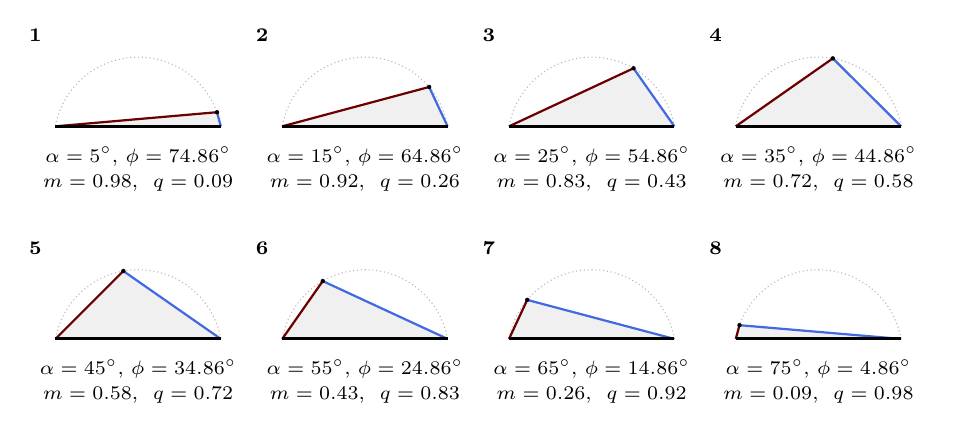
\begin{tikzpicture}[x=1mm, y=1mm, every node/.style={font=\scriptsize}]
  % frame 1: alpha = 5, phi = 74.86, m = 0.981, qG = 0.089 (units of the base)
  \begin{scope}[shift={(3.2,0)}]
    \draw[gray!55, densely dotted] (21,0) arc[start angle=10.14, end angle=169.86, radius=10.667];
    \fill[gray!12] (0,0) -- (20.514,1.795) -- (21,0) -- cycle;
    \draw[Maroon!85!black, thick] (0,0) -- (20.514,1.795);
    \draw[RoyalBlue, thick] (21,0) -- (20.514,1.795);
    \draw[line width=1.1pt] (0,0) -- (21,0);
    \fill (20.514,1.795) circle (0.8pt);
    \node[anchor=north west, inner sep=0.5pt, font=\scriptsize\bfseries] at (-3.6,12.6) {1};
    \node[anchor=north] at (10.5,-1.4) {$\alpha = 5^\circ$, $\phi = 74.86^\circ$};
    \node[anchor=north] at (10.5,-4.9) {$m = 0.98$, \ $q\Gp = 0.09$};
  \end{scope}
  % frame 2: alpha = 15, phi = 64.86, m = 0.92, qG = 0.263 (units of the base)
  \begin{scope}[shift={(32,0)}]
    \draw[gray!55, densely dotted] (21,0) arc[start angle=10.14, end angle=169.86, radius=10.667];
    \fill[gray!12] (0,0) -- (18.654,4.998) -- (21,0) -- cycle;
    \draw[Maroon!85!black, thick] (0,0) -- (18.654,4.998);
    \draw[RoyalBlue, thick] (21,0) -- (18.654,4.998);
    \draw[line width=1.1pt] (0,0) -- (21,0);
    \fill (18.654,4.998) circle (0.8pt);
    \node[anchor=north west, inner sep=0.5pt, font=\scriptsize\bfseries] at (-3.6,12.6) {2};
    \node[anchor=north] at (10.5,-1.4) {$\alpha = 15^\circ$, $\phi = 64.86^\circ$};
    \node[anchor=north] at (10.5,-4.9) {$m = 0.92$, \ $q\Gp = 0.26$};
  \end{scope}
  % frame 3: alpha = 25, phi = 54.86, m = 0.831, qG = 0.429 (units of the base)
  \begin{scope}[shift={(60.8,0)}]
    \draw[gray!55, densely dotted] (21,0) arc[start angle=10.14, end angle=169.86, radius=10.667];
    \fill[gray!12] (0,0) -- (15.811,7.373) -- (21,0) -- cycle;
    \draw[Maroon!85!black, thick] (0,0) -- (15.811,7.373);
    \draw[RoyalBlue, thick] (21,0) -- (15.811,7.373);
    \draw[line width=1.1pt] (0,0) -- (21,0);
    \fill (15.811,7.373) circle (0.8pt);
    \node[anchor=north west, inner sep=0.5pt, font=\scriptsize\bfseries] at (-3.6,12.6) {3};
    \node[anchor=north] at (10.5,-1.4) {$\alpha = 25^\circ$, $\phi = 54.86^\circ$};
    \node[anchor=north] at (10.5,-4.9) {$m = 0.83$, \ $q\Gp = 0.43$};
  \end{scope}
  % frame 4: alpha = 35, phi = 44.86, m = 0.717, qG = 0.583 (units of the base)
  \begin{scope}[shift={(89.6,0)}]
    \draw[gray!55, densely dotted] (21,0) arc[start angle=10.14, end angle=169.86, radius=10.667];
    \fill[gray!12] (0,0) -- (12.327,8.631) -- (21,0) -- cycle;
    \draw[Maroon!85!black, thick] (0,0) -- (12.327,8.631);
    \draw[RoyalBlue, thick] (21,0) -- (12.327,8.631);
    \draw[line width=1.1pt] (0,0) -- (21,0);
    \fill (12.327,8.631) circle (0.8pt);
    \node[anchor=north west, inner sep=0.5pt, font=\scriptsize\bfseries] at (-3.6,12.6) {4};
    \node[anchor=north] at (10.5,-1.4) {$\alpha = 35^\circ$, $\phi = 44.86^\circ$};
    \node[anchor=north] at (10.5,-4.9) {$m = 0.72$, \ $q\Gp = 0.58$};
  \end{scope}
  % frame 5: alpha = 45, phi = 34.86, m = 0.581, qG = 0.718 (units of the base)
  \begin{scope}[shift={(3.2,-27)}]
    \draw[gray!55, densely dotted] (21,0) arc[start angle=10.14, end angle=169.86, radius=10.667];
    \fill[gray!12] (0,0) -- (8.622,8.622) -- (21,0) -- cycle;
    \draw[Maroon!85!black, thick] (0,0) -- (8.622,8.622);
    \draw[RoyalBlue, thick] (21,0) -- (8.622,8.622);
    \draw[line width=1.1pt] (0,0) -- (21,0);
    \fill (8.622,8.622) circle (0.8pt);
    \node[anchor=north west, inner sep=0.5pt, font=\scriptsize\bfseries] at (-3.6,12.6) {5};
    \node[anchor=north] at (10.5,-1.4) {$\alpha = 45^\circ$, $\phi = 34.86^\circ$};
    \node[anchor=north] at (10.5,-4.9) {$m = 0.58$, \ $q\Gp = 0.72$};
  \end{scope}
  % frame 6: alpha = 55, phi = 24.86, m = 0.427, qG = 0.832 (units of the base)
  \begin{scope}[shift={(32,-27)}]
    \draw[gray!55, densely dotted] (21,0) arc[start angle=10.14, end angle=169.86, radius=10.667];
    \fill[gray!12] (0,0) -- (5.144,7.347) -- (21,0) -- cycle;
    \draw[Maroon!85!black, thick] (0,0) -- (5.144,7.347);
    \draw[RoyalBlue, thick] (21,0) -- (5.144,7.347);
    \draw[line width=1.1pt] (0,0) -- (21,0);
    \fill (5.144,7.347) circle (0.8pt);
    \node[anchor=north west, inner sep=0.5pt, font=\scriptsize\bfseries] at (-3.6,12.6) {6};
    \node[anchor=north] at (10.5,-1.4) {$\alpha = 55^\circ$, $\phi = 24.86^\circ$};
    \node[anchor=north] at (10.5,-4.9) {$m = 0.43$, \ $q\Gp = 0.83$};
  \end{scope}
  % frame 7: alpha = 65, phi = 14.86, m = 0.261, qG = 0.921 (units of the base)
  \begin{scope}[shift={(60.8,-27)}]
    \draw[gray!55, densely dotted] (21,0) arc[start angle=10.14, end angle=169.86, radius=10.667];
    \fill[gray!12] (0,0) -- (2.312,4.958) -- (21,0) -- cycle;
    \draw[Maroon!85!black, thick] (0,0) -- (2.312,4.958);
    \draw[RoyalBlue, thick] (21,0) -- (2.312,4.958);
    \draw[line width=1.1pt] (0,0) -- (21,0);
    \fill (2.312,4.958) circle (0.8pt);
    \node[anchor=north west, inner sep=0.5pt, font=\scriptsize\bfseries] at (-3.6,12.6) {7};
    \node[anchor=north] at (10.5,-1.4) {$\alpha = 65^\circ$, $\phi = 14.86^\circ$};
    \node[anchor=north] at (10.5,-4.9) {$m = 0.26$, \ $q\Gp = 0.92$};
  \end{scope}
  % frame 8: alpha = 75, phi = 4.86, m = 0.086, qG = 0.981 (units of the base)
  \begin{scope}[shift={(89.6,-27)}]
    \draw[gray!55, densely dotted] (21,0) arc[start angle=10.14, end angle=169.86, radius=10.667];
    \fill[gray!12] (0,0) -- (0.468,1.746) -- (21,0) -- cycle;
    \draw[Maroon!85!black, thick] (0,0) -- (0.468,1.746);
    \draw[RoyalBlue, thick] (21,0) -- (0.468,1.746);
    \draw[line width=1.1pt] (0,0) -- (21,0);
    \fill (0.468,1.746) circle (0.8pt);
    \node[anchor=north west, inner sep=0.5pt, font=\scriptsize\bfseries] at (-3.6,12.6) {8};
    \node[anchor=north] at (10.5,-1.4) {$\alpha = 75^\circ$, $\phi = 4.86^\circ$};
    \node[anchor=north] at (10.5,-4.9) {$m = 0.09$, \ $q\Gp = 0.98$};
  \end{scope}
\end{tikzpicture}

\caption[Eight frames of a film]{Eight frames of a film: triangles with the same base $r = 1$ (black) and the same corner angle $100.14^\circ$, for $\alpha = 5^\circ, 15^\circ, \ldots, 75^\circ$. The mass side $m$ is dark red and the charge side $q\Gp$ blue, both in units of the base. The corner where they meet always lies on the dotted arc, part of a circle of radius $1/(2\sin\pb) \approx 0.508$ through the two ends of the base.}
\label{fig:sm-film}
\end{figure}

Watch the corner where the two sides meet. Because its angle never changes, it always sees the base under the same angle, $100.14^\circ$, and an old theorem of Euclid says that all such points lie on one arc of a circle through the two ends of the base. The radius of that circle is $1/(2\sin\pb) \approx 0.50793$ times the base, and its centre lies $0.08942$ base-lengths below the middle of the base. With the base from $(0, 0)$ to $(1, 0)$, the corner moves on the circle $x^2 + y^2 = x - y\cot\pb$. The moving corner does not draw an ellipse; the ellipse appears in the next picture, when the two sides are read as a pair of numbers.

\subsection{The Circle of the Tips}\label{subsec:sm-tips}

In the relative plane itself, the same family looks even simpler (\Cref{fig:sm-tips}). Lay every triangle with its mass side along the mass axis, from the origin $O$ to the corner $P$. By Proposition~\ref{prop:circle-magnitude}, the tips of all the triangles of magnitude $r$ lie on one circle, and the charge sides $PQ$, all parallel to the Composer axis, are parallel to one another. Each point $Q$ of the circle is exactly one triangle: if $Q$ sits at the charge phase angle $\alpha$, the two sides are those of Remark~\ref{rem:mass-charge-rep}. Three places on the circle are special:
\begin{itemize}
  \item At $\alpha = 0$ the charge side vanishes and the triangle lies flat on the mass axis: a neutral body, such as the neutron or an atom, with $r = m$.
  \item At $\alpha = \pb$ the mass side vanishes and the triangle lies flat on the Composer axis: a pure positive charge. The proton sits at this end, to within about $5 \times 10^{-17}$ degree (Remark~\ref{rem:lean}).
  \item At $\alpha = \pb + 180^\circ \approx 259.86^\circ$ lies the pure negative charge. The electron sits at this end, to within about $3 \times 10^{-20}$ degree.
\end{itemize}
The Composer axis cuts the circle into two halves. On the half that holds the positive mass axis, from the electron end through the neutral end to the proton end, $m$ is positive: this half holds every real body. A tip on the other half would need a negative mass.

\begin{figure}[tb]
\myfloatalign
\begin{tikzpicture}[>=Stealth, every node/.style={font=\footnotesize}]
% ---- coordinates computed by gen.py / gen_frame.py (Remark 5.11: m = r sin(phi)/sin(phibar), c = r sin(alpha)/sin(phibar)) ----
  \fill[gray!7] (0,0) -- (79.86:3.0) arc[start angle=79.86, end angle=-100.14, radius=3.0] -- cycle;
  \draw[gray!60] (0,0) circle (3.0);
  \draw[->, gray] (-3.35,0) -- (4.6,0) node[anchor=north east] {mass axis};
  \draw[gray!80, thick] (259.86:3.45) -- (79.86:3.45) node[pos=0.66, above, sloped, gray!80!black] {Composer axis};
  % triangle 1: alpha = 18 deg, m = 0.896, c = 0.314 (in units of r)
  \fill[gray!16, opacity=0.85] (0,0) -- (2.687,0) -- (2.853,0.927) -- cycle;
  % triangle 2: alpha = 39.93 deg, m = 0.652, c = 0.652 (in units of r)
  \fill[RoyalBlue!14, opacity=0.85] (0,0) -- (1.956,0) -- (2.3,1.926) -- cycle;
  % triangle 3: alpha = 62 deg, m = 0.312, c = 0.897 (in units of r)
  \fill[gray!16, opacity=0.85] (0,0) -- (0.935,0) -- (1.408,2.649) -- cycle;
  % triangle 4: alpha = -22 deg, m = 0.994, c = -0.381 (in units of r)
  \fill[gray!16, opacity=0.85] (0,0) -- (2.983,0) -- (2.782,-1.124) -- cycle;
  % triangle 5: alpha = -50.07 deg, m = 0.779, c = -0.779 (in units of r)
  \fill[gray!16, opacity=0.85] (0,0) -- (2.337,0) -- (1.926,-2.3) -- cycle;
  % triangle 6: alpha = -78 deg, m = 0.383, c = -0.994 (in units of r)
  \fill[gray!16, opacity=0.85] (0,0) -- (1.149,0) -- (0.624,-2.934) -- cycle;
  \draw[gray!75!black] (2.987,0) arc[start angle=0, end angle=79.86, radius=0.3];
  \draw[RoyalBlue, thick] (2.687,0) -- (2.853,0.927);
  \draw (0,0) -- (2.853,0.927);
  \draw[gray!75!black] (2.256,0) arc[start angle=0, end angle=79.86, radius=0.3];
  \draw[RoyalBlue, thick] (1.956,0) -- (2.3,1.926);
  \draw (0,0) -- (2.3,1.926);
  \draw[gray!75!black] (1.235,0) arc[start angle=0, end angle=79.86, radius=0.3];
  \draw[RoyalBlue, thick] (0.935,0) -- (1.408,2.649);
  \draw (0,0) -- (1.408,2.649);
  \draw[gray!75!black] (2.683,0) arc[start angle=180, end angle=259.86, radius=0.3];
  \draw[RoyalBlue, thick] (2.983,0) -- (2.782,-1.124);
  \draw (0,0) -- (2.782,-1.124);
  \draw[gray!75!black] (2.037,0) arc[start angle=180, end angle=259.86, radius=0.3];
  \draw[RoyalBlue, thick] (2.337,0) -- (1.926,-2.3);
  \draw (0,0) -- (1.926,-2.3);
  \draw[gray!75!black] (0.849,0) arc[start angle=180, end angle=259.86, radius=0.3];
  \draw[RoyalBlue, thick] (1.149,0) -- (0.624,-2.934);
  \draw (0,0) -- (0.624,-2.934);
  \draw[Maroon!85!black, very thick] (0,0) -- (2.983,0);
  \fill[Maroon!85!black] (2.687,0) circle (1.3pt);
  \fill (2.853,0.927) circle (1.4pt);
  \node at (18:3.27) {1};
  \fill[Maroon!85!black] (1.956,0) circle (1.3pt);
  \fill (2.3,1.926) circle (1.4pt);
  \node at (39.93:3.27) {2};
  \fill[Maroon!85!black] (0.935,0) circle (1.3pt);
  \fill (1.408,2.649) circle (1.4pt);
  \node at (62:3.27) {3};
  \fill[Maroon!85!black] (2.983,0) circle (1.3pt);
  \fill (2.782,-1.124) circle (1.4pt);
  \node at (-22:3.27) {4};
  \fill[Maroon!85!black] (2.337,0) circle (1.3pt);
  \fill (1.926,-2.3) circle (1.4pt);
  \node at (-50.07:3.27) {5};
  \fill[Maroon!85!black] (1.149,0) circle (1.3pt);
  \fill (0.624,-2.934) circle (1.4pt);
  \node at (-78:3.27) {6};
  \node[gray!75!black] at (2.32,0.33) {$\pb$};
  \node[gray!75!black] at (1.97,-0.36) {$\pb$};
  \draw[fill=white] (79.86:3) circle (1.7pt);
  \draw[fill=white] (259.86:3) circle (1.7pt);
  \draw[fill=white] (3,0) circle (1.7pt);
  \node[anchor=south] at (79.86:3.55) {proton end};
  \node[anchor=north] at (259.86:3.55) {electron end};
  \node[anchor=south west] at (3.03,0.04) {neutral end};
  \node[gray!75!black] at (166:1.9) {$m < 0$};
  \node[gray!75!black, anchor=south east] at (128:3) {circle of radius $r$};
  \fill (0,0) circle (1.5pt);
  \node[anchor=north east] at (-0.04,-0.04) {$O$};
\end{tikzpicture}

\caption[The circle of the tips]{All the particle triangles of one magnitude $r$ at $79.86^\circ$, in the relative plane: the mass side $m$ (dark red) from $O$ to the corner $P$, the charge side $q\Gp$ (blue) from $P$ to the tip $Q$, and the base $r$ (black) from $O$ to $Q$. The tips lie on the circle of radius $r$, and all the charge sides are parallel to the Composer axis: the gray arcs all measure $\pb$. Triangles 1 to 3 have a positive charge part, 4 to 6 a negative one, and triangle 2 has two equal parts. The shaded half, $m > 0$, holds every real body.}
\label{fig:sm-tips}
\end{figure}

\subsection{The Ellipse}\label{subsec:sm-the-ellipse}

Now forget the drawing and keep only the two sides, as the old identity card kept only a mass and a charge. Mark each triangle as one point, with the mass $m$ across and the charge part $q\Gp$ up, at right angles. The points of all the triangles of one magnitude fill one curve.

\begin{corollary}[The Cosmic Mass Ellipse]\label{thm:cm-ellipse}
Let the angle $\pb$ of the Composer axis be fixed, with $0 < \pb < 180^\circ$. For a fixed cosmic magnitude $r$, the pairs $(m, q\Gp)$ of all particle triangles of magnitude $r$ form the ellipse
\[
m^2 + (q\Gp)^2 + 2\cos\pb \cdot m\,q\Gp = r^2,
\]
which at $79.86^\circ$ reads $m^2 + (q\Gp)^2 + 0.35210 \cdot m\,q\Gp = r^2$. Its axes lie on the diagonals $q\Gp = m$ and $q\Gp = -m$, with the semi-axes
\begin{align*}
b &= \frac{r}{\sqrt{1 + \cos\pb}} \approx 0.92212\,r \quad \text{on the diagonal } q\Gp = m, \\
a &= \frac{r}{\sqrt{1 - \cos\pb}} \approx 1.10167\,r \quad \text{on the diagonal } q\Gp = -m,
\end{align*}
so that $b/a = \tan(\pb/2) \approx 0.83702$. The eccentricity $e$ of the ellipse is given by $e^2 = 2\cos\pb/(1 + \cos\pb)$, so $e \approx 0.54717$, and its area is $\pi r^2/\sin\pb \approx 3.19144\,r^2$. As the charge phase angle $\alpha$ makes one turn, $0^\circ \le \alpha < 360^\circ$, the point
\[
m = r\,\frac{\sin(\pb - \alpha)}{\sin\pb}, \qquad q\Gp = r\,\frac{\sin\alpha}{\sin\pb}
\]
runs once around the ellipse.
\end{corollary}

\begin{proof}
This is \Cref{thm:ellipse} for the cosmic mass: the real part is the mass $m$, the signed length of the Composer part is the charge part $q\Gp$, and the magnitude is $r$; the equation is the law of cosines of Remark~\ref{rem:identity-triangle}. At the mirror root, $\cos\pb \approx 0.17605$ and $\sin\pb \approx 0.98438$ (Remark~\ref{rem:sm-fixed-angle}) give $1/\sqrt{1.17605} \approx 0.92212$, $1/\sqrt{0.82395} \approx 1.10167$, $\tan 39.93^\circ \approx 0.83702$, $e^2 = 0.35210/1.17605$ and $\pi/0.98438 \approx 3.19144$.
\end{proof}

\begin{figure}[tb]
\myfloatalign
\begin{tikzpicture}[>=Stealth, every node/.style={font=\footnotesize}]
  \def\ang{79.86}
  \def\R{2.2}
  \pgfmathsetmacro{\bb}{\R/sqrt(1+cos(\ang))}
  \pgfmathsetmacro{\aa}{\R/sqrt(1-cos(\ang))}
  \draw[->, gray] (-3.0,0) -- (3.85,0) node[right] {$m$};
  \draw[->, gray] (0,-3.2) -- (0,3.45) node[above] {$q\Gp$};
  \draw[gray!55, densely dashed] (-1.7,-1.7) -- (1.28,1.28);
  \draw[gray!55, densely dashed] (-1.97,1.97) -- (1.56,-1.56);
  \node[gray!75!black, anchor=north east] at (-1.7,-1.7) {$q\Gp = m$};
  \node[gray!75!black, anchor=south east] at (-1.97,1.97) {$q\Gp = -m$};
  \begin{scope}
    \clip (0,-3.25) rectangle (3.6,3.5);
    \draw[very thick, rotate=45] (0,0) ellipse ({\bb} and {\aa});
    \draw[gray!70, rotate=45] (0,0) ellipse ({\bb/2} and {\aa/2});
  \end{scope}
  \begin{scope}
    \clip (-3.3,-3.25) rectangle (0,3.5);
    \draw[thick, gray, densely dashed, rotate=45] (0,0) ellipse ({\bb} and {\aa});
    \draw[gray!55, densely dashed, rotate=45] (0,0) ellipse ({\bb/2} and {\aa/2});
  \end{scope}
  \draw[<->, gray!75!black] (0,0) -- (225:\bb);
  \node[gray!75!black, anchor=north west, inner sep=1pt] at (233:{0.62*\bb}) {$b$};
  \draw[<->, gray!75!black] (0,0) -- (135:\aa);
  \node[gray!75!black, anchor=south west, inner sep=1pt] at (127:{0.6*\aa}) {$a$};
  \node[gray!75!black, anchor=south west, inner sep=1.5pt] at (1.1,0.02) {$r/2$};
  \draw[fill=white] (-\R,0) circle (1.4pt);
% ---- coordinates computed by gen.py / gen_frame.py (Remark 5.11: m = r sin(phi)/sin(phibar), c = r sin(alpha)/sin(phibar)) ----
  % point N: alpha = 0 deg, (m, c) = (1, 0) r
  \fill (2.2,0) circle (1.6pt);
  \begin{scope}[shift={(2.44,0.28)}]
    \fill[gray!14] (0,0) -- (0.66,0) -- (0.66,0) -- cycle;
    \draw (0,0) -- (0.66,0);
    \draw[Maroon!85!black, thick] (0,0) -- (0.66,0);
  \end{scope}
  % point 1: alpha = 18 deg, (m, c) = (0.896, 0.314) r
  \fill (1.971,0.691) circle (1.6pt);
  \node at (1.716,0.601) {1};
  \begin{scope}[shift={(2.367,0.904)}]
    \fill[gray!14] (0,0) -- (0.591,0) -- (0.628,0.204) -- cycle;
    \draw (0,0) -- (0.628,0.204);
    \draw[Maroon!85!black, thick] (0,0) -- (0.591,0);
    \draw[RoyalBlue, thick] (0.591,0) -- (0.628,0.204);
  \end{scope}
  % point 2: alpha = 39.93 deg, (m, c) = (0.652, 0.652) r
  \fill (1.434,1.434) circle (1.6pt);
  \node at (1.244,1.244) {2};
  \begin{scope}[shift={(1.723,1.894)}]
    \fill[gray!14] (0,0) -- (0.43,0) -- (0.506,0.424) -- cycle;
    \draw (0,0) -- (0.506,0.424);
    \draw[Maroon!85!black, thick] (0,0) -- (0.43,0);
    \draw[RoyalBlue, thick] (0.43,0) -- (0.506,0.424);
  \end{scope}
  % point 3: alpha = 62 deg, (m, c) = (0.312, 0.897) r
  \fill (0.685,1.973) circle (1.6pt);
  \node at (0.597,1.718) {3};
  \begin{scope}[shift={(0.793,2.582)}]
    \fill[gray!14] (0,0) -- (0.206,0) -- (0.31,0.583) -- cycle;
    \draw (0,0) -- (0.31,0.583);
    \draw[Maroon!85!black, thick] (0,0) -- (0.206,0);
    \draw[RoyalBlue, thick] (0.206,0) -- (0.31,0.583);
  \end{scope}
  % point Pr: alpha = 79.86 deg, (m, c) = (0, 1) r
  \fill (0,2.2) circle (1.6pt);
  \begin{scope}[shift={(0.241,2.523)}]
    \fill[gray!14] (0,0) -- (0,0) -- (0.116,0.65) -- cycle;
    \draw (0,0) -- (0.116,0.65);
    \draw[RoyalBlue, thick] (0,0) -- (0.116,0.65);
  \end{scope}
  % point 4: alpha = -22 deg, (m, c) = (0.994, -0.381) r
  \fill (2.187,-0.837) circle (1.6pt);
  \node at (1.935,-0.741) {4};
  \begin{scope}[shift={(2.558,-1.059)}]
    \fill[gray!14] (0,0) -- (0.656,0) -- (0.612,-0.247) -- cycle;
    \draw (0,0) -- (0.612,-0.247);
    \draw[Maroon!85!black, thick] (0,0) -- (0.656,0);
    \draw[RoyalBlue, thick] (0.656,0) -- (0.612,-0.247);
  \end{scope}
  % point 5: alpha = -50.07 deg, (m, c) = (0.779, -0.779) r
  \fill (1.714,-1.714) circle (1.6pt);
  \node at (1.523,-1.523) {5};
  \begin{scope}[shift={(2.002,-2.146)}]
    \fill[gray!14] (0,0) -- (0.514,0) -- (0.424,-0.506) -- cycle;
    \draw (0,0) -- (0.424,-0.506);
    \draw[Maroon!85!black, thick] (0,0) -- (0.514,0);
    \draw[RoyalBlue, thick] (0.514,0) -- (0.424,-0.506);
  \end{scope}
  % point 6: alpha = -78 deg, (m, c) = (0.383, -0.994) r
  \fill (0.842,-2.186) circle (1.6pt);
  \node at (0.745,-1.934) {6};
  \begin{scope}[shift={(1.018,-2.764)}]
    \fill[gray!14] (0,0) -- (0.253,0) -- (0.137,-0.646) -- cycle;
    \draw (0,0) -- (0.137,-0.646);
    \draw[Maroon!85!black, thick] (0,0) -- (0.253,0);
    \draw[RoyalBlue, thick] (0.253,0) -- (0.137,-0.646);
  \end{scope}
  % point El: alpha = -100.14 deg, (m, c) = (0, -1) r
  \fill (0,-2.2) circle (1.6pt);
  \begin{scope}[shift={(0.349,-2.523)}]
    \fill[gray!14] (0,0) -- (0,0) -- (-0.116,-0.65) -- cycle;
    \draw (0,0) -- (-0.116,-0.65);
    \draw[RoyalBlue, thick] (0,0) -- (-0.116,-0.65);
  \end{scope}
  \node[anchor=north west] at (2.42,-0.1) {neutral end};
  \node[anchor=east] at (-0.12,2.6) {proton end};
  \node[anchor=east] at (-0.12,-2.64) {electron end};
\end{tikzpicture}

\caption[The cosmic mass ellipse]{The cosmic mass ellipse. Each triangle of magnitude $r$ is marked by its two sides, $m$ across and $q\Gp$ up, at right angles, and together they fill the ellipse $m^2 + (q\Gp)^2 + 0.35210\,m\,q\Gp = r^2$ (\Cref{thm:cm-ellipse}), with the short semi-axis $b \approx 0.922\,r$ on the diagonal $q\Gp = m$ and the long one $a \approx 1.102\,r$ on $q\Gp = -m$. The small triangles, drawn with their true angles and the same base $r$, show which triangle each point stands for; the numbers match \Cref{fig:sm-tips}. The inner ellipse holds the triangles of magnitude $r/2$; the dashed half needs a negative mass.}
\label{fig:sm-ellipse}
\end{figure}

\Cref{fig:sm-ellipse} draws the ellipse with the triangles of \Cref{fig:sm-tips} around it. Six readings follow.
\begin{enumerate}
  \item \emph{The four ends.} The ellipse crosses the axes at $\pm r$: the neutral end $(r, 0)$ and the two pure charge ends $(0, \pm r)$, where the proton and the electron sit.
  \item \emph{The arc of real triangles.} Triangles whose two base angles are both positive, $0 < \alpha < 79.86^\circ$, fill the arc from the neutral end to the proton end; the eight frames of \Cref{fig:sm-film} are eight points of it. The rest of the ellipse belongs to triangles with a side of negative length: a negative charge part, as for anions and the electron, on the arc below the mass axis, and a negative mass on the dashed half, where no known body lies.
  \item \emph{The short axis} lies on the diagonal $q\Gp = m$: two equal parts with the same sign, $\eta = 1$. The triangle is isosceles, with $\alpha = \phi = \pb/2 \approx 39.93^\circ$ and $r = m\sqrt{2 + 2\cos\pb} \approx 1.53366\,m$ (Remark~\ref{rem:special-triangles}). This is the balanced body of Remark~\ref{rem:stoney-planck}, whose charge part equals its mass: a speck of one Stoney mass, $1.86$ micrograms, carrying one elementary charge.
  \item \emph{The long axis} lies on the diagonal $q\Gp = -m$: two equal parts with opposite signs, $\eta = -1$. The triangle is again isosceles, with the angle $\pb \approx 79.86^\circ$ at the corner and $r = m\sqrt{2 - 2\cos\pb} \approx 1.28370\,m$ (Remark~\ref{rem:special-triangles}). Opposite parts partly cancel, so for the same $r$ they can be longer, and the ellipse reaches further along this diagonal.
  \item \emph{The shape belongs to the angle.} A different magnitude only scales the ellipse, so all sizes give nested copies of the same shape (the copy for $r/2$ is drawn). One shape, set by $\pb$ alone, holds every triangle that the angle allows, and the shape gives the angle back: $\pb = 2\arctan(b/a)$.
  \item \emph{Where real matter falls.} Neutral bodies sit at the right end, each on the ellipse of its own size. Ions and nuclei sit at the top and bottom ends, on the ellipses of size $|z|\,m_S$, pushed off the ends only by their masses, which are $10^{16}$ to $10^{22}$ times smaller. The long stretches of the ellipse in between belong to bodies whose charge part is comparable to their mass, with a charge-to-mass ratio near $\sqrt{G/K} \approx 8.6 \times 10^{-11}$ C/kg.
\end{enumerate}

\subsection{How the Angle Shapes the Ellipse}\label{subsec:sm-shapes}

Since the ellipse depends on nothing but $\pb$ (\Cref{thm:ellipse}), it shows at once what another angle would mean (\Cref{fig:sm-shapes,tab:sm-shapes}). All the ellipses pass through the same four ends, $(\pm r, 0)$ and $(0, \pm r)$; the angle only decides how they bulge between them. At $\pb = 90^\circ$ the middle term vanishes and the ellipse is a circle: every triangle is a right triangle, and the relative plane is the complex plane (\Cref{thm:classical-recovery}). At the mirror root the circle is slightly squeezed along the diagonal of equal signs, and at the arcsine root it becomes a thin needle along the diagonal of opposite signs.

\begin{figure}[tb]
\myfloatalign
\begin{tikzpicture}[>=Stealth, every node/.style={font=\footnotesize}]
  \def\S{0.88}
  \foreach \ang/\x/\lab/\sub in {90/0/a/{right angle}, 79.86/2.95/b/{mirror root}, 45/5.9/c/{mirror line}, 10.14/8.85/d/{arcsine root}} {
    \begin{scope}[shift={(\x,0)}]
      \pgfmathsetmacro{\bb}{\S/sqrt(1+cos(\ang))}
      \pgfmathsetmacro{\aa}{\S/sqrt(1-cos(\ang))}
      \begin{scope}
        \clip (-1.35,-1.35) rectangle (1.35,1.35);
        \draw[gray!60, ->] (-1.3,0) -- (1.3,0);
        \draw[gray!60, ->] (0,-1.3) -- (0,1.3);
        \draw[gray!45, densely dotted] (0,0) circle (\S);
        \draw[gray!45, densely dashed] (-1.3,-1.3) -- (1.3,1.3);
        \draw[thick, rotate=45] (0,0) ellipse ({\bb} and {\aa});
      \end{scope}
      \foreach \p in {(\S,0),(-\S,0),(0,\S),(0,-\S)} \fill \p circle (1.2pt);
      \node[gray!75!black, font=\scriptsize, anchor=north west, inner sep=1pt] at (1.3,0) {$m$};
      \node[gray!75!black, font=\scriptsize, anchor=south west, inner sep=1pt] at (0,1.3) {$q\Gp$};
      \node[anchor=north] at (0,-1.42) {(\lab) $\pb = \ang^\circ$};
      \node[anchor=north, font=\scriptsize] at (0,-1.8) {\sub};
    \end{scope}
  }
\end{tikzpicture}

\caption[How the angle shapes the ellipse]{How the angle of the Composer axis shapes the ellipse of all triangles of one magnitude $r$ (\Cref{tab:sm-shapes}). The dots are the four ends that every ellipse shares, the dotted circle is the case $\pb = 90^\circ$, and the dashed line is the diagonal $q\Gp = m$. In (d) the needle leaves the frame and reaches $8.0\,r$ along $q\Gp = -m$.}
\label{fig:sm-shapes}
\end{figure}

\begin{table}[tb]
\myfloatalign
\small
\begin{tabularx}{\textwidth}{@{}l >{\raggedright\arraybackslash}X c c c c@{}}
\toprule
$\pb$ & \tableheadline{case} & $b/r$ & $a/r$ & $b/a$ & \tableheadline{eccentricity} \\
\midrule
$90^\circ$ & complex plane & $1$ & $1$ & $1$ & $0$ \\
$79.86^\circ$ & mirror root & $0.92212$ & $1.10167$ & $0.83702$ & $0.54717$ \\
$45^\circ$ & mirror line & $0.76537$ & $1.84776$ & $0.41421$ & $0.91018$ \\
$10.14^\circ$ & arcsine root & $0.70988$ & $8.00141$ & $0.08872$ & $0.99606$ \\
$0^\circ$ & a line, no plane & $0.70711$ & none & $0$ & $1$ \\
\bottomrule
\end{tabularx}
\caption[The ellipse for five angles]{The ellipse of all triangles of magnitude $r$ for five angles of the Composer axis: the semi-axes $b$ (on $q\Gp = m$) and $a$ (on $q\Gp = -m$), their ratio $b/a = \tan(\pb/2)$, and the eccentricity. At $0^\circ$ the ellipse opens into two parallel lines.}
\label{tab:sm-shapes}
\end{table}

\begin{plainwords}
One angle, one shape. Every particle triangle has the same corner angle; only its two sides are free. Hold the base fixed and the corner slides along an arc of a circle. Read the two sides as a pair of numbers instead, and all the triangles of one size line up on an ellipse, whose shape is set by the angle alone: a circle at $90^\circ$, a slightly squeezed oval at the mirror root, a needle at the arcsine root. Its equation is the law of cosines, read as a curve.
\end{plainwords}

%------------------------------------------------
\section{Step 3: The Polar-Like Frame}\label{sec:sm-frame}
%------------------------------------------------

Polar coordinates name a point of the plane by a distance and an angle: circles of equal distance, rays of equal angle. The identity card $(r, \alpha, \phi)$ names a body in the same way, and the ellipses of \Cref{thm:cm-ellipse} are its circles. The frame is the chart of rings and rays of Definition~\ref{def:rings-rays}, drawn for the cosmic mass.

\begin{definition}[The Cosmic Mass Frame]\label{def:cm-frame}
The \textbf{Cosmic Mass Frame} is the plane of the two parts of the cosmic mass, the mass $m$ across and the charge part $q\Gp$ up, at right angles, ruled by two families of lines:
\begin{itemize}
  \item the \emph{rings}, the ellipses $m^2 + (q\Gp)^2 + 2\cos\pb\cdot m\,q\Gp = r^2$ of \Cref{thm:cm-ellipse}, one for each cosmic magnitude $r$;
  \item the \emph{rays} of equal charge phase angle $\alpha$, straight lines from the origin.
\end{itemize}
A body with the identity card $(r, \alpha, \phi)$ is the point where its ring and its ray cross.
\end{definition}

Along a ray the ratio of the two parts stays fixed, $q\Gp/m = \eta = \sin\alpha/\sin(79.86^\circ - \alpha)$, the general tangent of Remark~\ref{rem:charge-mass-ratio}, and so does the mass phase angle $\phi = 79.86^\circ - \alpha$. The ring $r$ and the ray $\alpha$ cross at the point
\[
m = r\,\frac{\sin(79.86^\circ - \alpha)}{0.98438}, \qquad q\Gp = r\,\frac{\sin\alpha}{0.98438}
\]
of Remark~\ref{rem:mass-charge-rep}. The frame is therefore the General Sinus drawn as graph paper: the old card $(m, q)$ and the new card $(r, \alpha, \phi)$ are two names for the same point. In the relative plane the same frame is the ordinary polar frame, with circles and evenly spaced rays (\Cref{fig:sm-tips} shows one of its circles); drawing the two parts at right angles turns the circles into ellipses and moves the rays. \Cref{fig:sm-polar} draws it.

\begin{figure}[tb]
\myfloatalign
\begin{tikzpicture}[>=Stealth, every node/.style={font=\footnotesize}]
% ---- coordinates computed by gen.py / gen_frame.py (ellipses of Remark 5.14 and rays of equal alpha, Remark 5.11) ----
  \begin{scope}\clip (0,-4.4) rectangle (4.4,4.4); \fill[gray!8, rotate=45] (0,0) ellipse ({3.947} and {4.715}); \end{scope}
  \draw[gray!55] (0,0) -- (4.28,0);
  \draw[gray!30] (0.51,0.094) -- (4.082,0.755);
  \draw[gray!30] (0.47,0.186) -- (3.76,1.487);
  \draw[gray!55] (0,0) -- (3.324,2.174);
  \draw[gray!30] (0.348,0.349) -- (2.787,2.795);
  \draw[gray!30] (0.271,0.416) -- (2.165,3.331);
  \draw[gray!55] (0,0) -- (1.477,3.765);
  \draw[gray!30] (0.093,0.511) -- (0.745,4.086);
  \draw[gray!55] (0,0) -- (-0.765,4.348);
  \draw[gray!30] (-0.187,0.535) -- (-1.497,4.282);
  \draw[gray!30] (-0.273,0.511) -- (-2.183,4.086);
  \draw[gray!55] (0,0) -- (-2.803,3.765);
  \draw[gray!30] (-0.417,0.416) -- (-3.338,3.331);
  \draw[gray!30] (-0.471,0.349) -- (-3.771,2.795);
  \draw[gray!55] (0,0) -- (-4.089,2.174);
  \draw[gray!30] (-0.535,0.186) -- (-4.284,1.487);
  \draw[gray!30] (-0.543,0.094) -- (-4.348,0.755);
  \draw[gray!55] (0,0) -- (-4.28,0);
  \draw[gray!30] (-0.51,-0.094) -- (-4.082,-0.755);
  \draw[gray!30] (-0.47,-0.186) -- (-3.76,-1.487);
  \draw[gray!55] (0,0) -- (-3.324,-2.174);
  \draw[gray!30] (-0.348,-0.349) -- (-2.787,-2.795);
  \draw[gray!30] (-0.271,-0.416) -- (-2.165,-3.331);
  \draw[gray!55] (0,0) -- (-1.477,-3.765);
  \draw[gray!30] (-0.093,-0.511) -- (-0.745,-4.086);
  \draw[gray!55] (0,0) -- (0.765,-4.348);
  \draw[gray!30] (0.187,-0.535) -- (1.497,-4.282);
  \draw[gray!30] (0.273,-0.511) -- (2.183,-4.086);
  \draw[gray!55] (0,0) -- (2.803,-3.765);
  \draw[gray!30] (0.417,-0.416) -- (3.338,-3.331);
  \draw[gray!30] (0.471,-0.349) -- (3.771,-2.795);
  \draw[gray!55] (0,0) -- (4.089,-2.174);
  \draw[gray!30] (0.535,-0.186) -- (4.284,-1.487);
  \draw[gray!30] (0.543,-0.094) -- (4.348,-0.755);
  \draw[gray!30, rotate=45] (0,0) ellipse ({0.493} and {0.589});
  \draw[gray!60, rotate=45] (0,0) ellipse ({0.987} and {1.179});
  \draw[gray!30, rotate=45] (0,0) ellipse ({1.48} and {1.768});
  \draw[gray!60, rotate=45] (0,0) ellipse ({1.973} and {2.358});
  \draw[gray!30, rotate=45] (0,0) ellipse ({2.467} and {2.947});
  \draw[gray!60, rotate=45] (0,0) ellipse ({2.96} and {3.536});
  \draw[gray!30, rotate=45] (0,0) ellipse ({3.453} and {4.126});
  \draw[gray!70!black, semithick, rotate=45] (0,0) ellipse ({3.947} and {4.715});
  \draw[->, thick] (-4.762,0) -- (4.762,0) node[right] {$m$};
  \draw[->, thick] (0,-4.762) -- (0,4.762) node[above] {$q\Gp$};
  \node[font=\scriptsize, fill=white, inner sep=0.8pt] at (4.551,0.22) {$0^\circ$};
  \node[font=\scriptsize, fill=white, inner sep=0.8pt] at (3.573,2.337) {$30^\circ$};
  \node[font=\scriptsize, fill=white, inner sep=0.8pt] at (1.588,4.048) {$60^\circ$};
  \node[font=\scriptsize, fill=white, inner sep=0.8pt] at (-0.823,4.674) {$90^\circ$};
  \node[font=\scriptsize, fill=white, inner sep=0.8pt] at (-3.013,4.048) {$120^\circ$};
  \node[font=\scriptsize, fill=white, inner sep=0.8pt] at (-4.396,2.337) {$150^\circ$};
  \node[font=\scriptsize, fill=white, inner sep=0.8pt] at (-4.551,0.22) {$180^\circ$};
  \node[font=\scriptsize, fill=white, inner sep=0.8pt] at (-3.573,-2.337) {$210^\circ$};
  \node[font=\scriptsize, fill=white, inner sep=0.8pt] at (-1.588,-4.048) {$240^\circ$};
  \node[font=\scriptsize, fill=white, inner sep=0.8pt] at (0.823,-4.674) {$270^\circ$};
  \node[font=\scriptsize, fill=white, inner sep=0.8pt] at (3.013,-4.048) {$300^\circ$};
  \node[font=\scriptsize, fill=white, inner sep=0.8pt] at (4.396,-2.337) {$330^\circ$};
  \node[font=\scriptsize, fill=white, inner sep=0.8pt, anchor=west] at (0.14,4.481) {$79.86^\circ$};
  \node[font=\scriptsize, fill=white, inner sep=0.8pt, anchor=east] at (-0.14,-4.481) {$259.86^\circ$};
  \node[font=\scriptsize, anchor=north west, inner sep=1pt] at (1.09,-0.02) {1};
  \node[font=\scriptsize, anchor=north west, inner sep=1pt] at (2.16,-0.02) {2};
  \node[font=\scriptsize, anchor=north west, inner sep=1pt] at (3.23,-0.02) {3};
  \node[font=\scriptsize, anchor=north west, inner sep=1pt] at (4.3,-0.02) {4};
  % the point (m, c) = (2, 1.5): r = 2.7030, alpha = 33.111 deg, phi = 46.749 deg
  \draw[RoyalBlue, densely dashed] (2.721,0.611) -- (2.7,0.666) -- (2.677,0.721) -- (2.653,0.775) -- (2.629,0.83) -- (2.603,0.884) -- (2.576,0.937) -- (2.549,0.99) -- (2.52,1.043) -- (2.491,1.096) -- (2.46,1.148) -- (2.429,1.2) -- (2.397,1.251) -- (2.364,1.302) -- (2.33,1.352) -- (2.295,1.402) -- (2.259,1.451) -- (2.223,1.5) -- (2.186,1.548) -- (2.147,1.596) -- (2.109,1.643) -- (2.069,1.689) -- (2.028,1.735) -- (1.987,1.78) -- (1.945,1.825) -- (1.903,1.869) -- (1.859,1.912) -- (1.815,1.955) -- (1.771,1.996) -- (1.725,2.037) -- (1.679,2.078) -- (1.633,2.117) -- (1.586,2.156) -- (1.538,2.194) -- (1.489,2.231) -- (1.441,2.267) -- (1.391,2.303) -- (1.341,2.337) -- (1.291,2.371) -- (1.24,2.404) -- (1.188,2.436);
  \draw[RoyalBlue, densely dashed] (0,0) -- (3.286,2.464);
  \draw[RoyalBlue, densely dotted] (2.14,1.605) -- (2.14,0);
  \draw[RoyalBlue, densely dotted] (2.14,1.605) -- (0,1.605);
  \node[RoyalBlue, font=\scriptsize, anchor=east, fill=white, inner sep=0.8pt] at (-0.06,1.605) {$1.5$};
  \fill[RoyalBlue] (2.14,1.605) circle (2pt);
  \draw[RoyalBlue!70] (2.2,1.675) -- (2.802,4.013);
  \node[RoyalBlue!85!black, anchor=south west, align=left, fill=white, inner sep=1.5pt, font=\scriptsize] at (2.622,4.013) {the point $(2, 1.5)$:\\ $r \approx 2.70$, $\alpha \approx 33.1^\circ$, $\phi \approx 46.7^\circ$};
\end{tikzpicture}

\caption[The Cosmic Mass Frame]{The Cosmic Mass Frame at $79.86^\circ$ (\Cref{def:cm-frame}), with $m$ across and $q\Gp$ up, in any unit of mass. Rings: the magnitudes $r = 0.5$ to $4$, numbered on the mass axis, where $r = m$. Rays: the charge phase angle $\alpha$, every $10^\circ$ and labeled every $30^\circ$; along each ray $\phi = 79.86^\circ - \alpha$ is fixed too. The blue point $(2, 1.5)$ reads $r \approx 2.70$ and $\alpha \approx 33.1^\circ$. The shaded half, $m > 0$, holds every real body.}
\label{fig:sm-polar}
\end{figure}

Five readings follow.
\begin{enumerate}
  \item \emph{The two axes are rays.} The mass axis is the ray $\alpha = 0$, and $180^\circ$ on its negative side. The charge axis is the ray $\alpha = 79.86^\circ$, and $259.86^\circ$ below the origin; the rays just beyond it lean into the half of negative mass.
  \item \emph{The rays are not evenly spread.} Between the positive mass and charge axes, $79.86$ degrees of $\alpha$ fill a right angle; in the next quarter, $100.14$ degrees do. The rays fan out a little where $m$ and $q\Gp$ have the same sign and crowd a little where their signs differ.
  \item \emph{Reading along the axes and the diagonals.} On the mass axis $r = |m|$, and on the charge axis $r = |q\Gp|$, so the numbers on the mass axis also name the rings. The short axis of every ring lies on the ray $\alpha = \pb/2 \approx 39.93^\circ$, where $\eta = 1$, and the long axis on the ray $\alpha \approx -50.07^\circ = 309.93^\circ$, where $\eta = -1$.
  \item \emph{Reading a point.} The blue point $(m, q\Gp) = (2, 1.5)$, in any unit of mass, lies between the rings $2.5$ and $3$ and between the rays $30^\circ$ and $40^\circ$. The remarks give its card exactly:
  \begin{align*}
  r &= \sqrt{4 + 2.25 + 0.35210 \cdot 3} \approx 2.703, \qquad \eta = 0.75, \\
  \alpha &= \arctan\frac{0.98438 \cdot 0.75}{1 + 0.17605 \cdot 0.75} \approx 33.11^\circ, \\
  \phi &= 79.86^\circ - \alpha \approx 46.75^\circ.
  \end{align*}
  It is the triangle of \Cref{fig:sm-triangle}.
  \item \emph{Real bodies.} Neutral bodies lie on the ray $\alpha = 0$, positive charges near the ray $79.86^\circ$ and negative charges near the ray $259.86^\circ$. With the microgram as the unit, one elementary charge sits on the charge axis at $1.86$, the Stoney mass, so this frame has the right size for specks of dust that carry one or two elementary charges. Atoms, $10^{15}$ to $10^{18}$ times lighter, crowd at the origin.
\end{enumerate}

\begin{plainwords}
Stack the ellipses of all sizes and add the rays of equal angle, and they become graph paper: rings instead of circles, rays instead of spokes. Any body can be found on it in two ways, by its old card, a mass and a charge, or by its new card, a magnitude and two angles. Both lead to the same point.
\end{plainwords}

%------------------------------------------------
\section{Step 4: Where Matter Falls}\label{sec:sm-where}
%------------------------------------------------

The frame is ready. Where in it do the bodies of ordinary matter lie? Two kinds of answer follow from the circle of the tips (\Cref{subsec:sm-tips}).

A \emph{neutral body}, an atom or a neutron, has no charge part. Its triangle lies flat on the mass axis, so it sits on the ray $\alpha = 0$, with $\phi = 79.86^\circ$ and $r = m$: its ring is its mass.

A \emph{charged body}, an ion, a nucleus, a proton or an electron, has a charge part $z\,m_S$ that dwarfs its mass. Its ring is therefore, to many digits, $r = |z|\,m_S$, and its triangle lies almost flat on the Composer axis. Almost, but not quite: the small mass tips it away from the charge axis by a tiny angle, which we call the \emph{lean}.

\begin{remark}[The Lean of a Charged Body]\label{rem:lean}
Let a body have the mass $m$ and the charge number $z \neq 0$, and let $|\eta| = |z|\,m_S/m$ be the size of its charge-to-mass ratio measured through the Composer Unit (Remark~\ref{rem:charge-phase}). The \textbf{lean} $\delta$ of its cosmic mass from the charge axis, and its two angles, are
\begin{align*}
z > 0\colon\quad \delta &= \arctan\frac{\sin\pb}{|\eta| + \cos\pb}, & \alpha &= \pb - \delta, \quad \phi = \delta; \\
z < 0\colon\quad \delta &= \arctan\frac{\sin\pb}{|\eta| - \cos\pb}, & \alpha &= \pb + 180^\circ + \delta, \\
& & \phi &= -180^\circ - \delta.
\end{align*}
For every body of ordinary matter $|\eta|$ lies between $10^{15}$ and $10^{22}$, so the arctangent equals its argument to many digits, and
\begin{align*}
\delta &\approx \frac{180^\circ}{\pi}\cdot\frac{\sin\pb \cdot 1\,\mathrm{u}}{m_S}\cdot\frac{m}{|z|} \\
&\approx 5.0374 \times 10^{-17}\ \text{degree} \times \frac{m}{|z|},
\end{align*}
with $m$ in daltons. The lean is proportional to the mass per charge, $m/|z|$: one step of $10^{-15}$ degree of lean is $19.85$ daltons of mass per elementary charge.
\end{remark}

The formulas are Proposition~\ref{prop:near-axis} read for a cosmic mass, with $|\eta| = |z|\,m_S/m$, that is, Remark~\ref{rem:charge-phase} written for a small mass: the lean is the mass phase angle $\phi$ of a positive charge, and its distance from $-180^\circ$ for a negative one. Two bodies with the same mass per charge lie on the same ray, whatever their charge; they differ only in their ring. The heavier a body is for its charge, the more it leans. The electron, with $0.000549$ daltons per charge, leans least, by $2.8 \times 10^{-20}$ degree; the francium ion Fr$^+$, with $223$ daltons per charge, leans most, by $1.12 \times 10^{-14}$ degree.

\scene{Cambridge, 1919}

When the war ended, Francis William Aston went back to the Cavendish Laboratory in Cambridge, where J.~J. Thomson had invited him in 1910. Before the war, sorting beams of charged atoms with Thomson's method, Aston had seen that neon seemed to come in two kinds, of mass about $20$ and $22$; he called the second meta-neon, but could not prove that it was a separate kind of atom. In 1919 he finished an instrument to settle the question, which he called a positive ray spectrograph. A beam of ions passes first through an electric field and then through a magnetic field, arranged so that all the ions with the same ratio of mass to charge come together at one place on a photographic plate, whatever their speed. Each kind of ion leaves one sharp line \citep{Aston1919}.

Neon gave two lines, at $20$ and $22$. Chlorine, whose atomic weight is $35.45$, gave lines at $35$ and $37$ and nothing in between. Element after element came apart into isotopes whose masses were very nearly whole numbers, and Aston went on to identify $212$ of the isotopes found in nature. In 1922 he received the Nobel Prize in Chemistry for the mass spectrograph and for the whole-number rule.

Aston's instrument sorts ions by exactly the quantity that sets the lean in the Cosmic Mass Frame: the mass per charge. Every line on his plate is a ray of the frame.

\subsection{Sixteen Orders of Magnitude}\label{subsec:sm-scale}

Now try to draw all of ordinary matter in the frame at its true scale. The masses of atoms lie between $1.7 \times 10^{-27}$ and $4.9 \times 10^{-25}$ kg, while the charge part of a single elementary charge is $1.86 \times 10^{-9}$ kg, sixteen orders of magnitude larger. If the ring of one Stoney mass were drawn a metre from the origin, even the heaviest atom would lie less than $3 \times 10^{-16}$ metre from it, a small fraction of the width of a proton; and the leans, at most $10^{-14}$ degree, are invisible. Drawn true to scale, the whole of ordinary matter is a dot at the origin and a short row of dots up and down the charge axis (\Cref{fig:sm-truescale}a).

\begin{figure}[tb]
\myfloatalign
\begin{tikzpicture}[x=1mm, y=1mm, >=Stealth, every node/.style={font=\scriptsize}]
\draw[->, thick] (-10,0) -- (14,0) node[right] {$m$};
\draw[->, thick] (0,-6) -- (0,60.2) node[above] {$q\Gp$};
\draw (-0.8,4.6) -- (0,4.6); \node[anchor=east, font=\tiny] at (-1,4.6) {$10\,m_S$};
\draw (-0.8,23) -- (0,23); \node[anchor=east, font=\tiny] at (-1,23) {$50\,m_S$};
\draw (-0.8,46) -- (0,46); \node[anchor=east, font=\tiny] at (-1,46) {$100\,m_S$};
\fill[Plum] (0,0.46) circle (0.3);
\fill[Plum] (0,0.92) circle (0.3);
\fill[Plum] (0,1.38) circle (0.3);
\fill[Plum] (0,1.84) circle (0.3);
\fill[Plum] (0,2.3) circle (0.3);
\fill[Plum] (0,2.76) circle (0.3);
\fill[Plum] (0,3.22) circle (0.3);
\fill[Plum] (0,3.68) circle (0.3);
\fill[Plum] (0,4.14) circle (0.3);
\fill[Plum] (0,4.6) circle (0.3);
\fill[Plum] (0,5.06) circle (0.3);
\fill[Plum] (0,5.52) circle (0.3);
\fill[Plum] (0,5.98) circle (0.3);
\fill[Plum] (0,6.44) circle (0.3);
\fill[Plum] (0,6.9) circle (0.3);
\fill[Plum] (0,7.36) circle (0.3);
\fill[Plum] (0,7.82) circle (0.3);
\fill[Plum] (0,8.28) circle (0.3);
\fill[Plum] (0,8.74) circle (0.3);
\fill[Plum] (0,9.2) circle (0.3);
\fill[Plum] (0,9.66) circle (0.3);
\fill[Plum] (0,10.12) circle (0.3);
\fill[Plum] (0,10.58) circle (0.3);
\fill[Plum] (0,11.04) circle (0.3);
\fill[Plum] (0,11.5) circle (0.3);
\fill[Plum] (0,11.96) circle (0.3);
\fill[Plum] (0,12.42) circle (0.3);
\fill[Plum] (0,12.88) circle (0.3);
\fill[Plum] (0,13.34) circle (0.3);
\fill[Plum] (0,13.8) circle (0.3);
\fill[Plum] (0,14.26) circle (0.3);
\fill[Plum] (0,14.72) circle (0.3);
\fill[Plum] (0,15.18) circle (0.3);
\fill[Plum] (0,15.64) circle (0.3);
\fill[Plum] (0,16.1) circle (0.3);
\fill[Plum] (0,16.56) circle (0.3);
\fill[Plum] (0,17.02) circle (0.3);
\fill[Plum] (0,17.48) circle (0.3);
\fill[Plum] (0,17.94) circle (0.3);
\fill[Plum] (0,18.4) circle (0.3);
\fill[Plum] (0,18.86) circle (0.3);
\fill[Plum] (0,19.32) circle (0.3);
\fill[Plum] (0,19.78) circle (0.3);
\fill[Plum] (0,20.24) circle (0.3);
\fill[Plum] (0,20.7) circle (0.3);
\fill[Plum] (0,21.16) circle (0.3);
\fill[Plum] (0,21.62) circle (0.3);
\fill[Plum] (0,22.08) circle (0.3);
\fill[Plum] (0,22.54) circle (0.3);
\fill[Plum] (0,23) circle (0.3);
\fill[Plum] (0,23.46) circle (0.3);
\fill[Plum] (0,23.92) circle (0.3);
\fill[Plum] (0,24.38) circle (0.3);
\fill[Plum] (0,24.84) circle (0.3);
\fill[Plum] (0,25.3) circle (0.3);
\fill[Plum] (0,25.76) circle (0.3);
\fill[Plum] (0,26.22) circle (0.3);
\fill[Plum] (0,26.68) circle (0.3);
\fill[Plum] (0,27.14) circle (0.3);
\fill[Plum] (0,27.6) circle (0.3);
\fill[Plum] (0,28.06) circle (0.3);
\fill[Plum] (0,28.52) circle (0.3);
\fill[Plum] (0,28.98) circle (0.3);
\fill[Plum] (0,29.44) circle (0.3);
\fill[Plum] (0,29.9) circle (0.3);
\fill[Plum] (0,30.36) circle (0.3);
\fill[Plum] (0,30.82) circle (0.3);
\fill[Plum] (0,31.28) circle (0.3);
\fill[Plum] (0,31.74) circle (0.3);
\fill[Plum] (0,32.2) circle (0.3);
\fill[Plum] (0,32.66) circle (0.3);
\fill[Plum] (0,33.12) circle (0.3);
\fill[Plum] (0,33.58) circle (0.3);
\fill[Plum] (0,34.04) circle (0.3);
\fill[Plum] (0,34.5) circle (0.3);
\fill[Plum] (0,34.96) circle (0.3);
\fill[Plum] (0,35.42) circle (0.3);
\fill[Plum] (0,35.88) circle (0.3);
\fill[Plum] (0,36.34) circle (0.3);
\fill[Plum] (0,36.8) circle (0.3);
\fill[Plum] (0,37.26) circle (0.3);
\fill[Plum] (0,37.72) circle (0.3);
\fill[Plum] (0,38.18) circle (0.3);
\fill[Plum] (0,38.64) circle (0.3);
\fill[Plum] (0,39.1) circle (0.3);
\fill[Plum] (0,39.56) circle (0.3);
\fill[Plum] (0,40.02) circle (0.3);
\fill[Plum] (0,40.48) circle (0.3);
\fill[Plum] (0,40.94) circle (0.3);
\fill[Plum] (0,41.4) circle (0.3);
\fill[Plum] (0,41.86) circle (0.3);
\fill[Plum] (0,42.32) circle (0.3);
\fill[Plum] (0,42.78) circle (0.3);
\fill[Plum] (0,43.24) circle (0.3);
\fill[Plum] (0,43.7) circle (0.3);
\fill[Plum] (0,44.16) circle (0.3);
\fill[Plum] (0,44.62) circle (0.3);
\fill[Plum] (0,45.08) circle (0.3);
\fill[Plum] (0,45.54) circle (0.3);
\fill[Plum] (0,46) circle (0.3);
\fill[Plum] (0,46.46) circle (0.3);
\fill[Plum] (0,46.92) circle (0.3);
\fill[Plum] (0,47.38) circle (0.3);
\fill[Plum] (0,47.84) circle (0.3);
\fill[Plum] (0,48.3) circle (0.3);
\fill[Plum] (0,48.76) circle (0.3);
\fill[Plum] (0,49.22) circle (0.3);
\fill[Plum] (0,49.68) circle (0.3);
\fill[Plum] (0,50.14) circle (0.3);
\fill[Plum] (0,50.6) circle (0.3);
\fill[Plum] (0,51.06) circle (0.3);
\fill[Plum] (0,51.52) circle (0.3);
\fill[Plum] (0,51.98) circle (0.3);
\fill[Plum] (0,52.44) circle (0.3);
\fill[Plum] (0,52.9) circle (0.3);
\fill[Plum] (0,53.36) circle (0.3);
\fill[Plum] (0,53.82) circle (0.3);
\fill[Plum] (0,54.28) circle (0.3);
\fill[RoyalBlue] (0,0.46) circle (0.42);
\fill[RoyalBlue] (0,0.92) circle (0.42);
\fill[RoyalBlue] (0,1.38) circle (0.42);
\fill[RoyalBlue] (0,1.84) circle (0.42);
\fill[Maroon] (0,-0.46) circle (0.42);
\fill[Maroon] (0,-0.92) circle (0.42);
\fill[Maroon] (0,-1.38) circle (0.42);
\fill[gray!50!black] (0,0) circle (0.55);
\draw[gray!60, line width=0.2pt] (0.6,0.4) -- (5,6.5); \node[anchor=south west, align=left, font=\tiny] at (4.5,6.3) {all 118 atoms and the neutron:\\ here, within $10^{-16}\,m_S$ of $O$};
\draw[gray!60, line width=0.2pt] (0.6,1.38) -- (5,17); \node[anchor=west, align=left, font=\tiny] at (5,17) {ions: up to $4\,m_S$};
\draw[gray!60, line width=0.2pt] (0.6,27.6) -- (5,38); \node[anchor=west, align=left, font=\tiny] at (5,38) {nuclei: at $Z\,m_S$,\\ $Z = 1$ to $118$};
\node[anchor=north, align=center] at (2,-8) {(a) true scale};
\begin{scope}[shift={(36,40)}]
\fill[gray!8] (0,-2) rectangle (28.5,2);
\fill[gray!22] (28.5,-2) rectangle (31,2);
\fill[RoyalBlue!10] (31,-2) rectangle (45,2);
\fill[Plum!12] (45,-2) rectangle (66,2);
\draw (0,-2) rectangle (66,2);
\draw (1.5,-2) -- (1.5,-2.8); \node[anchor=north, font=\tiny] at (1.5,-2.9) {0};
\draw (10.5,-2) -- (10.5,-2.8); \node[anchor=north, font=\tiny] at (10.5,-2.9) {100};
\draw (19.5,-2) -- (19.5,-2.8); \node[anchor=north, font=\tiny] at (19.5,-2.9) {200};
\draw (28.5,-2) -- (28.5,-2.8); \node[anchor=north, font=\tiny] at (28.5,-2.9) {300};
\draw (33,2) -- (33,2.8); \node[anchor=south, font=\tiny] at (33,2.9) {1};
\draw (37,2) -- (37,2.8); \node[anchor=south, font=\tiny] at (37,2.9) {2};
\draw (41,2) -- (41,2.8); \node[anchor=south, font=\tiny] at (41,2.9) {3};
\draw (45,2) -- (45,2.8); \node[anchor=south, font=\tiny] at (45,2.9) {4};
\draw (50.13,2) -- (50.13,2.8); \node[anchor=south, font=\tiny] at (50.13,2.9) {10};
\draw (56.28,2) -- (56.28,2.8); \node[anchor=south, font=\tiny] at (56.28,2.9) {30};
\draw (63.95,2) -- (63.95,2.8); \node[anchor=south, font=\tiny] at (63.95,2.9) {118};
\node[anchor=north, font=\tiny, align=center] at (14.25,-6.2) {neutral bodies:\\ $r$ in daltons, even};
\node[anchor=north, font=\tiny, align=center] at (30.25,-6.2) {break:\\ $10^{16}$};
\node[anchor=south, font=\tiny, align=center] at (48.5,6.6) {charged bodies: $r$ in Stoney masses,\\ $1$ to $4$ even, then logarithmic};
\node[anchor=north, align=center] at (33,-14) {(b) the radial lens of \Cref{fig:standard-model}:\\ distance from $O$ along any ray};
\end{scope}
\end{tikzpicture}

\caption[Ordinary matter at true scale, and the radial lens]{(a) Ordinary matter in the Cosmic Mass Frame at true scale, in Stoney masses. All the atoms and the neutron fall on the origin, the ions sit within four Stoney masses of it, and the bare nuclei climb the charge axis one Stoney mass at a time, up to $118$; no lean can be seen. (b) The radial lens used in \Cref{fig:standard-model}: the distance from the origin along any ray, with neutral bodies measured in daltons, a break of sixteen orders of magnitude, and charged bodies measured in Stoney masses, evenly from ring $1$ to ring $4$ and logarithmically from ring $4$ to ring $118$.}
\label{fig:sm-truescale}
\end{figure}

To see ordinary matter, the frame needs two lenses. Both are monotonic: they keep the order of the numbers, so rings stay rings, rays stay rays, and every body keeps its place relative to its neighbours.
\begin{itemize}
  \item \emph{The radial lens} (\Cref{fig:sm-truescale}b) gives the inner part of the frame to neutral bodies, with $r$ counted in daltons from $0$ to $300$ u, and the outer part to charged bodies, with $r$ counted in Stoney masses. Between the two lies a break of sixteen orders of magnitude. The rings of the ions, $1$ to $4$, are evenly spaced; beyond ring $4$ the rings of the nuclei come closer together, by the logarithm of $|z|$, so that ring $118$ fits on the page.
  \item \emph{The angular lens} keeps the true angles on the half $m < 0$, where no body lies. Next to the charge axis it magnifies the lean $6.4 \times 10^{15}$ times, so that positive bodies fan out clockwise from $79.86^\circ$ and negative ones counterclockwise from $259.86^\circ$, each at an angle proportional to its mass per charge. Two thin sectors beside the mass axis hold all the remaining angles, squeezed.
\end{itemize}

\keepblock{10}
\begin{plainwords}
Matter uses the frame in a very lopsided way. Everything without charge lies on one line, the mass axis, and everything with charge lies on another, the charge axis, tipped away from it by angles smaller than anything a protractor could ever measure. To see the bodies, we magnify: the masses of atoms and the charges of ions on separate scales, and the tiny tips by a factor of six thousand million million. The tip of a charged body turns out to be its mass per charge, the very number that a mass spectrometer reads.
\end{plainwords}

%------------------------------------------------
\section{Step 5: The Identity Cards of Matter}\label{sec:sm-cards}
%------------------------------------------------

Every body of ordinary matter now has a recipe for its card. Only two numbers are needed, its mass $m$ and its charge number $z$; Remark~\ref{rem:identity-triangle} then gives $r$, and Remark~\ref{rem:lean} gives $\alpha$ and $\phi$. The bodies fall into five kinds, and the masses come from the following sources.
\begin{itemize}
  \item \emph{The electron, the proton and the neutron:} their masses and charges from CODATA 2018 \citep{CODATA2018}, as in \Cref{app:constants}.
  \item \emph{Atoms} ($z = 0$, $118$ bodies): the standard atomic weights of 2024 \citep{Prohaska2022,CIAAW2024}; for the fourteen elements whose standard weight is an interval, the conventional value; and for the elements that have no standard weight, the mass number of their longest-lived isotope, as periodic tables print it, good to about $0.1\%$.
  \item \emph{Cations and anions} ($67$ bodies): the common monatomic ions of chemistry, with charges from $-3$ to $+4$. An ion of charge number $z$ is its atom with $z$ electrons removed, or $|z|$ added:
  \[
  m_{\text{ion}} = A - z\,m_e ,
  \]
  where $A$ is the atomic mass and $m_e \approx 0.000548580$ u. A cation ($z > 0$) is lighter than its atom and an anion ($z < 0$) heavier. The energy that binds the moved electrons, below $10^{-7}$ u, is left out.
  \item \emph{Nuclei} ($118$ bodies): each atom with all its $Z$ electrons removed, so that $z = Z$. The electrons were bound to the atom, and the energy of that binding, $B_e$, is given back as mass when they leave:
  \begin{align*}
  m_{\text{nucleus}} &= A - Z\,m_e + B_e/c^2, \\
  B_e &\approx \bigl(14.4381\,Z^{2.39} + 1.55468 \times 10^{-6}\,Z^{5.35}\bigr)\ \mathrm{eV},
  \end{align*}
  a standard fit of the total binding energy of the electrons \citep{Lunney2003}. The correction is small: $0.00082$ u for uranium and at most $0.0016$ u, for oganesson.
\end{itemize}
A nucleus is here the average nucleus of the natural element, because the atomic mass is an average over the element's isotopes. That is why the hydrogen nucleus, $1.007451$ u, is a little heavier than the proton, $1.007276$ u: natural hydrogen holds some deuterium. The ion H$^+$ and the hydrogen nucleus are the same body; their masses differ only by the $14$ eV that bound the one electron.

\scene{Manchester, 1913}

In 1913 Henry Moseley, one of the youngest researchers in Ernest Rutherford's laboratory in Manchester, set out to measure the X-rays of the elements. Two years earlier Rutherford had found that every atom has a small, heavy nucleus with a positive charge (Chapter~\ref{ch:prologue}). Moseley made each element in turn the target of a beam of cathode rays and measured the X-rays it gave off by reflecting them from a crystal, the new method of William and Lawrence Bragg. For a dozen elements from calcium to zinc, the frequency of the strongest line rose in perfectly regular steps from one element to the next. \enquote{We have here a proof that there is in the atom a fundamental quantity,} he wrote, and: \enquote{This quantity can only be the charge on the central positive nucleus} \citep{Moseley1913}.

That quantity is the atomic number $Z$. Before Moseley, the number of an element was only its place in Mendeleev's table; after him it was a measured charge. His X-rays put cobalt before nickel, against the order of their atomic weights, as chemists had always placed them, and in the second part of the work, finished in Oxford in 1914, they left exactly four places empty below gold, at $Z = 43$, $61$, $72$ and $75$, for elements still to be found \citep{Moseley1914}. On 10 August 1915 Moseley was killed at Gallipoli, aged twenty-seven.

Moseley's number is the ring of a nucleus in the Cosmic Mass Frame: a bare nucleus has the charge number $z = Z$ and lies on the ring $Z\,m_S$.

\begin{table}[tb]
\myfloatalign
\footnotesize
\makebox[\textwidth][c]{\begin{tabular}{@{}l r r r l l@{}}
\toprule
\tableheadline{body} & $z$ & $m$ (u) & $r$ (kg) & $\alpha$ (degree) & $\phi$ (degree) \\
\midrule
electron & $-1$ & $0.000548579909$ & $1.85921{\times}10^{-9}$ & $259.86 + 2.76342{\times}10^{-20}$ & $-180 - 2.76342{\times}10^{-20}$ \\
proton & $+1$ & $1.00727647$ & $1.85921{\times}10^{-9}$ & $79.86 - 5.07406{\times}10^{-17}$ & $5.07406{\times}10^{-17}$ \\
neutron & $0$ & $1.00866492$ & $1.67493{\times}10^{-27}$ & $0$ & $79.86$ \\
H & $0$ & $1.008$ & $1.67382{\times}10^{-27}$ & $0$ & $79.86$ \\
H$^{+}$ & $+1$ & $1.00745142$ & $1.85921{\times}10^{-9}$ & $79.86 - 5.07494{\times}10^{-17}$ & $5.07494{\times}10^{-17}$ \\
H nucleus & $+1$ & $1.00745144$ & $1.85921{\times}10^{-9}$ & $79.86 - 5.07494{\times}10^{-17}$ & $5.07494{\times}10^{-17}$ \\
He nucleus & $+2$ & $4.00150492$ & $3.71842{\times}10^{-9}$ & $79.86 - 1.00786{\times}10^{-16}$ & $1.00786{\times}10^{-16}$ \\
C & $0$ & $12.011$ & $1.99447{\times}10^{-26}$ & $0$ & $79.86$ \\
O$^{2-}$ & $-2$ & $16.0000972$ & $3.71842{\times}10^{-9}$ & $259.86 + 4.02995{\times}10^{-16}$ & $-180 - 4.02995{\times}10^{-16}$ \\
Na$^{+}$ & $+1$ & $22.9892207$ & $1.85921{\times}10^{-9}$ & $79.86 - 1.15806{\times}10^{-15}$ & $1.15806{\times}10^{-15}$ \\
Cl$^{-}$ & $-1$ & $35.4505486$ & $1.85921{\times}10^{-9}$ & $259.86 + 1.78579{\times}10^{-15}$ & $-180 - 1.78579{\times}10^{-15}$ \\
Fe & $0$ & $55.845$ & $9.27328{\times}10^{-26}$ & $0$ & $79.86$ \\
Fe$^{3+}$ & $+3$ & $55.8433543$ & $5.57763{\times}10^{-9}$ & $79.86 - 9.37685{\times}10^{-16}$ & $9.37685{\times}10^{-16}$ \\
Fe nucleus & $+26$ & $55.8307743$ & $4.83394{\times}10^{-8}$ & $79.86 - 1.08170{\times}10^{-16}$ & $1.08170{\times}10^{-16}$ \\
U & $0$ & $238.02891$ & $3.95256{\times}10^{-25}$ & $0$ & $79.86$ \\
U nucleus & $+92$ & $237.979259$ & $1.71047{\times}10^{-7}$ & $79.86 - 1.30304{\times}10^{-16}$ & $1.30304{\times}10^{-16}$ \\
Og nucleus & $+118$ & $293.936858$ & $2.19387{\times}10^{-7}$ & $79.86 - 1.25481{\times}10^{-16}$ & $1.25481{\times}10^{-16}$ \\
\bottomrule
\end{tabular}
}
\caption[A few identity cards of matter]{A few identity cards of matter at $79.86^\circ$, out of the 306 of \Cref{app:identity-cards}. The magnitude $r$ of a charged body is $|z|\,m_S$ to many digits; the angles are written with the lean $\delta$ of Remark~\ref{rem:lean}, which is far too small to be written as a plain decimal.}
\label{tab:sm-excerpt}
\end{table}

\Cref{tab:sm-excerpt} shows a few cards, and \Cref{app:identity-cards} gives all 306. The same cards come with this book as a workbook, \emph{Identity-Cards-data.xlsx}, in which every number is a live formula: the mass of each ion and each nucleus is calculated from the mass of its atom, so that a new atomic weight updates its ions and its nucleus at once; the columns give the mass in daltons and in kilograms, the charge part, the magnitude $r$, the three angles $\alpha$, $\phi$ and $\pb$, and the lean $\delta$. A spreadsheet keeps about fifteen digits, while $\alpha$ for a charged body differs from $79.86^\circ$ or $259.86^\circ$ only from its sixteenth to its twenty-second digit; the lean is therefore computed on its own, with the formula of Remark~\ref{rem:lean}, in which no digits cancel.

\begin{workedexample}[Worked example: salt, and the nucleus of uranium]
\emph{Na$^+$.} Sodium has the atomic mass $22.98976928$ u. The ion has lost one electron: $m = 22.98976928 - 0.00054858 = 22.98922070$ u. Its ring is $r = m_S \approx 1.85921 \times 10^{-9}$ kg, and its lean is $\delta \approx 5.0374 \times 10^{-17} \times 22.98922 \approx 1.15806 \times 10^{-15}$ degree. So $\alpha = 79.86^\circ - 1.15806 \times 10^{-15}{}^\circ$ and $\phi = 1.15806 \times 10^{-15}$ degree.

\emph{Cl$^-$.} Chlorine, $35.45$ u, has gained one electron: $m = 35.45054858$ u. Its ring is again $m_S$, on the negative side, and its lean is $\delta \approx 1.78579 \times 10^{-15}$ degree, so $\alpha = 259.86^\circ + 1.78579 \times 10^{-15}{}^\circ$ and $\phi = -180^\circ - 1.78579 \times 10^{-15}{}^\circ$. In a grain of salt, each Na$^+$ and each Cl$^-$ lean the same way, towards positive mass, by amounts in the ratio of their masses.

\emph{The uranium nucleus.} Uranium, $238.02891$ u, loses all $92$ electrons, $92 \times 0.00054858 \approx 0.05047$ u, and gains back their binding energy, about $763$ keV or $0.00082$ u: $m \approx 237.97926$ u. Its ring is $92\,m_S \approx 1.71047 \times 10^{-7}$ kg, almost eight Planck masses, and its lean is $\delta \approx 5.0374 \times 10^{-17} \times 237.97926/92 \approx 1.30304 \times 10^{-16}$ degree, about nine times less than the lean of Na$^+$: the uranium nucleus carries far more charge for its mass.
\end{workedexample}

%------------------------------------------------
\section{Step 6: The Cosmic Mass Standard Model}\label{sec:sm-model}
%------------------------------------------------

\Cref{fig:standard-model} places all 306 bodies in one Cosmic Mass Frame, with the two lenses of \Cref{subsec:sm-scale}. This is the Cosmic Mass Standard Model: one frame, built from one fixed angle, in which every body of ordinary matter has its card and its place.

\begin{figure}[p]
\myfloatalign
\makebox[\textwidth][c]{\begin{tikzpicture}[x=1mm, y=1mm, >=Stealth]\useasboundingbox (-73,-71) rectangle (75,73);
\begin{scope}\clip (0,-70) rectangle (70,70); \fill[gray!6, rotate=45] (0,0) ellipse ({60.86} and {72.71}); \end{scope}
\fill[gray!16] (31,0) -- (30.87,0.69) -- (30.73,1.37) -- (30.57,2.06) -- (30.4,2.74) -- (30.21,3.43) -- (30.01,4.11) -- (63.89,8.75) -- (64.32,7.3) -- (64.72,5.84) -- (65.09,4.39) -- (65.42,2.92) -- (65.73,1.46) -- (66,0) -- cycle;
\draw[pattern=north east lines, pattern color=gray!45] (31,0) -- (30.87,0.69) -- (30.73,1.37) -- (30.57,2.06) -- (30.4,2.74) -- (30.21,3.43) -- (30.01,4.11) -- (63.89,8.75) -- (64.32,7.3) -- (64.72,5.84) -- (65.09,4.39) -- (65.42,2.92) -- (65.73,1.46) -- (66,0) -- cycle;
\fill[gray!16] (31.46,-4.11) -- (31.42,-3.43) -- (31.37,-2.74) -- (31.3,-2.06) -- (31.21,-1.37) -- (31.11,-0.69) -- (31,0) -- (66,0) -- (66.24,-1.46) -- (66.45,-2.92) -- (66.63,-4.39) -- (66.78,-5.84) -- (66.89,-7.3) -- (66.98,-8.75) -- cycle;
\draw[pattern=north east lines, pattern color=gray!45] (31.46,-4.11) -- (31.42,-3.43) -- (31.37,-2.74) -- (31.3,-2.06) -- (31.21,-1.37) -- (31.11,-0.69) -- (31,0) -- (66,0) -- (66.24,-1.46) -- (66.45,-2.92) -- (66.63,-4.39) -- (66.78,-5.84) -- (66.89,-7.3) -- (66.98,-8.75) -- cycle;
\fill[white, rotate=45] (0,0) ellipse ({28.59} and {34.15});
\fill[gray!15, even odd rule, rotate=45] (0,0) ellipse ({28.59} and {34.15}) (0,0) ellipse ({26.28} and {31.4});
\fill[white, rotate=45] (0,0) ellipse ({26.28} and {31.4});
\begin{scope}\clip (0,-30) rectangle (30,30); \fill[gray!5, rotate=45] (0,0) ellipse ({26.28} and {31.4}); \end{scope}
\draw[gray!38] (-5.54,31.49) -- (-11.8,67.05);
\draw[gray!20] (-10.84,31.01) -- (-23.09,66.03);
\draw[gray!20] (-15.81,29.59) -- (-33.67,63);
\draw[gray!38] (-20.3,27.27) -- (-43.22,58.06);
\draw[gray!20] (-24.17,24.12) -- (-51.47,51.36);
\draw[gray!20] (-27.31,20.24) -- (-58.15,43.1);
\draw[gray!38] (-29.62,15.75) -- (-63.06,33.52);
\draw[gray!20] (-31.03,10.77) -- (-66.06,22.93);
\draw[gray!20] (-31.49,5.47) -- (-67.05,11.64);
\draw[gray!38] (-31,0) -- (-66,0);
\draw[gray!20] (-29.57,-5.47) -- (-62.95,-11.64);
\draw[gray!20] (-27.23,-10.77) -- (-57.98,-22.93);
\draw[gray!38] (-24.07,-15.75) -- (-51.26,-33.52);
\draw[gray!20] (-20.18,-20.24) -- (-42.97,-43.1);
\draw[gray!20] (-15.68,-24.12) -- (-33.38,-51.36);
\draw[gray!38] (-10.7,-27.27) -- (-22.78,-58.06);
\draw[gray!20] (-5.39,-29.59) -- (-11.48,-63);
\draw[RoyalBlue!18] (3.51,30.19) -- (7.47,64.27);
\draw[RoyalBlue!38] (6.98,29) -- (14.85,61.74);
\draw[RoyalBlue!18] (10.36,27.45) -- (22.05,58.45);
\draw[RoyalBlue!38] (13.61,25.56) -- (28.97,54.42);
\draw[RoyalBlue!18] (16.69,23.35) -- (35.53,49.72);
\draw[RoyalBlue!38] (19.56,20.85) -- (41.65,44.39);
\draw[RoyalBlue!18] (22.19,18.09) -- (47.24,38.51);
\draw[RoyalBlue!38] (24.54,15.1) -- (52.25,32.16);
\draw[RoyalBlue!18] (26.59,11.93) -- (56.61,25.4);
\draw[RoyalBlue!38] (28.3,8.61) -- (60.26,18.32);
\draw[RoyalBlue!18] (29.67,5.18) -- (63.16,11.02);
\draw[Maroon!18] (3.51,-31.42) -- (7.47,-66.9);
\draw[Maroon!38] (6.98,-31.46) -- (14.85,-66.98);
\draw[Maroon!18] (10.36,-31.1) -- (22.05,-66.21);
\draw[Maroon!38] (13.61,-30.35) -- (28.97,-64.62);
\draw[Maroon!18] (16.69,-29.23) -- (35.53,-62.23);
\draw[Maroon!38] (19.56,-27.74) -- (41.65,-59.06);
\draw[gray!55, densely dashed] (30.01,4.11) -- (63.89,8.75);
\draw[gray!55, densely dashed] (31.46,-4.11) -- (66.98,-8.75);
\draw[gray!55, rotate=45] (0,0) ellipse ({30.43} and {36.36});
\draw[gray!55, rotate=45] (0,0) ellipse ({34.12} and {40.76});
\draw[gray!55, rotate=45] (0,0) ellipse ({37.81} and {45.17});
\draw[gray!55, rotate=45] (0,0) ellipse ({41.5} and {49.58});
\draw[gray!30, rotate=45] (0,0) ellipse ({46.23} and {55.23});
\draw[gray!30, rotate=45] (0,0) ellipse ({49.81} and {59.5});
\draw[gray!30, rotate=45] (0,0) ellipse ({54.54} and {65.16});
\draw[gray!30, rotate=45] (0,0) ellipse ({58.12} and {69.43});
\draw[gray!55, rotate=45] (0,0) ellipse ({58.97} and {70.45});
\draw[gray!70!black, semithick, rotate=45] (0,0) ellipse ({60.86} and {72.71});
\draw[OliveGreen!80!black, densely dashed, semithick, rotate=45] (0,0) ellipse ({47.04} and {56.2});
\draw[gray!38, rotate=45] (0,0) ellipse ({9.68} and {11.57});
\draw[gray!38, rotate=45] (0,0) ellipse ({17.98} and {21.48});
\draw[gray!55, rotate=45] (0,0) ellipse ({26.28} and {31.4});
\draw[->, thick] (-69,0) -- (70,0) node[right, font=\small] {$m$};
\draw[->, thick] (0,-69) -- (0,70) node[above, font=\small] {$q\Gp$};
\node[font=\tiny, fill=white, inner sep=0.3pt, anchor=south] at (-10.5,0.25) {100\,u};
\node[font=\tiny, fill=white, inner sep=0.3pt, anchor=south] at (-19.5,0.25) {200\,u};
\node[font=\tiny, fill=white, inner sep=0.3pt, anchor=south] at (-28.5,0.25) {300\,u};
\node[font=\tiny, fill=white, inner sep=0.3pt, anchor=south] at (-33,0.25) {1};
\node[font=\tiny, fill=white, inner sep=0.3pt, anchor=south] at (-37,0.25) {2};
\node[font=\tiny, fill=white, inner sep=0.3pt, anchor=south] at (-41,0.25) {3};
\node[font=\tiny, fill=white, inner sep=0.3pt, anchor=south] at (-45,0.25) {4};
\node[font=\tiny, fill=white, inner sep=0.3pt, anchor=south] at (-50.13,0.25) {10};
\node[font=\tiny, fill=white, inner sep=0.3pt, anchor=south] at (-54.01,0.25) {20};
\node[font=\tiny, fill=white, inner sep=0.3pt, anchor=south] at (-59.14,0.25) {50};
\node[font=\tiny, fill=white, inner sep=0.3pt, anchor=south] at (-63.95,0.25) {118};
\node[font=\tiny, anchor=north, align=center, text=gray!30!black] at (-51.48,-0.4) {rings in\\ Stoney masses};
\node[font=\tiny, anchor=north, align=center, text=gray!30!black] at (-15,-0.4) {daltons};
\node[font=\tiny, fill=gray!15, inner sep=0.4pt, align=center] at (-22.41,-16.02) {break:\\ $10^{16}$};
\node[font=\scriptsize, text=OliveGreen!70!black, fill=white, inner sep=0.5pt, rotate=-38] at (-38.75,41) {Planck mass, $11.71\,m_S$};
\node[font=\tiny, text=gray!35!black, fill=white, inner sep=0.4pt, rotate=-50] at (-29.46,20.51) {Stoney mass};
\node[font=\tiny] at (-45.32,60.88) {$120^\circ$};
\node[font=\tiny] at (-66.12,35.15) {$150^\circ$};
\node[font=\tiny] at (-69.2,0) {$180^\circ$};
\node[font=\tiny] at (-53.74,-35.15) {$210^\circ$};
\node[font=\tiny] at (-23.88,-60.88) {$240^\circ$};
\node[font=\tiny, anchor=east] at (-0.8,67.5) {$79.86^\circ$};
\node[font=\tiny, anchor=west] at (0.6,-67.3) {$259.86^\circ$};
\node[font=\tiny, text=RoyalBlue!80!black] at (15.39,63.99) {2};
\node[font=\tiny, text=RoyalBlue!80!black] at (30.02,56.4) {4};
\node[font=\tiny, text=RoyalBlue!80!black] at (43.16,46.01) {6};
\node[font=\tiny, text=RoyalBlue!80!black] at (54.15,33.33) {8};
\node[font=\tiny, text=RoyalBlue!80!black] at (62.45,18.99) {10};
\node[font=\tiny, text=Maroon!85!black] at (15.39,-69.41) {2};
\node[font=\tiny, text=Maroon!85!black] at (30.02,-66.97) {4};
\node[font=\tiny, text=Maroon!85!black] at (43.16,-61.2) {6};
\node[font=\tiny, text=RoyalBlue!80!black, align=center] at (50.31,51.03) {lean $\delta$\\ in $10^{-15}$ deg};
\node[font=\tiny, text=Maroon!85!black, align=center, anchor=west] at (53.5,-56) {lean $\delta$\\ in $10^{-15}$ deg};
\node[font=\tiny, text=gray!60!black, anchor=west] at (66.87,4.48) {squeezed};
\node[font=\tiny, text=gray!60!black, anchor=west] at (68.45,-4.48) {squeezed};
\node[font=\scriptsize\bfseries, text=RoyalBlue!85!black, fill=white, inner sep=0.6pt, rotate=-36] at (20.41,34.42) {cations};
\node[font=\scriptsize\bfseries, text=Maroon, fill=white, inner sep=0.6pt, rotate=26] at (25.54,-34.31) {anions};
\node[font=\scriptsize\bfseries, text=gray!30!black, anchor=north] at (15,-11.5) {atoms};
\node[font=\scriptsize\bfseries, text=Plum!80!black, fill=white, inner sep=0.6pt, rotate=90, anchor=south] at (-0.9,56.28) {nuclei};
\draw[gray!60, line width=0.2pt] (1.59,0) -- (0.99,-3);
\draw[gray!60, line width=0.2pt] (2.58,0) -- (3.48,2.6);
\draw[gray!60, line width=0.2pt] (2.94,0) -- (4.54,-3);
\draw[gray!60, line width=0.2pt] (6.53,0) -- (6.53,2.4);
\draw[gray!60, line width=0.2pt] (19.23,0) -- (19.23,2.4);
\draw[gray!60, line width=0.2pt] (22.92,0) -- (22.92,-2.4);
\draw[gray!60, line width=0.2pt] (27.96,0) -- (27.96,2.4);
\draw[gray!60, line width=0.2pt] (0.19,32.97) -- (-1.61,33.97);
\draw[gray!60, line width=0.2pt] (4.32,31.96) -- (5.92,33.36);
\draw[gray!60, line width=0.2pt] (22.8,20.18) -- (24.2,21.58);
\draw[gray!60, line width=0.2pt] (31.86,4.65) -- (33.06,5.45);
\draw[gray!60, line width=0.2pt] (4.35,40.01) -- (10.85,44.61);
\draw[gray!60, line width=0.2pt] (2.11,40.58) -- (3.81,41.08);
\draw[gray!60, line width=0.2pt] (0,-33) -- (-1.6,-33);
\draw[gray!60, line width=0.2pt] (6.64,-33.52) -- (8.04,-34.52);
\draw[gray!60, line width=0.2pt] (21.96,-28.8) -- (23.36,-29.8);
\draw[gray!60, line width=0.2pt] (1.69,-37.26) -- (3.29,-37.86);
\draw[gray!60, line width=0.2pt] (0.42,36.92) -- (3.42,37.32);
\draw[gray!60, line width=0.2pt] (0.54,47.17) -- (3.94,47.17);
\draw[gray!60, line width=0.2pt] (0.68,55.36) -- (4.28,55.36);
\draw[gray!60, line width=0.2pt] (0.88,61.54) -- (4.48,58.94);
\draw[gray!60, line width=0.2pt] (0.92,62.39) -- (4.52,62.49);
\draw[gray!60, line width=0.2pt] (0.91,63.79) -- (4.51,66.39);
\fill[gray!60!black] (1.59,0) circle (0.32);
\fill[RoyalBlue] (0.19,32.97) circle (0.42);
\fill[Maroon] (0.19,-33.03) circle (0.42);
\fill[Plum] (0.19,32.97) -- ++(0.42,0) -- ++(-0.42,0.42) -- ++(-0.42,-0.42) -- ++(0.42,-0.42) -- cycle;
\fill[gray!60!black] (1.86,0) circle (0.32);
\fill[Plum] (0.42,36.92) -- ++(0.42,0) -- ++(-0.42,0.42) -- ++(-0.42,-0.42) -- ++(0.42,-0.42) -- cycle;
\fill[gray!60!black] (2.12,0) circle (0.32);
\fill[RoyalBlue] (1.31,32.74) circle (0.42);
\fill[Plum] (0.54,40.9) -- ++(0.42,0) -- ++(-0.42,0.42) -- ++(-0.42,-0.42) -- ++(0.42,-0.42) -- cycle;
\fill[gray!60!black] (2.31,0) circle (0.32);
\fill[RoyalBlue] (0.95,36.82) circle (0.42);
\fill[Plum] (0.58,44.89) -- ++(0.42,0) -- ++(-0.42,0.42) -- ++(-0.42,-0.42) -- ++(0.42,-0.42) -- cycle;
\fill[gray!60!black] (2.47,0) circle (0.32);
\fill[Plum] (0.57,46.15) -- ++(0.42,0) -- ++(-0.42,0.42) -- ++(-0.42,-0.42) -- ++(0.42,-0.42) -- cycle;
\fill[gray!60!black] (2.58,0) circle (0.32);
\fill[Plum] (0.54,47.17) -- ++(0.42,0) -- ++(-0.42,0.42) -- ++(-0.42,-0.42) -- ++(0.42,-0.42) -- cycle;
\fill[gray!60!black] (2.76,0) circle (0.32);
\fill[Maroon] (1.09,-41.18) circle (0.42);
\fill[Plum] (0.55,48.03) -- ++(0.42,0) -- ++(-0.42,0.42) -- ++(-0.42,-0.42) -- ++(0.42,-0.42) -- cycle;
\fill[gray!60!black] (2.94,0) circle (0.32);
\fill[Maroon] (1.69,-37.26) circle (0.42);
\fill[Plum] (0.56,48.78) -- ++(0.42,0) -- ++(-0.42,0.42) -- ++(-0.42,-0.42) -- ++(0.42,-0.42) -- cycle;
\fill[gray!60!black] (3.21,0) circle (0.32);
\fill[Maroon] (3.58,-33.44) circle (0.42);
\fill[Plum] (0.6,49.43) -- ++(0.42,0) -- ++(-0.42,0.42) -- ++(-0.42,-0.42) -- ++(0.42,-0.42) -- cycle;
\fill[gray!60!black] (3.32,0) circle (0.32);
\fill[Plum] (0.58,50.03) -- ++(0.42,0) -- ++(-0.42,0.42) -- ++(-0.42,-0.42) -- ++(0.42,-0.42) -- cycle;
\fill[gray!60!black] (3.57,0) circle (0.32);
\fill[RoyalBlue] (4.32,31.96) circle (0.42);
\fill[Plum] (0.61,50.55) -- ++(0.42,0) -- ++(-0.42,0.42) -- ++(-0.42,-0.42) -- ++(0.42,-0.42) -- cycle;
\fill[gray!60!black] (3.69,0) circle (0.32);
\fill[RoyalBlue] (2.57,36.46) circle (0.42);
\fill[Plum] (0.59,51.04) -- ++(0.42,0) -- ++(-0.42,0.42) -- ++(-0.42,-0.42) -- ++(0.42,-0.42) -- cycle;
\fill[gray!60!black] (3.93,0) circle (0.32);
\fill[RoyalBlue] (2.11,40.58) circle (0.42);
\fill[Plum] (0.61,51.49) -- ++(0.42,0) -- ++(-0.42,0.42) -- ++(-0.42,-0.42) -- ++(0.42,-0.42) -- cycle;
\fill[gray!60!black] (4.03,0) circle (0.32);
\fill[Plum] (0.6,51.91) -- ++(0.42,0) -- ++(-0.42,0.42) -- ++(-0.42,-0.42) -- ++(0.42,-0.42) -- cycle;
\fill[gray!60!black] (4.29,0) circle (0.32);
\fill[Maroon] (2.42,-41.36) circle (0.42);
\fill[Plum] (0.62,52.29) -- ++(0.42,0) -- ++(-0.42,0.42) -- ++(-0.42,-0.42) -- ++(0.42,-0.42) -- cycle;
\fill[gray!60!black] (4.39,0) circle (0.32);
\fill[Maroon] (3.39,-37.45) circle (0.42);
\fill[Plum] (0.6,52.65) -- ++(0.42,0) -- ++(-0.42,0.42) -- ++(-0.42,-0.42) -- ++(0.42,-0.42) -- cycle;
\fill[gray!60!black] (4.69,0) circle (0.32);
\fill[Maroon] (6.64,-33.52) circle (0.42);
\fill[Plum] (0.63,52.99) -- ++(0.42,0) -- ++(-0.42,0.42) -- ++(-0.42,-0.42) -- ++(0.42,-0.42) -- cycle;
\fill[gray!60!black] (5.1,0) circle (0.32);
\fill[Plum] (0.68,53.3) -- ++(0.42,0) -- ++(-0.42,0.42) -- ++(-0.42,-0.42) -- ++(0.42,-0.42) -- cycle;
\fill[gray!60!black] (5.02,0) circle (0.32);
\fill[RoyalBlue] (7.32,30.92) circle (0.42);
\fill[Plum] (0.63,53.61) -- ++(0.42,0) -- ++(-0.42,0.42) -- ++(-0.42,-0.42) -- ++(0.42,-0.42) -- cycle;
\fill[gray!60!black] (5.11,0) circle (0.32);
\fill[RoyalBlue] (4.23,36.02) circle (0.42);
\fill[Plum] (0.62,53.9) -- ++(0.42,0) -- ++(-0.42,0.42) -- ++(-0.42,-0.42) -- ++(0.42,-0.42) -- cycle;
\fill[gray!60!black] (5.55,0) circle (0.32);
\fill[RoyalBlue] (3.51,40.24) circle (0.42);
\fill[Plum] (0.66,54.17) -- ++(0.42,0) -- ++(-0.42,0.42) -- ++(-0.42,-0.42) -- ++(0.42,-0.42) -- cycle;
\fill[gray!60!black] (5.81,0) circle (0.32);
\fill[Plum] (0.68,54.42) -- ++(0.42,0) -- ++(-0.42,0.42) -- ++(-0.42,-0.42) -- ++(0.42,-0.42) -- cycle;
\fill[gray!60!black] (6.08,0) circle (0.32);
\fill[Plum] (0.69,54.67) -- ++(0.42,0) -- ++(-0.42,0.42) -- ++(-0.42,-0.42) -- ++(0.42,-0.42) -- cycle;
\fill[gray!60!black] (6.18,0) circle (0.32);
\fill[RoyalBlue] (5.48,35.64) circle (0.42);
\fill[RoyalBlue] (4.06,40.09) circle (0.42);
\fill[Plum] (0.68,54.91) -- ++(0.42,0) -- ++(-0.42,0.42) -- ++(-0.42,-0.42) -- ++(0.42,-0.42) -- cycle;
\fill[gray!60!black] (6.44,0) circle (0.32);
\fill[RoyalBlue] (5.79,35.54) circle (0.42);
\fill[RoyalBlue] (4.28,40.03) circle (0.42);
\fill[RoyalBlue] (3.53,44.24) circle (0.42);
\fill[Plum] (0.69,55.14) -- ++(0.42,0) -- ++(-0.42,0.42) -- ++(-0.42,-0.42) -- ++(0.42,-0.42) -- cycle;
\fill[gray!60!black] (6.53,0) circle (0.32);
\fill[RoyalBlue] (5.88,35.51) circle (0.42);
\fill[RoyalBlue] (4.35,40.01) circle (0.42);
\fill[Plum] (0.68,55.36) -- ++(0.42,0) -- ++(-0.42,0.42) -- ++(-0.42,-0.42) -- ++(0.42,-0.42) -- cycle;
\fill[gray!60!black] (6.8,0) circle (0.32);
\fill[RoyalBlue] (6.2,35.4) circle (0.42);
\fill[RoyalBlue] (4.59,39.94) circle (0.42);
\fill[Plum] (0.69,55.57) -- ++(0.42,0) -- ++(-0.42,0.42) -- ++(-0.42,-0.42) -- ++(0.42,-0.42) -- cycle;
\fill[gray!60!black] (6.78,0) circle (0.32);
\fill[Plum] (0.67,55.78) -- ++(0.42,0) -- ++(-0.42,0.42) -- ++(-0.42,-0.42) -- ++(0.42,-0.42) -- cycle;
\fill[gray!60!black] (7.22,0) circle (0.32);
\fill[RoyalBlue] (11.73,28.85) circle (0.42);
\fill[RoyalBlue] (6.68,35.23) circle (0.42);
\fill[Plum] (0.7,55.97) -- ++(0.42,0) -- ++(-0.42,0.42) -- ++(-0.42,-0.42) -- ++(0.42,-0.42) -- cycle;
\fill[gray!60!black] (7.38,0) circle (0.32);
\fill[RoyalBlue] (6.87,35.17) circle (0.42);
\fill[Plum] (0.7,56.16) -- ++(0.42,0) -- ++(-0.42,0.42) -- ++(-0.42,-0.42) -- ++(0.42,-0.42) -- cycle;
\fill[gray!60!black] (7.78,0) circle (0.32);
\fill[RoyalBlue] (5.43,39.69) circle (0.42);
\fill[Plum] (0.73,56.33) -- ++(0.42,0) -- ++(-0.42,0.42) -- ++(-0.42,-0.42) -- ++(0.42,-0.42) -- cycle;
\fill[gray!60!black] (8.04,0) circle (0.32);
\fill[Plum] (0.73,56.51) -- ++(0.42,0) -- ++(-0.42,0.42) -- ++(-0.42,-0.42) -- ++(0.42,-0.42) -- cycle;
\fill[gray!60!black] (8.24,0) circle (0.32);
\fill[Maroon] (5.83,-41.62) circle (0.42);
\fill[Plum] (0.74,56.68) -- ++(0.42,0) -- ++(-0.42,0.42) -- ++(-0.42,-0.42) -- ++(0.42,-0.42) -- cycle;
\fill[gray!60!black] (8.61,0) circle (0.32);
\fill[Maroon] (8.28,-37.55) circle (0.42);
\fill[Plum] (0.76,56.85) -- ++(0.42,0) -- ++(-0.42,0.42) -- ++(-0.42,-0.42) -- ++(0.42,-0.42) -- cycle;
\fill[gray!60!black] (8.69,0) circle (0.32);
\fill[Maroon] (14.57,-32.29) circle (0.42);
\fill[Plum] (0.75,57.01) -- ++(0.42,0) -- ++(-0.42,0.42) -- ++(-0.42,-0.42) -- ++(0.42,-0.42) -- cycle;
\fill[gray!60!black] (9.04,0) circle (0.32);
\fill[Plum] (0.76,57.17) -- ++(0.42,0) -- ++(-0.42,0.42) -- ++(-0.42,-0.42) -- ++(0.42,-0.42) -- cycle;
\fill[gray!60!black] (9.19,0) circle (0.32);
\fill[RoyalBlue] (15.51,26.53) circle (0.42);
\fill[Plum] (0.76,57.32) -- ++(0.42,0) -- ++(-0.42,0.42) -- ++(-0.42,-0.42) -- ++(0.42,-0.42) -- cycle;
\fill[gray!60!black] (9.39,0) circle (0.32);
\fill[RoyalBlue] (9.17,34.27) circle (0.42);
\fill[Plum] (0.76,57.47) -- ++(0.42,0) -- ++(-0.42,0.42) -- ++(-0.42,-0.42) -- ++(0.42,-0.42) -- cycle;
\fill[gray!60!black] (9.5,0) circle (0.32);
\fill[RoyalBlue] (6.91,39.21) circle (0.42);
\fill[Plum] (0.75,57.62) -- ++(0.42,0) -- ++(-0.42,0.42) -- ++(-0.42,-0.42) -- ++(0.42,-0.42) -- cycle;
\fill[gray!60!black] (9.71,0) circle (0.32);
\fill[Plum] (0.75,57.76) -- ++(0.42,0) -- ++(-0.42,0.42) -- ++(-0.42,-0.42) -- ++(0.42,-0.42) -- cycle;
\fill[gray!60!black] (9.86,0) circle (0.32);
\fill[Plum] (0.75,57.9) -- ++(0.42,0) -- ++(-0.42,0.42) -- ++(-0.42,-0.42) -- ++(0.42,-0.42) -- cycle;
\fill[gray!60!black] (10.14,0) circle (0.32);
\fill[Plum] (0.76,58.03) -- ++(0.42,0) -- ++(-0.42,0.42) -- ++(-0.42,-0.42) -- ++(0.42,-0.42) -- cycle;
\fill[gray!60!black] (10.23,0) circle (0.32);
\fill[Plum] (0.75,58.16) -- ++(0.42,0) -- ++(-0.42,0.42) -- ++(-0.42,-0.42) -- ++(0.42,-0.42) -- cycle;
\fill[gray!60!black] (10.6,0) circle (0.32);
\fill[Plum] (0.77,58.29) -- ++(0.42,0) -- ++(-0.42,0.42) -- ++(-0.42,-0.42) -- ++(0.42,-0.42) -- cycle;
\fill[gray!60!black] (10.76,0) circle (0.32);
\fill[Plum] (0.77,58.41) -- ++(0.42,0) -- ++(-0.42,0.42) -- ++(-0.42,-0.42) -- ++(0.42,-0.42) -- cycle;
\fill[gray!60!black] (11.08,0) circle (0.32);
\fill[Plum] (0.78,58.54) -- ++(0.42,0) -- ++(-0.42,0.42) -- ++(-0.42,-0.42) -- ++(0.42,-0.42) -- cycle;
\fill[gray!60!black] (11.21,0) circle (0.32);
\fill[RoyalBlue] (19.12,23.74) circle (0.42);
\fill[Plum] (0.77,58.66) -- ++(0.42,0) -- ++(-0.42,0.42) -- ++(-0.42,-0.42) -- ++(0.42,-0.42) -- cycle;
\fill[gray!60!black] (11.62,0) circle (0.32);
\fill[RoyalBlue] (11.69,33.11) circle (0.42);
\fill[Plum] (0.79,58.77) -- ++(0.42,0) -- ++(-0.42,0.42) -- ++(-0.42,-0.42) -- ++(0.42,-0.42) -- cycle;
\fill[gray!60!black] (11.83,0) circle (0.32);
\fill[RoyalBlue] (8.9,38.49) circle (0.42);
\fill[Plum] (0.79,58.89) -- ++(0.42,0) -- ++(-0.42,0.42) -- ++(-0.42,-0.42) -- ++(0.42,-0.42) -- cycle;
\fill[gray!60!black] (12.18,0) circle (0.32);
\fill[RoyalBlue] (12.32,32.79) circle (0.42);
\fill[RoyalBlue] (7.6,43.04) circle (0.42);
\fill[Plum] (0.8,59) -- ++(0.42,0) -- ++(-0.42,0.42) -- ++(-0.42,-0.42) -- ++(0.42,-0.42) -- cycle;
\fill[gray!60!black] (12.46,0) circle (0.32);
\fill[Plum] (0.81,59.11) -- ++(0.42,0) -- ++(-0.42,0.42) -- ++(-0.42,-0.42) -- ++(0.42,-0.42) -- cycle;
\fill[gray!60!black] (12.98,0) circle (0.32);
\fill[Maroon] (13.21,-36.97) circle (0.42);
\fill[Plum] (0.83,59.21) -- ++(0.42,0) -- ++(-0.42,0.42) -- ++(-0.42,-0.42) -- ++(0.42,-0.42) -- cycle;
\fill[gray!60!black] (12.92,0) circle (0.32);
\fill[Maroon] (21.96,-28.8) circle (0.42);
\fill[Plum] (0.81,59.32) -- ++(0.42,0) -- ++(-0.42,0.42) -- ++(-0.42,-0.42) -- ++(0.42,-0.42) -- cycle;
\fill[gray!60!black] (13.32,0) circle (0.32);
\fill[Plum] (0.83,59.42) -- ++(0.42,0) -- ++(-0.42,0.42) -- ++(-0.42,-0.42) -- ++(0.42,-0.42) -- cycle;
\fill[gray!60!black] (13.46,0) circle (0.32);
\fill[RoyalBlue] (22.8,20.18) circle (0.42);
\fill[Plum] (0.82,59.53) -- ++(0.42,0) -- ++(-0.42,0.42) -- ++(-0.42,-0.42) -- ++(0.42,-0.42) -- cycle;
\fill[gray!60!black] (13.86,0) circle (0.32);
\fill[RoyalBlue] (14.16,31.78) circle (0.42);
\fill[Plum] (0.84,59.63) -- ++(0.42,0) -- ++(-0.42,0.42) -- ++(-0.42,-0.42) -- ++(0.42,-0.42) -- cycle;
\fill[gray!60!black] (14,0) circle (0.32);
\fill[RoyalBlue] (10.73,37.73) circle (0.42);
\fill[Plum] (0.83,59.73) -- ++(0.42,0) -- ++(-0.42,0.42) -- ++(-0.42,-0.42) -- ++(0.42,-0.42) -- cycle;
\fill[gray!60!black] (14.11,0) circle (0.32);
\fill[RoyalBlue] (10.82,37.69) circle (0.42);
\fill[Plum] (0.83,59.82) -- ++(0.42,0) -- ++(-0.42,0.42) -- ++(-0.42,-0.42) -- ++(0.42,-0.42) -- cycle;
\fill[gray!60!black] (14.18,0) circle (0.32);
\fill[RoyalBlue] (10.88,37.66) circle (0.42);
\fill[Plum] (0.82,59.92) -- ++(0.42,0) -- ++(-0.42,0.42) -- ++(-0.42,-0.42) -- ++(0.42,-0.42) -- cycle;
\fill[gray!60!black] (14.48,0) circle (0.32);
\fill[RoyalBlue] (11.13,37.55) circle (0.42);
\fill[Plum] (0.83,60.01) -- ++(0.42,0) -- ++(-0.42,0.42) -- ++(-0.42,-0.42) -- ++(0.42,-0.42) -- cycle;
\fill[gray!60!black] (14.55,0) circle (0.32);
\fill[RoyalBlue] (11.19,37.52) circle (0.42);
\fill[Plum] (0.82,60.11) -- ++(0.42,0) -- ++(-0.42,0.42) -- ++(-0.42,-0.42) -- ++(0.42,-0.42) -- cycle;
\fill[gray!60!black] (15.03,0) circle (0.32);
\fill[RoyalBlue] (11.59,37.34) circle (0.42);
\fill[Plum] (0.84,60.2) -- ++(0.42,0) -- ++(-0.42,0.42) -- ++(-0.42,-0.42) -- ++(0.42,-0.42) -- cycle;
\fill[gray!60!black] (15.18,0) circle (0.32);
\fill[RoyalBlue] (11.71,37.28) circle (0.42);
\fill[Plum] (0.83,60.29) -- ++(0.42,0) -- ++(-0.42,0.42) -- ++(-0.42,-0.42) -- ++(0.42,-0.42) -- cycle;
\fill[gray!60!black] (15.65,0) circle (0.32);
\fill[RoyalBlue] (12.11,37.1) circle (0.42);
\fill[Plum] (0.85,60.37) -- ++(0.42,0) -- ++(-0.42,0.42) -- ++(-0.42,-0.42) -- ++(0.42,-0.42) -- cycle;
\fill[gray!60!black] (15.8,0) circle (0.32);
\fill[RoyalBlue] (12.23,37.04) circle (0.42);
\fill[Plum] (0.85,60.46) -- ++(0.42,0) -- ++(-0.42,0.42) -- ++(-0.42,-0.42) -- ++(0.42,-0.42) -- cycle;
\fill[gray!60!black] (16.12,0) circle (0.32);
\fill[RoyalBlue] (12.5,36.91) circle (0.42);
\fill[Plum] (0.85,60.54) -- ++(0.42,0) -- ++(-0.42,0.42) -- ++(-0.42,-0.42) -- ++(0.42,-0.42) -- cycle;
\fill[gray!60!black] (16.34,0) circle (0.32);
\fill[RoyalBlue] (12.68,36.82) circle (0.42);
\fill[Plum] (0.86,60.63) -- ++(0.42,0) -- ++(-0.42,0.42) -- ++(-0.42,-0.42) -- ++(0.42,-0.42) -- cycle;
\fill[gray!60!black] (16.55,0) circle (0.32);
\fill[RoyalBlue] (12.85,36.74) circle (0.42);
\fill[Plum] (0.86,60.71) -- ++(0.42,0) -- ++(-0.42,0.42) -- ++(-0.42,-0.42) -- ++(0.42,-0.42) -- cycle;
\fill[gray!60!black] (16.7,0) circle (0.32);
\fill[RoyalBlue] (12.98,36.67) circle (0.42);
\fill[Plum] (0.85,60.79) -- ++(0.42,0) -- ++(-0.42,0.42) -- ++(-0.42,-0.42) -- ++(0.42,-0.42) -- cycle;
\fill[gray!60!black] (17.07,0) circle (0.32);
\fill[RoyalBlue] (13.28,36.52) circle (0.42);
\fill[Plum] (0.86,60.87) -- ++(0.42,0) -- ++(-0.42,0.42) -- ++(-0.42,-0.42) -- ++(0.42,-0.42) -- cycle;
\fill[gray!60!black] (17.25,0) circle (0.32);
\fill[RoyalBlue] (13.42,36.45) circle (0.42);
\fill[Plum] (0.86,60.95) -- ++(0.42,0) -- ++(-0.42,0.42) -- ++(-0.42,-0.42) -- ++(0.42,-0.42) -- cycle;
\fill[gray!60!black] (17.56,0) circle (0.32);
\fill[Plum] (0.87,61.03) -- ++(0.42,0) -- ++(-0.42,0.42) -- ++(-0.42,-0.42) -- ++(0.42,-0.42) -- cycle;
\fill[gray!60!black] (17.79,0) circle (0.32);
\fill[Plum] (0.87,61.1) -- ++(0.42,0) -- ++(-0.42,0.42) -- ++(-0.42,-0.42) -- ++(0.42,-0.42) -- cycle;
\fill[gray!60!black] (18.05,0) circle (0.32);
\fill[Plum] (0.87,61.18) -- ++(0.42,0) -- ++(-0.42,0.42) -- ++(-0.42,-0.42) -- ++(0.42,-0.42) -- cycle;
\fill[gray!60!black] (18.26,0) circle (0.32);
\fill[Plum] (0.87,61.26) -- ++(0.42,0) -- ++(-0.42,0.42) -- ++(-0.42,-0.42) -- ++(0.42,-0.42) -- cycle;
\fill[gray!60!black] (18.62,0) circle (0.32);
\fill[Plum] (0.88,61.33) -- ++(0.42,0) -- ++(-0.42,0.42) -- ++(-0.42,-0.42) -- ++(0.42,-0.42) -- cycle;
\fill[gray!60!black] (18.8,0) circle (0.32);
\fill[Plum] (0.88,61.4) -- ++(0.42,0) -- ++(-0.42,0.42) -- ++(-0.42,-0.42) -- ++(0.42,-0.42) -- cycle;
\fill[gray!60!black] (19.06,0) circle (0.32);
\fill[Plum] (0.88,61.47) -- ++(0.42,0) -- ++(-0.42,0.42) -- ++(-0.42,-0.42) -- ++(0.42,-0.42) -- cycle;
\fill[gray!60!black] (19.23,0) circle (0.32);
\fill[Plum] (0.88,61.54) -- ++(0.42,0) -- ++(-0.42,0.42) -- ++(-0.42,-0.42) -- ++(0.42,-0.42) -- cycle;
\fill[gray!60!black] (19.55,0) circle (0.32);
\fill[RoyalBlue] (20.1,27.72) circle (0.42);
\fill[Plum] (0.89,61.61) -- ++(0.42,0) -- ++(-0.42,0.42) -- ++(-0.42,-0.42) -- ++(0.42,-0.42) -- cycle;
\fill[gray!60!black] (19.89,0) circle (0.32);
\fill[RoyalBlue] (30.6,8.09) circle (0.42);
\fill[RoyalBlue] (15.58,35.28) circle (0.42);
\fill[Plum] (0.89,61.68) -- ++(0.42,0) -- ++(-0.42,0.42) -- ++(-0.42,-0.42) -- ++(0.42,-0.42) -- cycle;
\fill[gray!60!black] (20.15,0) circle (0.32);
\fill[RoyalBlue] (20.69,27.25) circle (0.42);
\fill[RoyalBlue] (13.14,40.79) circle (0.42);
\fill[Plum] (0.89,61.75) -- ++(0.42,0) -- ++(-0.42,0.42) -- ++(-0.42,-0.42) -- ++(0.42,-0.42) -- cycle;
\fill[gray!60!black] (20.31,0) circle (0.32);
\fill[Plum] (0.89,61.82) -- ++(0.42,0) -- ++(-0.42,0.42) -- ++(-0.42,-0.42) -- ++(0.42,-0.42) -- cycle;
\fill[gray!60!black] (20.31,0) circle (0.32);
\fill[Plum] (0.88,61.89) -- ++(0.42,0) -- ++(-0.42,0.42) -- ++(-0.42,-0.42) -- ++(0.42,-0.42) -- cycle;
\fill[gray!60!black] (20.4,0) circle (0.32);
\fill[Plum] (0.88,61.96) -- ++(0.42,0) -- ++(-0.42,0.42) -- ++(-0.42,-0.42) -- ++(0.42,-0.42) -- cycle;
\fill[gray!60!black] (21.48,0) circle (0.32);
\fill[Plum] (0.92,62.01) -- ++(0.42,0) -- ++(-0.42,0.42) -- ++(-0.42,-0.42) -- ++(0.42,-0.42) -- cycle;
\fill[gray!60!black] (21.57,0) circle (0.32);
\fill[RoyalBlue] (31.86,4.65) circle (0.42);
\fill[Plum] (0.91,62.08) -- ++(0.42,0) -- ++(-0.42,0.42) -- ++(-0.42,-0.42) -- ++(0.42,-0.42) -- cycle;
\fill[gray!60!black] (21.84,0) circle (0.32);
\fill[RoyalBlue] (22.32,25.84) circle (0.42);
\fill[Plum] (0.91,62.14) -- ++(0.42,0) -- ++(-0.42,0.42) -- ++(-0.42,-0.42) -- ++(0.42,-0.42) -- cycle;
\fill[gray!60!black] (21.93,0) circle (0.32);
\fill[RoyalBlue] (17.2,34.31) circle (0.42);
\fill[Plum] (0.91,62.21) -- ++(0.42,0) -- ++(-0.42,0.42) -- ++(-0.42,-0.42) -- ++(0.42,-0.42) -- cycle;
\fill[gray!60!black] (22.38,0) circle (0.32);
\fill[Plum] (0.92,62.27) -- ++(0.42,0) -- ++(-0.42,0.42) -- ++(-0.42,-0.42) -- ++(0.42,-0.42) -- cycle;
\fill[gray!60!black] (22.29,0) circle (0.32);
\fill[Plum] (0.91,62.33) -- ++(0.42,0) -- ++(-0.42,0.42) -- ++(-0.42,-0.42) -- ++(0.42,-0.42) -- cycle;
\fill[gray!60!black] (22.92,0) circle (0.32);
\fill[Plum] (0.92,62.39) -- ++(0.42,0) -- ++(-0.42,0.42) -- ++(-0.42,-0.42) -- ++(0.42,-0.42) -- cycle;
\fill[gray!60!black] (22.83,0) circle (0.32);
\fill[Plum] (0.91,62.45) -- ++(0.42,0) -- ++(-0.42,0.42) -- ++(-0.42,-0.42) -- ++(0.42,-0.42) -- cycle;
\fill[gray!60!black] (23.46,0) circle (0.32);
\fill[Plum] (0.93,62.51) -- ++(0.42,0) -- ++(-0.42,0.42) -- ++(-0.42,-0.42) -- ++(0.42,-0.42) -- cycle;
\fill[gray!60!black] (23.37,0) circle (0.32);
\fill[Plum] (0.92,62.57) -- ++(0.42,0) -- ++(-0.42,0.42) -- ++(-0.42,-0.42) -- ++(0.42,-0.42) -- cycle;
\fill[gray!60!black] (23.73,0) circle (0.32);
\fill[Plum] (0.92,62.63) -- ++(0.42,0) -- ++(-0.42,0.42) -- ++(-0.42,-0.42) -- ++(0.42,-0.42) -- cycle;
\fill[gray!60!black] (23.73,0) circle (0.32);
\fill[Plum] (0.91,62.69) -- ++(0.42,0) -- ++(-0.42,0.42) -- ++(-0.42,-0.42) -- ++(0.42,-0.42) -- cycle;
\fill[gray!60!black] (24.09,0) circle (0.32);
\fill[Plum] (0.92,62.74) -- ++(0.42,0) -- ++(-0.42,0.42) -- ++(-0.42,-0.42) -- ++(0.42,-0.42) -- cycle;
\fill[gray!60!black] (24.18,0) circle (0.32);
\fill[Plum] (0.92,62.8) -- ++(0.42,0) -- ++(-0.42,0.42) -- ++(-0.42,-0.42) -- ++(0.42,-0.42) -- cycle;
\fill[gray!60!black] (24.63,0) circle (0.32);
\fill[Plum] (0.93,62.86) -- ++(0.42,0) -- ++(-0.42,0.42) -- ++(-0.42,-0.42) -- ++(0.42,-0.42) -- cycle;
\fill[gray!60!black] (24.72,0) circle (0.32);
\fill[Plum] (0.92,62.91) -- ++(0.42,0) -- ++(-0.42,0.42) -- ++(-0.42,-0.42) -- ++(0.42,-0.42) -- cycle;
\fill[gray!60!black] (24.81,0) circle (0.32);
\fill[Plum] (0.92,62.97) -- ++(0.42,0) -- ++(-0.42,0.42) -- ++(-0.42,-0.42) -- ++(0.42,-0.42) -- cycle;
\fill[gray!60!black] (25.44,0) circle (0.32);
\fill[Plum] (0.93,63.02) -- ++(0.42,0) -- ++(-0.42,0.42) -- ++(-0.42,-0.42) -- ++(0.42,-0.42) -- cycle;
\fill[gray!60!black] (25.53,0) circle (0.32);
\fill[Plum] (0.93,63.08) -- ++(0.42,0) -- ++(-0.42,0.42) -- ++(-0.42,-0.42) -- ++(0.42,-0.42) -- cycle;
\fill[gray!60!black] (25.62,0) circle (0.32);
\fill[Plum] (0.92,63.13) -- ++(0.42,0) -- ++(-0.42,0.42) -- ++(-0.42,-0.42) -- ++(0.42,-0.42) -- cycle;
\fill[gray!60!black] (25.53,0) circle (0.32);
\fill[Plum] (0.91,63.19) -- ++(0.42,0) -- ++(-0.42,0.42) -- ++(-0.42,-0.42) -- ++(0.42,-0.42) -- cycle;
\fill[gray!60!black] (25.8,0) circle (0.32);
\fill[Plum] (0.91,63.24) -- ++(0.42,0) -- ++(-0.42,0.42) -- ++(-0.42,-0.42) -- ++(0.42,-0.42) -- cycle;
\fill[gray!60!black] (25.89,0) circle (0.32);
\fill[Plum] (0.91,63.29) -- ++(0.42,0) -- ++(-0.42,0.42) -- ++(-0.42,-0.42) -- ++(0.42,-0.42) -- cycle;
\fill[gray!60!black] (26.52,0) circle (0.32);
\fill[Plum] (0.93,63.34) -- ++(0.42,0) -- ++(-0.42,0.42) -- ++(-0.42,-0.42) -- ++(0.42,-0.42) -- cycle;
\fill[gray!60!black] (26.79,0) circle (0.32);
\fill[Plum] (0.93,63.39) -- ++(0.42,0) -- ++(-0.42,0.42) -- ++(-0.42,-0.42) -- ++(0.42,-0.42) -- cycle;
\fill[gray!60!black] (26.88,0) circle (0.32);
\fill[Plum] (0.92,63.44) -- ++(0.42,0) -- ++(-0.42,0.42) -- ++(-0.42,-0.42) -- ++(0.42,-0.42) -- cycle;
\fill[gray!60!black] (27.15,0) circle (0.32);
\fill[Plum] (0.93,63.49) -- ++(0.42,0) -- ++(-0.42,0.42) -- ++(-0.42,-0.42) -- ++(0.42,-0.42) -- cycle;
\fill[gray!60!black] (27.24,0) circle (0.32);
\fill[Plum] (0.92,63.54) -- ++(0.42,0) -- ++(-0.42,0.42) -- ++(-0.42,-0.42) -- ++(0.42,-0.42) -- cycle;
\fill[gray!60!black] (27.51,0) circle (0.32);
\fill[Plum] (0.92,63.59) -- ++(0.42,0) -- ++(-0.42,0.42) -- ++(-0.42,-0.42) -- ++(0.42,-0.42) -- cycle;
\fill[gray!60!black] (27.6,0) circle (0.32);
\fill[Plum] (0.92,63.64) -- ++(0.42,0) -- ++(-0.42,0.42) -- ++(-0.42,-0.42) -- ++(0.42,-0.42) -- cycle;
\fill[gray!60!black] (27.87,0) circle (0.32);
\fill[Plum] (0.92,63.69) -- ++(0.42,0) -- ++(-0.42,0.42) -- ++(-0.42,-0.42) -- ++(0.42,-0.42) -- cycle;
\fill[gray!60!black] (27.96,0) circle (0.32);
\fill[Plum] (0.92,63.74) -- ++(0.42,0) -- ++(-0.42,0.42) -- ++(-0.42,-0.42) -- ++(0.42,-0.42) -- cycle;
\fill[gray!60!black] (27.96,0) circle (0.32);
\fill[Plum] (0.91,63.79) -- ++(0.42,0) -- ++(-0.42,0.42) -- ++(-0.42,-0.42) -- ++(0.42,-0.42) -- cycle;
\fill[black] (1.04,-0.55) rectangle (2.14,0.55);
\fill[RoyalBlue] (-0.36,32.42) rectangle (0.74,33.52);
\fill[Maroon] (-0.55,-33.55) rectangle (0.55,-32.45);
\node[font=\tiny, text=black!75, fill=white, inner sep=0.25pt, anchor=north] at (0.99,-3) {H, n};
\node[font=\tiny, text=black!75, fill=white, inner sep=0.25pt, anchor=south] at (3.48,2.6) {C};
\node[font=\tiny, text=black!75, fill=white, inner sep=0.25pt, anchor=north] at (4.54,-3) {O};
\node[font=\tiny, text=black!75, fill=white, inner sep=0.25pt, anchor=south] at (6.53,2.4) {Fe};
\node[font=\tiny, text=black!75, fill=white, inner sep=0.25pt, anchor=south] at (19.23,2.4) {Au};
\node[font=\tiny, text=black!75, fill=white, inner sep=0.25pt, anchor=north] at (22.92,-2.4) {U};
\node[font=\tiny, text=black!75, fill=white, inner sep=0.25pt, anchor=south] at (27.96,2.4) {Og};
\node[font=\tiny, text=RoyalBlue!90!black, fill=white, inner sep=0.25pt, anchor=east] at (-1.61,33.97) {p$^+$, H$^+$, H};
\node[font=\tiny, text=RoyalBlue!90!black, fill=white, inner sep=0.25pt, anchor=south west] at (5.92,33.36) {Na$^+$};
\node[font=\tiny, text=RoyalBlue!90!black, fill=white, inner sep=0.25pt, anchor=south west] at (24.2,21.58) {Cs$^+$};
\node[font=\tiny, text=RoyalBlue!90!black, fill=white, inner sep=0.25pt, anchor=south west] at (33.06,5.45) {Fr$^+$};
\node[font=\tiny, text=RoyalBlue!90!black, fill=white, inner sep=0.25pt, anchor=south west] at (10.85,44.61) {Fe$^{3+}$};
\node[font=\tiny, text=RoyalBlue!90!black, fill=white, inner sep=0.25pt, anchor=west] at (3.81,41.08) {Al$^{3+}$};
\node[font=\tiny, text=Maroon, fill=white, inner sep=0.25pt, anchor=east] at (-1.6,-33) {e$^-$};
\node[font=\tiny, text=Maroon, fill=white, inner sep=0.25pt, anchor=north west] at (8.04,-34.52) {Cl$^-$};
\node[font=\tiny, text=Maroon, fill=white, inner sep=0.25pt, anchor=north west] at (23.36,-29.8) {I$^-$};
\node[font=\tiny, text=Maroon, fill=white, inner sep=0.25pt, anchor=north west] at (3.29,-37.86) {O$^{2-}$};
\node[font=\tiny, text=Plum!85!black, fill=white, inner sep=0.25pt, anchor=west] at (3.42,37.32) {He};
\node[font=\tiny, text=Plum!85!black, fill=white, inner sep=0.25pt, anchor=west] at (3.94,47.17) {C};
\node[font=\tiny, text=Plum!85!black, fill=white, inner sep=0.25pt, anchor=west] at (4.28,55.36) {Fe};
\node[font=\tiny, text=Plum!85!black, fill=white, inner sep=0.25pt, anchor=west] at (4.48,58.94) {Au};
\node[font=\tiny, text=Plum!85!black, fill=white, inner sep=0.25pt, anchor=west] at (4.52,62.49) {U};
\node[font=\tiny, text=Plum!85!black, fill=white, inner sep=0.25pt, anchor=west] at (4.51,66.39) {Og};
\begin{scope}[shift={(-71,-46)}]
\fill[white, draw=gray!50] (-1,1.8) rectangle (37,-24.5);
\fill[gray!60!black] (1.5,0) circle (0.45); \node[font=\scriptsize, anchor=west] at (3,0) {atom};
\fill (0.9,-3.6) rectangle (2.1,-2.4); \node[font=\scriptsize, anchor=west] at (3,-3) {neutron};
\fill[RoyalBlue] (1.5,-6) circle (0.5); \node[font=\scriptsize, anchor=west] at (3,-6) {cation};
\fill[RoyalBlue] (0.9,-9.6) rectangle (2.1,-8.4); \node[font=\scriptsize, anchor=west] at (3,-9) {proton};
\fill[Plum] (1.5,-12.6) -- ++(0.6,0.6) -- ++(-0.6,0.6) -- ++(-0.6,-0.6) -- cycle; \node[font=\scriptsize, anchor=west] at (3,-12) {nucleus};
\fill[Maroon] (1.5,-15) circle (0.5); \node[font=\scriptsize, anchor=west] at (3,-15) {anion};
\fill[Maroon] (0.9,-18.6) rectangle (2.1,-17.4); \node[font=\scriptsize, anchor=west] at (3,-18) {electron};
\draw[OliveGreen!80!black, densely dashed, semithick] (0.3,-21) -- (2.7,-21); \node[font=\scriptsize, anchor=west] at (3,-21) {Planck mass};
\node[font=\tiny, anchor=north west, align=left, text=gray!30!black] at (17,0.9) {306 bodies:\\ 118 atoms,\\ 118 nuclei,\\ 55 cations,\\ 12 anions,\\ e, p, n};
\end{scope}
\end{tikzpicture}}
\caption[The Cosmic Mass Standard Model]{The Cosmic Mass Standard Model: all 306 bodies of \Cref{app:identity-cards} in the Cosmic Mass Frame at $79.86^\circ$, with $m$ across and $q\Gp$ up. Two lenses make them visible (\Cref{subsec:sm-scale}). Radially, the inner zone counts neutral bodies in daltons, the gray band is a break of sixteen orders of magnitude, and the outer zone counts charged bodies in Stoney masses, rings $1$ to $4$ evenly and rings $4$ to $118$ logarithmically; the dashed green ring is the Planck mass. Angularly, the lean of a charged body from the charge axis is magnified $6.4 \times 10^{15}$ times and labeled in $10^{-15}$ degree, true angles are kept on the half $m < 0$, and the hatched sectors hold the remaining angles, squeezed. Gray dots: atoms, on the mass axis. Blue: cations, and the proton as a square. Red: anions, and the electron as a square. Violet diamonds: bare nuclei, on the rings $Z = 1$ to $118$. \Cref{fig:sm-ions,fig:sm-spine,fig:sm-ruler} show the crowded parts with every name.}
\label{fig:standard-model}
\end{figure}

Seven readings follow.
\begin{enumerate}
  \item \emph{Three directions.} Ordinary matter uses only three directions of the plane: the mass axis, for all neutral bodies; the positive charge axis, for the proton, the cations and the nuclei; and the negative charge axis, for the electron and the anions.
  \item \emph{The lean is the mass per charge.} Along each charge axis the bodies fan out by their mass per charge (Remark~\ref{rem:lean}). The frame works like Aston's spectrograph: bodies with the same mass per charge share one ray, and \Cref{fig:sm-ions} shows the ions with their names, ring by ring.
  \item \emph{Cations and anions lean the same way.} Both lean towards positive mass, clockwise from $79.86^\circ$ for positive charges and counterclockwise from $259.86^\circ$ for negative ones, because every mass is positive.
  \item \emph{The nuclear spine.} The 118 nuclei climb the positive charge axis ring by ring and lean only $0.5$ to $1.3 \times 10^{-16}$ degree, because a nucleus carries much more charge for its mass than any ion. Their lean grows with $Z$ (\Cref{fig:sm-spine}). Light nuclei, from helium to calcium, hold about as many neutrons as protons, so their mass per charge is about $2$ daltons; heavy nuclei hold more neutrons than protons, and the mass per charge of uranium is $2.59$ daltons. The excess of neutrons in heavy nuclei, which keeps them together against the push of their protons, shows in the frame as a slow bend of the spine away from the charge axis.
  \item \emph{The atoms.} Neutral atoms lie on the mass axis at $r = m$, from hydrogen at $1.008$ u to oganesson at $294$ u (\Cref{fig:sm-ruler}). The neutron lies beside hydrogen.
  \item \emph{Three rings to remember.} Ring $1$ is the Stoney mass, the home of the proton, the electron and every singly charged ion. Ring $11.706$ is the Planck mass, between the nuclei of sodium and magnesium. Ring $92$ is the uranium nucleus, almost eight Planck masses.
  \item \emph{The empty middle.} Between the axes lie bodies whose charge part is comparable to their mass, with a charge-to-mass ratio near $\sqrt{G/K} \approx 8.6 \times 10^{-11}$ C/kg. On the ray $\alpha = 39.93^\circ$ the two parts are equal: the balanced body of Remark~\ref{rem:stoney-planck}, which in the laws of Newton and Coulomb can rest at any distance from its twin. The next reading finds balanced partners for every charged body. In this region a part can even be longer than the ring: the mass exceeds the ring by up to $1.6\%$, for a body whose arrow stands at right angles to the Composer axis, $\alpha = \pb - 90^\circ$, with a negative charge part of $0.17605$ times its mass (Remark~\ref{rem:gn-long-parts}). No atom, ion or nucleus comes anywhere near; that region of the frame belongs to charged grains, planets, stars and black holes.
\end{enumerate}

\emph{One more reading: pairs on the frame.} The frame also reads the force between any two bodies (\Cref{prop:law-cards}): add the angles of their two rays, and the product of their two rings sets the scale. The sum decides the sign, a pull between $-100.14^\circ$ and $79.86^\circ$ and a push between $79.86^\circ$ and $259.86^\circ$. Two neutral bodies add up to $0^\circ$ and pull; two ions, nuclei or particles of the same sign add up to about $159.72^\circ$ and push, and of opposite signs to about $339.72^\circ$, and pull. A neutral body and an ion add up to an angle that lies the lean $\delta$ of the ion inside the band of pulls, and what is left is $r_a r_{\mathrm{ion}}\sin\delta/\sin\pb = m_a m_{\mathrm{ion}}$: their gravity alone, because the lean carries the mass of the ion, $r\sin\delta = m\sin\pb$ (Remarks~\ref{rem:mass-charge-rep} and~\ref{rem:lean}). In the frame itself, the border between the pulling and the pushing partners of a body is a straight line through $0$: its own ray mirrored in a diagonal of the frame, $q\Gp = m$ for a positive body and $q\Gp = -m$ for a negative one. The bodies on that line are its balanced partners.

\begin{figure}[p]
\myfloatalign
\makebox[\textwidth][c]{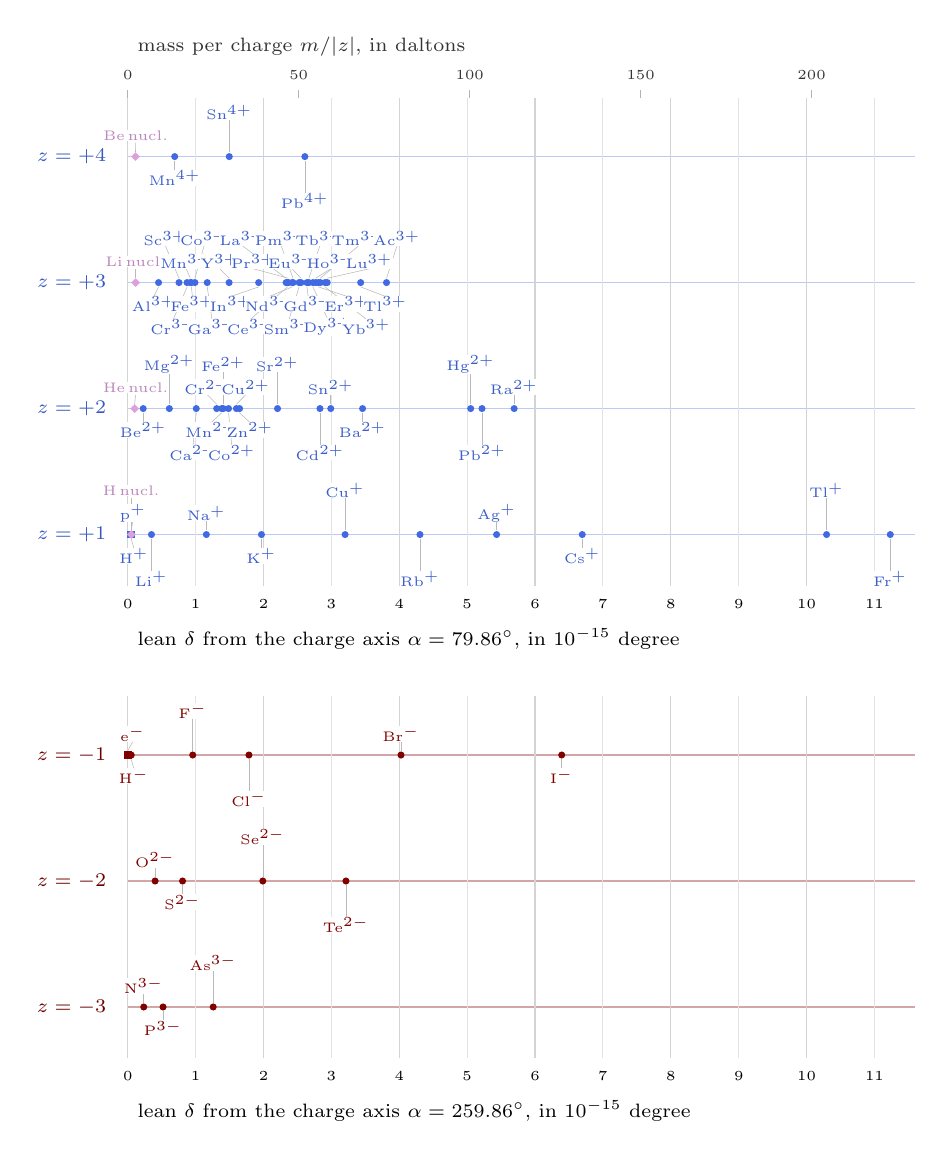
\begin{tikzpicture}[x=1mm, y=1mm, every node/.style={font=\tiny}]
\draw[RoyalBlue!35] (12,0) -- (112,0);
\node[font=\scriptsize, anchor=east, text=RoyalBlue!85!black] at (10.5,0) {$z = +4$};
\draw[RoyalBlue!35] (12,-16) -- (112,-16);
\node[font=\scriptsize, anchor=east, text=RoyalBlue!85!black] at (10.5,-16) {$z = +3$};
\draw[RoyalBlue!35] (12,-32) -- (112,-32);
\node[font=\scriptsize, anchor=east, text=RoyalBlue!85!black] at (10.5,-32) {$z = +2$};
\draw[RoyalBlue!35] (12,-48) -- (112,-48);
\node[font=\scriptsize, anchor=east, text=RoyalBlue!85!black] at (10.5,-48) {$z = +1$};
\draw[Maroon!35] (12,-76) -- (112,-76);
\node[font=\scriptsize, anchor=east, text=Maroon!85!black] at (10.5,-76) {$z = -1$};
\draw[Maroon!35] (12,-92) -- (112,-92);
\node[font=\scriptsize, anchor=east, text=Maroon!85!black] at (10.5,-92) {$z = -2$};
\draw[Maroon!35] (12,-108) -- (112,-108);
\node[font=\scriptsize, anchor=east, text=Maroon!85!black] at (10.5,-108) {$z = -3$};
\draw[gray!34] (12,7.5) -- (12,-54.5);
\draw[gray!22] (20.62,7.5) -- (20.62,-54.5);
\draw[gray!34] (29.24,7.5) -- (29.24,-54.5);
\draw[gray!22] (37.86,7.5) -- (37.86,-54.5);
\draw[gray!34] (46.48,7.5) -- (46.48,-54.5);
\draw[gray!22] (55.1,7.5) -- (55.1,-54.5);
\draw[gray!34] (63.72,7.5) -- (63.72,-54.5);
\draw[gray!22] (72.34,7.5) -- (72.34,-54.5);
\draw[gray!34] (80.97,7.5) -- (80.97,-54.5);
\draw[gray!22] (89.59,7.5) -- (89.59,-54.5);
\draw[gray!34] (98.21,7.5) -- (98.21,-54.5);
\draw[gray!22] (106.83,7.5) -- (106.83,-54.5);
\draw[gray!34] (12,-68.5) -- (12,-114.5);
\draw[gray!22] (20.62,-68.5) -- (20.62,-114.5);
\draw[gray!34] (29.24,-68.5) -- (29.24,-114.5);
\draw[gray!22] (37.86,-68.5) -- (37.86,-114.5);
\draw[gray!34] (46.48,-68.5) -- (46.48,-114.5);
\draw[gray!22] (55.1,-68.5) -- (55.1,-114.5);
\draw[gray!34] (63.72,-68.5) -- (63.72,-114.5);
\draw[gray!22] (72.34,-68.5) -- (72.34,-114.5);
\draw[gray!34] (80.97,-68.5) -- (80.97,-114.5);
\draw[gray!22] (89.59,-68.5) -- (89.59,-114.5);
\draw[gray!34] (98.21,-68.5) -- (98.21,-114.5);
\draw[gray!22] (106.83,-68.5) -- (106.83,-114.5);
\node[anchor=north] at (12,-55) {0};
\node[anchor=north] at (12,-115) {0};
\node[anchor=north] at (20.62,-55) {1};
\node[anchor=north] at (20.62,-115) {1};
\node[anchor=north] at (29.24,-55) {2};
\node[anchor=north] at (29.24,-115) {2};
\node[anchor=north] at (37.86,-55) {3};
\node[anchor=north] at (37.86,-115) {3};
\node[anchor=north] at (46.48,-55) {4};
\node[anchor=north] at (46.48,-115) {4};
\node[anchor=north] at (55.1,-55) {5};
\node[anchor=north] at (55.1,-115) {5};
\node[anchor=north] at (63.72,-55) {6};
\node[anchor=north] at (63.72,-115) {6};
\node[anchor=north] at (72.34,-55) {7};
\node[anchor=north] at (72.34,-115) {7};
\node[anchor=north] at (80.97,-55) {8};
\node[anchor=north] at (80.97,-115) {8};
\node[anchor=north] at (89.59,-55) {9};
\node[anchor=north] at (89.59,-115) {9};
\node[anchor=north] at (98.21,-55) {10};
\node[anchor=north] at (98.21,-115) {10};
\node[anchor=north] at (106.83,-55) {11};
\node[anchor=north] at (106.83,-115) {11};
\draw[gray!60] (12,7.5) -- (12,8.5); \node[anchor=south, text=gray!40!black] at (12,8.5) {0};
\draw[gray!60] (33.71,7.5) -- (33.71,8.5); \node[anchor=south, text=gray!40!black] at (33.71,8.5) {50};
\draw[gray!60] (55.43,7.5) -- (55.43,8.5); \node[anchor=south, text=gray!40!black] at (55.43,8.5) {100};
\draw[gray!60] (77.14,7.5) -- (77.14,8.5); \node[anchor=south, text=gray!40!black] at (77.14,8.5) {150};
\draw[gray!60] (98.85,7.5) -- (98.85,8.5); \node[anchor=south, text=gray!40!black] at (98.85,8.5) {200};
\node[anchor=south west, text=gray!40!black, font=\scriptsize] at (12,11.5) {mass per charge $m/|z|$, in daltons};
\node[anchor=north west, font=\scriptsize] at (12,-58.6) {lean $\delta$ from the charge axis $\alpha = 79.86^\circ$, in $10^{-15}$ degree};
\node[anchor=north west, font=\scriptsize] at (12,-118.6) {lean $\delta$ from the charge axis $\alpha = 259.86^\circ$, in $10^{-15}$ degree};
\draw[gray!55, line width=0.2pt] (12.98,0.55) -- (13,1.75);
\draw[gray!55, line width=0.2pt] (17.96,-0.55) -- (17.96,-1.75);
\draw[gray!55, line width=0.2pt] (24.89,0.55) -- (24.89,4.65);
\draw[gray!55, line width=0.2pt] (34.49,-0.55) -- (34.49,-4.65);
\draw[gray!55, line width=0.2pt] (13,-15.45) -- (13,-14.25);
\draw[gray!55, line width=0.2pt] (19.95,-15.45) -- (19.42,-14.25);
\draw[gray!55, line width=0.2pt] (24.87,-15.45) -- (23.7,-14.25);
\draw[gray!55, line width=0.2pt] (32.4,-15.45) -- (27.97,-14.25);
\draw[gray!55, line width=0.2pt] (34,-15.45) -- (32.87,-14.25);
\draw[gray!55, line width=0.2pt] (35.87,-15.45) -- (37.77,-14.25);
\draw[gray!55, line width=0.2pt] (37.33,-15.45) -- (42.67,-14.25);
\draw[gray!55, line width=0.2pt] (15.91,-16.55) -- (15.31,-17.75);
\draw[gray!55, line width=0.2pt] (20.08,-16.55) -- (20.21,-17.75);
\draw[gray!55, line width=0.2pt] (28.62,-16.55) -- (25.11,-17.75);
\draw[gray!55, line width=0.2pt] (32.88,-16.55) -- (30.01,-17.75);
\draw[gray!55, line width=0.2pt] (34.76,-16.55) -- (34.91,-17.75);
\draw[gray!55, line width=0.2pt] (36.21,-16.55) -- (39.81,-17.75);
\draw[gray!55, line width=0.2pt] (41.58,-16.55) -- (44.71,-17.75);
\draw[gray!55, line width=0.2pt] (18.51,-15.45) -- (16.79,-11.35);
\draw[gray!55, line width=0.2pt] (20.53,-15.45) -- (21.69,-11.35);
\draw[gray!55, line width=0.2pt] (32.11,-15.45) -- (26.59,-11.35);
\draw[gray!55, line width=0.2pt] (32.99,-15.45) -- (31.49,-11.35);
\draw[gray!55, line width=0.2pt] (35,-15.45) -- (36.39,-11.35);
\draw[gray!55, line width=0.2pt] (36.45,-15.45) -- (41.29,-11.35);
\draw[gray!55, line width=0.2pt] (44.86,-15.45) -- (46.19,-11.35);
\draw[gray!55, line width=0.2pt] (19.53,-16.55) -- (17.79,-20.65);
\draw[gray!55, line width=0.2pt] (22.09,-16.55) -- (22.69,-20.65);
\draw[gray!55, line width=0.2pt] (32.28,-16.55) -- (27.59,-20.65);
\draw[gray!55, line width=0.2pt] (33.76,-16.55) -- (32.49,-20.65);
\draw[gray!55, line width=0.2pt] (35.52,-16.55) -- (37.39,-20.65);
\draw[gray!55, line width=0.2pt] (37.05,-16.55) -- (42.29,-20.65);
\draw[gray!55, line width=0.2pt] (12.87,-31.45) -- (13,-30.25);
\draw[gray!55, line width=0.2pt] (23.29,-31.45) -- (22.09,-30.25);
\draw[gray!55, line width=0.2pt] (25.8,-31.45) -- (26.99,-30.25);
\draw[gray!55, line width=0.2pt] (37.78,-31.45) -- (37.78,-30.25);
\draw[gray!55, line width=0.2pt] (61.07,-31.45) -- (61.07,-30.25);
\draw[gray!55, line width=0.2pt] (13.96,-32.55) -- (13.96,-33.75);
\draw[gray!55, line width=0.2pt] (23.93,-32.55) -- (22.61,-33.75);
\draw[gray!55, line width=0.2pt] (26.2,-32.55) -- (27.51,-33.75);
\draw[gray!55, line width=0.2pt] (41.82,-32.55) -- (41.82,-33.75);
\draw[gray!55, line width=0.2pt] (17.28,-31.45) -- (17.28,-27.35);
\draw[gray!55, line width=0.2pt] (24.13,-31.45) -- (24.13,-27.35);
\draw[gray!55, line width=0.2pt] (31.02,-31.45) -- (31.02,-27.35);
\draw[gray!55, line width=0.2pt] (55.55,-31.45) -- (55.55,-27.35);
\draw[gray!55, line width=0.2pt] (20.7,-32.55) -- (20.3,-36.65);
\draw[gray!55, line width=0.2pt] (24.8,-32.55) -- (25.2,-36.65);
\draw[gray!55, line width=0.2pt] (36.41,-32.55) -- (36.41,-36.65);
\draw[gray!55, line width=0.2pt] (56.99,-32.55) -- (56.99,-36.65);
\draw[gray!55, line width=0.2pt] (12.44,-47.45) -- (12.65,-46.25);
\draw[gray!55, line width=0.2pt] (21.98,-47.45) -- (21.98,-46.25);
\draw[gray!55, line width=0.2pt] (58.84,-47.45) -- (58.84,-46.25);
\draw[gray!55, line width=0.2pt] (12.44,-48.55) -- (12.78,-49.75);
\draw[gray!55, line width=0.2pt] (28.98,-48.55) -- (28.98,-49.75);
\draw[gray!55, line width=0.2pt] (69.72,-48.55) -- (69.72,-49.75);
\draw[gray!55, line width=0.2pt] (12.44,-47.45) -- (12.44,-43.35);
\draw[gray!55, line width=0.2pt] (39.6,-47.45) -- (39.6,-43.35);
\draw[gray!55, line width=0.2pt] (100.75,-47.45) -- (100.75,-43.35);
\draw[gray!55, line width=0.2pt] (15.01,-48.55) -- (15.01,-52.65);
\draw[gray!55, line width=0.2pt] (49.11,-48.55) -- (49.11,-52.65);
\draw[gray!55, line width=0.2pt] (108.84,-48.55) -- (108.84,-52.65);
\draw[gray!55, line width=0.2pt] (12,-75.45) -- (12.65,-74.25);
\draw[gray!55, line width=0.2pt] (46.7,-75.45) -- (46.7,-74.25);
\draw[gray!55, line width=0.2pt] (12.44,-76.55) -- (12.78,-77.75);
\draw[gray!55, line width=0.2pt] (67.11,-76.55) -- (67.11,-77.75);
\draw[gray!55, line width=0.2pt] (20.25,-75.45) -- (20.25,-71.35);
\draw[gray!55, line width=0.2pt] (27.39,-76.55) -- (27.39,-80.65);
\draw[gray!55, line width=0.2pt] (15.47,-91.45) -- (15.47,-90.25);
\draw[gray!55, line width=0.2pt] (18.96,-92.55) -- (18.96,-93.75);
\draw[gray!55, line width=0.2pt] (29.15,-91.45) -- (29.15,-87.35);
\draw[gray!55, line width=0.2pt] (39.71,-92.55) -- (39.71,-96.65);
\draw[gray!55, line width=0.2pt] (14.03,-107.45) -- (14.03,-106.25);
\draw[gray!55, line width=0.2pt] (16.48,-108.55) -- (16.48,-109.75);
\draw[gray!55, line width=0.2pt] (22.85,-107.45) -- (22.85,-103.35);
\fill[Plum] (12.98,-0.55) -- ++(0.55,0.55) -- ++(-0.55,0.55) -- ++(-0.55,-0.55) -- cycle;
\fill[RoyalBlue] (17.96,0) circle (0.45);
\fill[RoyalBlue] (24.89,0) circle (0.45);
\fill[RoyalBlue] (34.49,0) circle (0.45);
\fill[Plum] (13,-16.55) -- ++(0.55,0.55) -- ++(-0.55,0.55) -- ++(-0.55,-0.55) -- cycle;
\fill[RoyalBlue] (15.91,-16) circle (0.45);
\fill[RoyalBlue] (18.51,-16) circle (0.45);
\fill[RoyalBlue] (19.53,-16) circle (0.45);
\fill[RoyalBlue] (19.95,-16) circle (0.45);
\fill[RoyalBlue] (20.08,-16) circle (0.45);
\fill[RoyalBlue] (20.53,-16) circle (0.45);
\fill[RoyalBlue] (22.09,-16) circle (0.45);
\fill[RoyalBlue] (24.87,-16) circle (0.45);
\fill[RoyalBlue] (28.62,-16) circle (0.45);
\fill[RoyalBlue] (32.11,-16) circle (0.45);
\fill[RoyalBlue] (32.28,-16) circle (0.45);
\fill[RoyalBlue] (32.4,-16) circle (0.45);
\fill[RoyalBlue] (32.88,-16) circle (0.45);
\fill[RoyalBlue] (32.99,-16) circle (0.45);
\fill[RoyalBlue] (33.76,-16) circle (0.45);
\fill[RoyalBlue] (34,-16) circle (0.45);
\fill[RoyalBlue] (34.76,-16) circle (0.45);
\fill[RoyalBlue] (35,-16) circle (0.45);
\fill[RoyalBlue] (35.52,-16) circle (0.45);
\fill[RoyalBlue] (35.87,-16) circle (0.45);
\fill[RoyalBlue] (36.21,-16) circle (0.45);
\fill[RoyalBlue] (36.45,-16) circle (0.45);
\fill[RoyalBlue] (37.05,-16) circle (0.45);
\fill[RoyalBlue] (37.33,-16) circle (0.45);
\fill[RoyalBlue] (41.58,-16) circle (0.45);
\fill[RoyalBlue] (44.86,-16) circle (0.45);
\fill[Plum] (12.87,-32.55) -- ++(0.55,0.55) -- ++(-0.55,0.55) -- ++(-0.55,-0.55) -- cycle;
\fill[RoyalBlue] (13.96,-32) circle (0.45);
\fill[RoyalBlue] (17.28,-32) circle (0.45);
\fill[RoyalBlue] (20.7,-32) circle (0.45);
\fill[RoyalBlue] (23.29,-32) circle (0.45);
\fill[RoyalBlue] (23.93,-32) circle (0.45);
\fill[RoyalBlue] (24.13,-32) circle (0.45);
\fill[RoyalBlue] (24.8,-32) circle (0.45);
\fill[RoyalBlue] (25.8,-32) circle (0.45);
\fill[RoyalBlue] (26.2,-32) circle (0.45);
\fill[RoyalBlue] (31.02,-32) circle (0.45);
\fill[RoyalBlue] (36.41,-32) circle (0.45);
\fill[RoyalBlue] (37.78,-32) circle (0.45);
\fill[RoyalBlue] (41.82,-32) circle (0.45);
\fill[RoyalBlue] (55.55,-32) circle (0.45);
\fill[RoyalBlue] (56.99,-32) circle (0.45);
\fill[RoyalBlue] (61.07,-32) circle (0.45);
\fill[RoyalBlue] (11.94,-48.5) rectangle (12.94,-47.5);
\fill[RoyalBlue] (12.44,-48) circle (0.45);
\fill[Plum] (12.44,-48.55) -- ++(0.55,0.55) -- ++(-0.55,0.55) -- ++(-0.55,-0.55) -- cycle;
\fill[RoyalBlue] (15.01,-48) circle (0.45);
\fill[RoyalBlue] (21.98,-48) circle (0.45);
\fill[RoyalBlue] (28.98,-48) circle (0.45);
\fill[RoyalBlue] (39.6,-48) circle (0.45);
\fill[RoyalBlue] (49.11,-48) circle (0.45);
\fill[RoyalBlue] (58.84,-48) circle (0.45);
\fill[RoyalBlue] (69.72,-48) circle (0.45);
\fill[RoyalBlue] (100.75,-48) circle (0.45);
\fill[RoyalBlue] (108.84,-48) circle (0.45);
\fill[Maroon] (11.5,-76.5) rectangle (12.5,-75.5);
\fill[Maroon] (12.44,-76) circle (0.45);
\fill[Maroon] (20.25,-76) circle (0.45);
\fill[Maroon] (27.39,-76) circle (0.45);
\fill[Maroon] (46.7,-76) circle (0.45);
\fill[Maroon] (67.11,-76) circle (0.45);
\fill[Maroon] (15.47,-92) circle (0.45);
\fill[Maroon] (18.96,-92) circle (0.45);
\fill[Maroon] (29.15,-92) circle (0.45);
\fill[Maroon] (39.71,-92) circle (0.45);
\fill[Maroon] (14.03,-108) circle (0.45);
\fill[Maroon] (16.48,-108) circle (0.45);
\fill[Maroon] (22.85,-108) circle (0.45);
\node[text=Plum!85!black, fill=white, inner sep=0.15pt] at (13,2.7) {Be\,nucl.};
\node[text=RoyalBlue!90!black, fill=white, inner sep=0.15pt] at (17.96,-2.7) {Mn$^{4+}$};
\node[text=RoyalBlue!90!black, fill=white, inner sep=0.15pt] at (24.89,5.6) {Sn$^{4+}$};
\node[text=RoyalBlue!90!black, fill=white, inner sep=0.15pt] at (34.49,-5.6) {Pb$^{4+}$};
\node[text=Plum!85!black, fill=white, inner sep=0.15pt] at (13,-13.3) {Li\,nucl.};
\node[text=RoyalBlue!90!black, fill=white, inner sep=0.15pt] at (19.42,-13.3) {Mn$^{3+}$};
\node[text=RoyalBlue!90!black, fill=white, inner sep=0.15pt] at (23.7,-13.3) {Y$^{3+}$};
\node[text=RoyalBlue!90!black, fill=white, inner sep=0.15pt] at (27.97,-13.3) {Pr$^{3+}$};
\node[text=RoyalBlue!90!black, fill=white, inner sep=0.15pt] at (32.87,-13.3) {Eu$^{3+}$};
\node[text=RoyalBlue!90!black, fill=white, inner sep=0.15pt] at (37.77,-13.3) {Ho$^{3+}$};
\node[text=RoyalBlue!90!black, fill=white, inner sep=0.15pt] at (42.67,-13.3) {Lu$^{3+}$};
\node[text=RoyalBlue!90!black, fill=white, inner sep=0.15pt] at (15.31,-18.7) {Al$^{3+}$};
\node[text=RoyalBlue!90!black, fill=white, inner sep=0.15pt] at (20.21,-18.7) {Fe$^{3+}$};
\node[text=RoyalBlue!90!black, fill=white, inner sep=0.15pt] at (25.11,-18.7) {In$^{3+}$};
\node[text=RoyalBlue!90!black, fill=white, inner sep=0.15pt] at (30.01,-18.7) {Nd$^{3+}$};
\node[text=RoyalBlue!90!black, fill=white, inner sep=0.15pt] at (34.91,-18.7) {Gd$^{3+}$};
\node[text=RoyalBlue!90!black, fill=white, inner sep=0.15pt] at (39.81,-18.7) {Er$^{3+}$};
\node[text=RoyalBlue!90!black, fill=white, inner sep=0.15pt] at (44.71,-18.7) {Tl$^{3+}$};
\node[text=RoyalBlue!90!black, fill=white, inner sep=0.15pt] at (16.79,-10.4) {Sc$^{3+}$};
\node[text=RoyalBlue!90!black, fill=white, inner sep=0.15pt] at (21.69,-10.4) {Co$^{3+}$};
\node[text=RoyalBlue!90!black, fill=white, inner sep=0.15pt] at (26.59,-10.4) {La$^{3+}$};
\node[text=RoyalBlue!90!black, fill=white, inner sep=0.15pt] at (31.49,-10.4) {Pm$^{3+}$};
\node[text=RoyalBlue!90!black, fill=white, inner sep=0.15pt] at (36.39,-10.4) {Tb$^{3+}$};
\node[text=RoyalBlue!90!black, fill=white, inner sep=0.15pt] at (41.29,-10.4) {Tm$^{3+}$};
\node[text=RoyalBlue!90!black, fill=white, inner sep=0.15pt] at (46.19,-10.4) {Ac$^{3+}$};
\node[text=RoyalBlue!90!black, fill=white, inner sep=0.15pt] at (17.79,-21.6) {Cr$^{3+}$};
\node[text=RoyalBlue!90!black, fill=white, inner sep=0.15pt] at (22.69,-21.6) {Ga$^{3+}$};
\node[text=RoyalBlue!90!black, fill=white, inner sep=0.15pt] at (27.59,-21.6) {Ce$^{3+}$};
\node[text=RoyalBlue!90!black, fill=white, inner sep=0.15pt] at (32.49,-21.6) {Sm$^{3+}$};
\node[text=RoyalBlue!90!black, fill=white, inner sep=0.15pt] at (37.39,-21.6) {Dy$^{3+}$};
\node[text=RoyalBlue!90!black, fill=white, inner sep=0.15pt] at (42.29,-21.6) {Yb$^{3+}$};
\node[text=Plum!85!black, fill=white, inner sep=0.15pt] at (13,-29.3) {He\,nucl.};
\node[text=RoyalBlue!90!black, fill=white, inner sep=0.15pt] at (22.09,-29.3) {Cr$^{2+}$};
\node[text=RoyalBlue!90!black, fill=white, inner sep=0.15pt] at (26.99,-29.3) {Cu$^{2+}$};
\node[text=RoyalBlue!90!black, fill=white, inner sep=0.15pt] at (37.78,-29.3) {Sn$^{2+}$};
\node[text=RoyalBlue!90!black, fill=white, inner sep=0.15pt] at (61.07,-29.3) {Ra$^{2+}$};
\node[text=RoyalBlue!90!black, fill=white, inner sep=0.15pt] at (13.96,-34.7) {Be$^{2+}$};
\node[text=RoyalBlue!90!black, fill=white, inner sep=0.15pt] at (22.61,-34.7) {Mn$^{2+}$};
\node[text=RoyalBlue!90!black, fill=white, inner sep=0.15pt] at (27.51,-34.7) {Zn$^{2+}$};
\node[text=RoyalBlue!90!black, fill=white, inner sep=0.15pt] at (41.82,-34.7) {Ba$^{2+}$};
\node[text=RoyalBlue!90!black, fill=white, inner sep=0.15pt] at (17.28,-26.4) {Mg$^{2+}$};
\node[text=RoyalBlue!90!black, fill=white, inner sep=0.15pt] at (24.13,-26.4) {Fe$^{2+}$};
\node[text=RoyalBlue!90!black, fill=white, inner sep=0.15pt] at (31.02,-26.4) {Sr$^{2+}$};
\node[text=RoyalBlue!90!black, fill=white, inner sep=0.15pt] at (55.55,-26.4) {Hg$^{2+}$};
\node[text=RoyalBlue!90!black, fill=white, inner sep=0.15pt] at (20.3,-37.6) {Ca$^{2+}$};
\node[text=RoyalBlue!90!black, fill=white, inner sep=0.15pt] at (25.2,-37.6) {Co$^{2+}$};
\node[text=RoyalBlue!90!black, fill=white, inner sep=0.15pt] at (36.41,-37.6) {Cd$^{2+}$};
\node[text=RoyalBlue!90!black, fill=white, inner sep=0.15pt] at (56.99,-37.6) {Pb$^{2+}$};
\node[text=RoyalBlue!90!black, fill=white, inner sep=0.15pt] at (12.65,-45.3) {p$^+$};
\node[text=RoyalBlue!90!black, fill=white, inner sep=0.15pt] at (21.98,-45.3) {Na$^{+}$};
\node[text=RoyalBlue!90!black, fill=white, inner sep=0.15pt] at (58.84,-45.3) {Ag$^{+}$};
\node[text=RoyalBlue!90!black, fill=white, inner sep=0.15pt] at (12.78,-50.7) {H$^{+}$};
\node[text=RoyalBlue!90!black, fill=white, inner sep=0.15pt] at (28.98,-50.7) {K$^{+}$};
\node[text=RoyalBlue!90!black, fill=white, inner sep=0.15pt] at (69.72,-50.7) {Cs$^{+}$};
\node[text=Plum!85!black, fill=white, inner sep=0.15pt] at (12.44,-42.4) {H\,nucl.};
\node[text=RoyalBlue!90!black, fill=white, inner sep=0.15pt] at (39.6,-42.4) {Cu$^{+}$};
\node[text=RoyalBlue!90!black, fill=white, inner sep=0.15pt] at (100.75,-42.4) {Tl$^{+}$};
\node[text=RoyalBlue!90!black, fill=white, inner sep=0.15pt] at (15.01,-53.6) {Li$^{+}$};
\node[text=RoyalBlue!90!black, fill=white, inner sep=0.15pt] at (49.11,-53.6) {Rb$^{+}$};
\node[text=RoyalBlue!90!black, fill=white, inner sep=0.15pt] at (108.84,-53.6) {Fr$^{+}$};
\node[text=Maroon, fill=white, inner sep=0.15pt] at (12.65,-73.3) {e$^-$};
\node[text=Maroon, fill=white, inner sep=0.15pt] at (46.7,-73.3) {Br$^{-}$};
\node[text=Maroon, fill=white, inner sep=0.15pt] at (12.78,-78.7) {H$^{-}$};
\node[text=Maroon, fill=white, inner sep=0.15pt] at (67.11,-78.7) {I$^{-}$};
\node[text=Maroon, fill=white, inner sep=0.15pt] at (20.25,-70.4) {F$^{-}$};
\node[text=Maroon, fill=white, inner sep=0.15pt] at (27.39,-81.6) {Cl$^{-}$};
\node[text=Maroon, fill=white, inner sep=0.15pt] at (15.47,-89.3) {O$^{2-}$};
\node[text=Maroon, fill=white, inner sep=0.15pt] at (18.96,-94.7) {S$^{2-}$};
\node[text=Maroon, fill=white, inner sep=0.15pt] at (29.15,-86.4) {Se$^{2-}$};
\node[text=Maroon, fill=white, inner sep=0.15pt] at (39.71,-97.6) {Te$^{2-}$};
\node[text=Maroon, fill=white, inner sep=0.15pt] at (14.03,-105.3) {N$^{3-}$};
\node[text=Maroon, fill=white, inner sep=0.15pt] at (16.48,-110.7) {P$^{3-}$};
\node[text=Maroon, fill=white, inner sep=0.15pt] at (22.85,-102.4) {As$^{3-}$};
\end{tikzpicture}
}
\caption[The ions, every one named]{The ions of \Cref{fig:standard-model}, every one named. The two magnified sectors next to the charge axis are unrolled: each ring $z$ becomes a line, and the lean $\delta$ runs across, in $10^{-15}$ degree, from the charge axis on the left. The scale on top reads the same lean as mass per charge. Blue: cations and the proton (square); red: anions and the electron (square); violet: the bare nuclei of hydrogen to beryllium, which share the rings $1$ to $4$ with the ions.}
\label{fig:sm-ions}
\end{figure}

\begin{figure}[p]
\myfloatalign
\makebox[\textwidth][c]{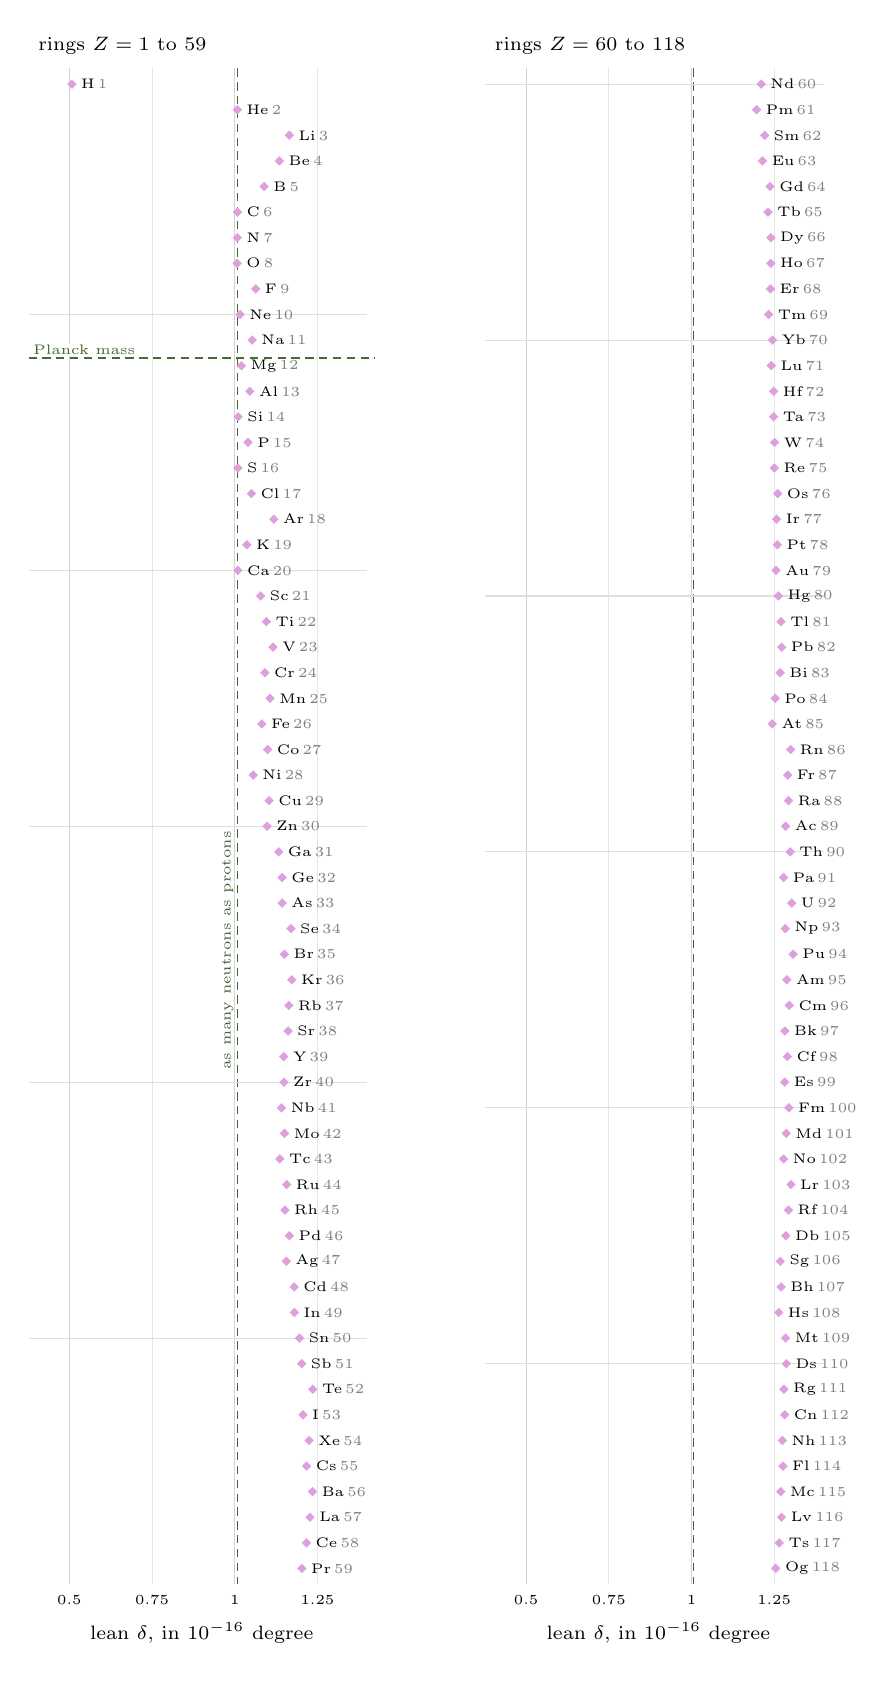
\begin{tikzpicture}[x=1mm, y=1mm, every node/.style={font=\tiny}]
\draw[gray!35] (4.2,2) -- (4.2,-190.5);
\node[anchor=north] at (4.2,-190.7) {0.5};
\draw[gray!20] (14.7,2) -- (14.7,-190.5);
\node[anchor=north] at (14.7,-190.7) {0.75};
\draw[gray!35] (25.2,2) -- (25.2,-190.5);
\node[anchor=north] at (25.2,-190.7) {1};
\draw[gray!20] (35.7,2) -- (35.7,-190.5);
\node[anchor=north] at (35.7,-190.7) {1.25};
\draw[OliveGreen!70!black, densely dashed] (25.51,2) -- (25.51,-190.5);
\node[anchor=north, align=center, font=\scriptsize] at (21,-194.1) {lean $\delta$, in $10^{-16}$ degree};
\draw[gray!25] (-1,-29.25) -- (42,-29.25);
\draw[gray!25] (-1,-61.75) -- (42,-61.75);
\draw[gray!25] (-1,-94.25) -- (42,-94.25);
\draw[gray!25] (-1,-126.75) -- (42,-126.75);
\draw[gray!25] (-1,-159.25) -- (42,-159.25);
\fill[Plum] (4.51,-0.6) -- ++(0.6,0.6) -- ++(-0.6,0.6) -- ++(-0.6,-0.6) -- cycle;
\node[anchor=west, inner sep=0.3pt] at (5.51,0) {H\,\textcolor{gray}{1}};
\fill[Plum] (25.53,-3.85) -- ++(0.6,0.6) -- ++(-0.6,0.6) -- ++(-0.6,-0.6) -- cycle;
\node[anchor=west, inner sep=0.3pt] at (26.53,-3.25) {He\,\textcolor{gray}{2}};
\fill[Plum] (32.13,-7.1) -- ++(0.6,0.6) -- ++(-0.6,0.6) -- ++(-0.6,-0.6) -- cycle;
\node[anchor=west, inner sep=0.3pt] at (33.13,-6.5) {Li\,\textcolor{gray}{3}};
\fill[Plum] (30.86,-10.35) -- ++(0.6,0.6) -- ++(-0.6,0.6) -- ++(-0.6,-0.6) -- cycle;
\node[anchor=west, inner sep=0.3pt] at (31.86,-9.75) {Be\,\textcolor{gray}{4}};
\fill[Plum] (28.93,-13.6) -- ++(0.6,0.6) -- ++(-0.6,0.6) -- ++(-0.6,-0.6) -- cycle;
\node[anchor=west, inner sep=0.3pt] at (29.93,-13) {B\,\textcolor{gray}{5}};
\fill[Plum] (25.54,-16.85) -- ++(0.6,0.6) -- ++(-0.6,0.6) -- ++(-0.6,-0.6) -- cycle;
\node[anchor=west, inner sep=0.3pt] at (26.54,-16.25) {C\,\textcolor{gray}{6}};
\fill[Plum] (25.52,-20.1) -- ++(0.6,0.6) -- ++(-0.6,0.6) -- ++(-0.6,-0.6) -- cycle;
\node[anchor=west, inner sep=0.3pt] at (26.52,-19.5) {N\,\textcolor{gray}{7}};
\fill[Plum] (25.5,-23.35) -- ++(0.6,0.6) -- ++(-0.6,0.6) -- ++(-0.6,-0.6) -- cycle;
\node[anchor=west, inner sep=0.3pt] at (26.5,-22.75) {O\,\textcolor{gray}{8}};
\fill[Plum] (27.85,-26.6) -- ++(0.6,0.6) -- ++(-0.6,0.6) -- ++(-0.6,-0.6) -- cycle;
\node[anchor=west, inner sep=0.3pt] at (28.85,-26) {F\,\textcolor{gray}{9}};
\fill[Plum] (25.88,-29.85) -- ++(0.6,0.6) -- ++(-0.6,0.6) -- ++(-0.6,-0.6) -- cycle;
\node[anchor=west, inner sep=0.3pt] at (26.88,-29.25) {Ne\,\textcolor{gray}{10}};
\fill[Plum] (27.41,-33.1) -- ++(0.6,0.6) -- ++(-0.6,0.6) -- ++(-0.6,-0.6) -- cycle;
\node[anchor=west, inner sep=0.3pt] at (28.41,-32.5) {Na\,\textcolor{gray}{11}};
\fill[Plum] (26.04,-36.35) -- ++(0.6,0.6) -- ++(-0.6,0.6) -- ++(-0.6,-0.6) -- cycle;
\node[anchor=west, inner sep=0.3pt] at (27.04,-35.75) {Mg\,\textcolor{gray}{12}};
\fill[Plum] (27.1,-39.6) -- ++(0.6,0.6) -- ++(-0.6,0.6) -- ++(-0.6,-0.6) -- cycle;
\node[anchor=west, inner sep=0.3pt] at (28.1,-39) {Al\,\textcolor{gray}{13}};
\fill[Plum] (25.63,-42.85) -- ++(0.6,0.6) -- ++(-0.6,0.6) -- ++(-0.6,-0.6) -- cycle;
\node[anchor=west, inner sep=0.3pt] at (26.63,-42.25) {Si\,\textcolor{gray}{14}};
\fill[Plum] (26.88,-46.1) -- ++(0.6,0.6) -- ++(-0.6,0.6) -- ++(-0.6,-0.6) -- cycle;
\node[anchor=west, inner sep=0.3pt] at (27.88,-45.5) {P\,\textcolor{gray}{15}};
\fill[Plum] (25.58,-49.35) -- ++(0.6,0.6) -- ++(-0.6,0.6) -- ++(-0.6,-0.6) -- cycle;
\node[anchor=west, inner sep=0.3pt] at (26.58,-48.75) {S\,\textcolor{gray}{16}};
\fill[Plum] (27.31,-52.6) -- ++(0.6,0.6) -- ++(-0.6,0.6) -- ++(-0.6,-0.6) -- cycle;
\node[anchor=west, inner sep=0.3pt] at (28.31,-52) {Cl\,\textcolor{gray}{17}};
\fill[Plum] (30.15,-55.85) -- ++(0.6,0.6) -- ++(-0.6,0.6) -- ++(-0.6,-0.6) -- cycle;
\node[anchor=west, inner sep=0.3pt] at (31.15,-55.25) {Ar\,\textcolor{gray}{18}};
\fill[Plum] (26.73,-59.1) -- ++(0.6,0.6) -- ++(-0.6,0.6) -- ++(-0.6,-0.6) -- cycle;
\node[anchor=west, inner sep=0.3pt] at (27.73,-58.5) {K\,\textcolor{gray}{19}};
\fill[Plum] (25.59,-62.35) -- ++(0.6,0.6) -- ++(-0.6,0.6) -- ++(-0.6,-0.6) -- cycle;
\node[anchor=west, inner sep=0.3pt] at (26.59,-61.75) {Ca\,\textcolor{gray}{20}};
\fill[Plum] (28.48,-65.6) -- ++(0.6,0.6) -- ++(-0.6,0.6) -- ++(-0.6,-0.6) -- cycle;
\node[anchor=west, inner sep=0.3pt] at (29.48,-65) {Sc\,\textcolor{gray}{21}};
\fill[Plum] (29.22,-68.85) -- ++(0.6,0.6) -- ++(-0.6,0.6) -- ++(-0.6,-0.6) -- cycle;
\node[anchor=west, inner sep=0.3pt] at (30.22,-68.25) {Ti\,\textcolor{gray}{22}};
\fill[Plum] (30.05,-72.1) -- ++(0.6,0.6) -- ++(-0.6,0.6) -- ++(-0.6,-0.6) -- cycle;
\node[anchor=west, inner sep=0.3pt] at (31.05,-71.5) {V\,\textcolor{gray}{23}};
\fill[Plum] (29.03,-75.35) -- ++(0.6,0.6) -- ++(-0.6,0.6) -- ++(-0.6,-0.6) -- cycle;
\node[anchor=west, inner sep=0.3pt] at (30.03,-74.75) {Cr\,\textcolor{gray}{24}};
\fill[Plum] (29.68,-78.6) -- ++(0.6,0.6) -- ++(-0.6,0.6) -- ++(-0.6,-0.6) -- cycle;
\node[anchor=west, inner sep=0.3pt] at (30.68,-78) {Mn\,\textcolor{gray}{25}};
\fill[Plum] (28.63,-81.85) -- ++(0.6,0.6) -- ++(-0.6,0.6) -- ++(-0.6,-0.6) -- cycle;
\node[anchor=west, inner sep=0.3pt] at (29.63,-81.25) {Fe\,\textcolor{gray}{26}};
\fill[Plum] (29.37,-85.1) -- ++(0.6,0.6) -- ++(-0.6,0.6) -- ++(-0.6,-0.6) -- cycle;
\node[anchor=west, inner sep=0.3pt] at (30.37,-84.5) {Co\,\textcolor{gray}{27}};
\fill[Plum] (27.54,-88.35) -- ++(0.6,0.6) -- ++(-0.6,0.6) -- ++(-0.6,-0.6) -- cycle;
\node[anchor=west, inner sep=0.3pt] at (28.54,-87.75) {Ni\,\textcolor{gray}{28}};
\fill[Plum] (29.55,-91.6) -- ++(0.6,0.6) -- ++(-0.6,0.6) -- ++(-0.6,-0.6) -- cycle;
\node[anchor=west, inner sep=0.3pt] at (30.55,-91) {Cu\,\textcolor{gray}{29}};
\fill[Plum] (29.3,-94.85) -- ++(0.6,0.6) -- ++(-0.6,0.6) -- ++(-0.6,-0.6) -- cycle;
\node[anchor=west, inner sep=0.3pt] at (30.3,-94.25) {Zn\,\textcolor{gray}{30}};
\fill[Plum] (30.77,-98.1) -- ++(0.6,0.6) -- ++(-0.6,0.6) -- ++(-0.6,-0.6) -- cycle;
\node[anchor=west, inner sep=0.3pt] at (31.77,-97.5) {Ga\,\textcolor{gray}{31}};
\fill[Plum] (31.21,-101.35) -- ++(0.6,0.6) -- ++(-0.6,0.6) -- ++(-0.6,-0.6) -- cycle;
\node[anchor=west, inner sep=0.3pt] at (32.21,-100.75) {Ge\,\textcolor{gray}{32}};
\fill[Plum] (31.22,-104.6) -- ++(0.6,0.6) -- ++(-0.6,0.6) -- ++(-0.6,-0.6) -- cycle;
\node[anchor=west, inner sep=0.3pt] at (32.22,-104) {As\,\textcolor{gray}{33}};
\fill[Plum] (32.33,-107.85) -- ++(0.6,0.6) -- ++(-0.6,0.6) -- ++(-0.6,-0.6) -- cycle;
\node[anchor=west, inner sep=0.3pt] at (33.33,-107.25) {Se\,\textcolor{gray}{34}};
\fill[Plum] (31.49,-111.1) -- ++(0.6,0.6) -- ++(-0.6,0.6) -- ++(-0.6,-0.6) -- cycle;
\node[anchor=west, inner sep=0.3pt] at (32.49,-110.5) {Br\,\textcolor{gray}{35}};
\fill[Plum] (32.44,-114.35) -- ++(0.6,0.6) -- ++(-0.6,0.6) -- ++(-0.6,-0.6) -- cycle;
\node[anchor=west, inner sep=0.3pt] at (33.44,-113.75) {Kr\,\textcolor{gray}{36}};
\fill[Plum] (32.06,-117.6) -- ++(0.6,0.6) -- ++(-0.6,0.6) -- ++(-0.6,-0.6) -- cycle;
\node[anchor=west, inner sep=0.3pt] at (33.06,-117) {Rb\,\textcolor{gray}{37}};
\fill[Plum] (31.97,-120.85) -- ++(0.6,0.6) -- ++(-0.6,0.6) -- ++(-0.6,-0.6) -- cycle;
\node[anchor=west, inner sep=0.3pt] at (32.97,-120.25) {Sr\,\textcolor{gray}{38}};
\fill[Plum] (31.42,-124.1) -- ++(0.6,0.6) -- ++(-0.6,0.6) -- ++(-0.6,-0.6) -- cycle;
\node[anchor=west, inner sep=0.3pt] at (32.42,-123.5) {Y\,\textcolor{gray}{39}};
\fill[Plum] (31.44,-127.35) -- ++(0.6,0.6) -- ++(-0.6,0.6) -- ++(-0.6,-0.6) -- cycle;
\node[anchor=west, inner sep=0.3pt] at (32.44,-126.75) {Zr\,\textcolor{gray}{40}};
\fill[Plum] (31.13,-130.6) -- ++(0.6,0.6) -- ++(-0.6,0.6) -- ++(-0.6,-0.6) -- cycle;
\node[anchor=west, inner sep=0.3pt] at (32.13,-130) {Nb\,\textcolor{gray}{41}};
\fill[Plum] (31.52,-133.85) -- ++(0.6,0.6) -- ++(-0.6,0.6) -- ++(-0.6,-0.6) -- cycle;
\node[anchor=west, inner sep=0.3pt] at (32.52,-133.25) {Mo\,\textcolor{gray}{42}};
\fill[Plum] (30.91,-137.1) -- ++(0.6,0.6) -- ++(-0.6,0.6) -- ++(-0.6,-0.6) -- cycle;
\node[anchor=west, inner sep=0.3pt] at (31.91,-136.5) {Tc\,\textcolor{gray}{43}};
\fill[Plum] (31.79,-140.35) -- ++(0.6,0.6) -- ++(-0.6,0.6) -- ++(-0.6,-0.6) -- cycle;
\node[anchor=west, inner sep=0.3pt] at (32.79,-139.75) {Ru\,\textcolor{gray}{44}};
\fill[Plum] (31.57,-143.6) -- ++(0.6,0.6) -- ++(-0.6,0.6) -- ++(-0.6,-0.6) -- cycle;
\node[anchor=west, inner sep=0.3pt] at (32.57,-143) {Rh\,\textcolor{gray}{45}};
\fill[Plum] (32.13,-146.85) -- ++(0.6,0.6) -- ++(-0.6,0.6) -- ++(-0.6,-0.6) -- cycle;
\node[anchor=west, inner sep=0.3pt] at (33.13,-146.25) {Pd\,\textcolor{gray}{46}};
\fill[Plum] (31.75,-150.1) -- ++(0.6,0.6) -- ++(-0.6,0.6) -- ++(-0.6,-0.6) -- cycle;
\node[anchor=west, inner sep=0.3pt] at (32.75,-149.5) {Ag\,\textcolor{gray}{47}};
\fill[Plum] (32.74,-153.35) -- ++(0.6,0.6) -- ++(-0.6,0.6) -- ++(-0.6,-0.6) -- cycle;
\node[anchor=west, inner sep=0.3pt] at (33.74,-152.75) {Cd\,\textcolor{gray}{48}};
\fill[Plum] (32.76,-156.6) -- ++(0.6,0.6) -- ++(-0.6,0.6) -- ++(-0.6,-0.6) -- cycle;
\node[anchor=west, inner sep=0.3pt] at (33.76,-156) {In\,\textcolor{gray}{49}};
\fill[Plum] (33.42,-159.85) -- ++(0.6,0.6) -- ++(-0.6,0.6) -- ++(-0.6,-0.6) -- cycle;
\node[anchor=west, inner sep=0.3pt] at (34.42,-159.25) {Sn\,\textcolor{gray}{50}};
\fill[Plum] (33.7,-163.1) -- ++(0.6,0.6) -- ++(-0.6,0.6) -- ++(-0.6,-0.6) -- cycle;
\node[anchor=west, inner sep=0.3pt] at (34.7,-162.5) {Sb\,\textcolor{gray}{51}};
\fill[Plum] (35.1,-166.35) -- ++(0.6,0.6) -- ++(-0.6,0.6) -- ++(-0.6,-0.6) -- cycle;
\node[anchor=west, inner sep=0.3pt] at (36.1,-165.75) {Te\,\textcolor{gray}{52}};
\fill[Plum] (33.85,-169.6) -- ++(0.6,0.6) -- ++(-0.6,0.6) -- ++(-0.6,-0.6) -- cycle;
\node[anchor=west, inner sep=0.3pt] at (34.85,-169) {I\,\textcolor{gray}{53}};
\fill[Plum] (34.63,-172.85) -- ++(0.6,0.6) -- ++(-0.6,0.6) -- ++(-0.6,-0.6) -- cycle;
\node[anchor=west, inner sep=0.3pt] at (35.63,-172.25) {Xe\,\textcolor{gray}{54}};
\fill[Plum] (34.31,-176.1) -- ++(0.6,0.6) -- ++(-0.6,0.6) -- ++(-0.6,-0.6) -- cycle;
\node[anchor=west, inner sep=0.3pt] at (35.31,-175.5) {Cs\,\textcolor{gray}{55}};
\fill[Plum] (35.07,-179.35) -- ++(0.6,0.6) -- ++(-0.6,0.6) -- ++(-0.6,-0.6) -- cycle;
\node[anchor=west, inner sep=0.3pt] at (36.07,-178.75) {Ba\,\textcolor{gray}{56}};
\fill[Plum] (34.75,-182.6) -- ++(0.6,0.6) -- ++(-0.6,0.6) -- ++(-0.6,-0.6) -- cycle;
\node[anchor=west, inner sep=0.3pt] at (35.75,-182) {La\,\textcolor{gray}{57}};
\fill[Plum] (34.3,-185.85) -- ++(0.6,0.6) -- ++(-0.6,0.6) -- ++(-0.6,-0.6) -- cycle;
\node[anchor=west, inner sep=0.3pt] at (35.3,-185.25) {Ce\,\textcolor{gray}{58}};
\fill[Plum] (33.72,-189.1) -- ++(0.6,0.6) -- ++(-0.6,0.6) -- ++(-0.6,-0.6) -- cycle;
\node[anchor=west, inner sep=0.3pt] at (34.72,-188.5) {Pr\,\textcolor{gray}{59}};
\node[anchor=south west, font=\scriptsize] at (-1,2.6) {rings $Z = 1$ to $59$};
\draw[gray!35] (62.2,2) -- (62.2,-190.5);
\node[anchor=north] at (62.2,-190.7) {0.5};
\draw[gray!20] (72.7,2) -- (72.7,-190.5);
\node[anchor=north] at (72.7,-190.7) {0.75};
\draw[gray!35] (83.2,2) -- (83.2,-190.5);
\node[anchor=north] at (83.2,-190.7) {1};
\draw[gray!20] (93.7,2) -- (93.7,-190.5);
\node[anchor=north] at (93.7,-190.7) {1.25};
\draw[OliveGreen!70!black, densely dashed] (83.51,2) -- (83.51,-190.5);
\node[anchor=north, align=center, font=\scriptsize] at (79,-194.1) {lean $\delta$, in $10^{-16}$ degree};
\draw[gray!25] (57,0) -- (100,0);
\draw[gray!25] (57,-32.5) -- (100,-32.5);
\draw[gray!25] (57,-65) -- (100,-65);
\draw[gray!25] (57,-97.5) -- (100,-97.5);
\draw[gray!25] (57,-130) -- (100,-130);
\draw[gray!25] (57,-162.5) -- (100,-162.5);
\fill[Plum] (92.05,-0.6) -- ++(0.6,0.6) -- ++(-0.6,0.6) -- ++(-0.6,-0.6) -- cycle;
\node[anchor=west, inner sep=0.3pt] at (93.05,0) {Nd\,\textcolor{gray}{60}};
\fill[Plum] (91.48,-3.85) -- ++(0.6,0.6) -- ++(-0.6,0.6) -- ++(-0.6,-0.6) -- cycle;
\node[anchor=west, inner sep=0.3pt] at (92.48,-3.25) {Pm\,\textcolor{gray}{61}};
\fill[Plum] (92.5,-7.1) -- ++(0.6,0.6) -- ++(-0.6,0.6) -- ++(-0.6,-0.6) -- cycle;
\node[anchor=west, inner sep=0.3pt] at (93.5,-6.5) {Sm\,\textcolor{gray}{62}};
\fill[Plum] (92.22,-10.35) -- ++(0.6,0.6) -- ++(-0.6,0.6) -- ++(-0.6,-0.6) -- cycle;
\node[anchor=west, inner sep=0.3pt] at (93.22,-9.75) {Eu\,\textcolor{gray}{63}};
\fill[Plum] (93.17,-13.6) -- ++(0.6,0.6) -- ++(-0.6,0.6) -- ++(-0.6,-0.6) -- cycle;
\node[anchor=west, inner sep=0.3pt] at (94.17,-13) {Gd\,\textcolor{gray}{64}};
\fill[Plum] (92.92,-16.85) -- ++(0.6,0.6) -- ++(-0.6,0.6) -- ++(-0.6,-0.6) -- cycle;
\node[anchor=west, inner sep=0.3pt] at (93.92,-16.25) {Tb\,\textcolor{gray}{65}};
\fill[Plum] (93.28,-20.1) -- ++(0.6,0.6) -- ++(-0.6,0.6) -- ++(-0.6,-0.6) -- cycle;
\node[anchor=west, inner sep=0.3pt] at (94.28,-19.5) {Dy\,\textcolor{gray}{66}};
\fill[Plum] (93.27,-23.35) -- ++(0.6,0.6) -- ++(-0.6,0.6) -- ++(-0.6,-0.6) -- cycle;
\node[anchor=west, inner sep=0.3pt] at (94.27,-22.75) {Ho\,\textcolor{gray}{67}};
\fill[Plum] (93.23,-26.6) -- ++(0.6,0.6) -- ++(-0.6,0.6) -- ++(-0.6,-0.6) -- cycle;
\node[anchor=west, inner sep=0.3pt] at (94.23,-26) {Er\,\textcolor{gray}{68}};
\fill[Plum] (92.99,-29.85) -- ++(0.6,0.6) -- ++(-0.6,0.6) -- ++(-0.6,-0.6) -- cycle;
\node[anchor=west, inner sep=0.3pt] at (93.99,-29.25) {Tm\,\textcolor{gray}{69}};
\fill[Plum] (93.49,-33.1) -- ++(0.6,0.6) -- ++(-0.6,0.6) -- ++(-0.6,-0.6) -- cycle;
\node[anchor=west, inner sep=0.3pt] at (94.49,-32.5) {Yb\,\textcolor{gray}{70}};
\fill[Plum] (93.33,-36.35) -- ++(0.6,0.6) -- ++(-0.6,0.6) -- ++(-0.6,-0.6) -- cycle;
\node[anchor=west, inner sep=0.3pt] at (94.33,-35.75) {Lu\,\textcolor{gray}{71}};
\fill[Plum] (93.64,-39.6) -- ++(0.6,0.6) -- ++(-0.6,0.6) -- ++(-0.6,-0.6) -- cycle;
\node[anchor=west, inner sep=0.3pt] at (94.64,-39) {Hf\,\textcolor{gray}{72}};
\fill[Plum] (93.63,-42.85) -- ++(0.6,0.6) -- ++(-0.6,0.6) -- ++(-0.6,-0.6) -- cycle;
\node[anchor=west, inner sep=0.3pt] at (94.63,-42.25) {Ta\,\textcolor{gray}{73}};
\fill[Plum] (93.75,-46.1) -- ++(0.6,0.6) -- ++(-0.6,0.6) -- ++(-0.6,-0.6) -- cycle;
\node[anchor=west, inner sep=0.3pt] at (94.75,-45.5) {W\,\textcolor{gray}{74}};
\fill[Plum] (93.72,-49.35) -- ++(0.6,0.6) -- ++(-0.6,0.6) -- ++(-0.6,-0.6) -- cycle;
\node[anchor=west, inner sep=0.3pt] at (94.72,-48.75) {Re\,\textcolor{gray}{75}};
\fill[Plum] (94.15,-52.6) -- ++(0.6,0.6) -- ++(-0.6,0.6) -- ++(-0.6,-0.6) -- cycle;
\node[anchor=west, inner sep=0.3pt] at (95.15,-52) {Os\,\textcolor{gray}{76}};
\fill[Plum] (94,-55.85) -- ++(0.6,0.6) -- ++(-0.6,0.6) -- ++(-0.6,-0.6) -- cycle;
\node[anchor=west, inner sep=0.3pt] at (95,-55.25) {Ir\,\textcolor{gray}{77}};
\fill[Plum] (94.1,-59.1) -- ++(0.6,0.6) -- ++(-0.6,0.6) -- ++(-0.6,-0.6) -- cycle;
\node[anchor=west, inner sep=0.3pt] at (95.1,-58.5) {Pt\,\textcolor{gray}{78}};
\fill[Plum] (93.94,-62.35) -- ++(0.6,0.6) -- ++(-0.6,0.6) -- ++(-0.6,-0.6) -- cycle;
\node[anchor=west, inner sep=0.3pt] at (94.94,-61.75) {Au\,\textcolor{gray}{79}};
\fill[Plum] (94.24,-65.6) -- ++(0.6,0.6) -- ++(-0.6,0.6) -- ++(-0.6,-0.6) -- cycle;
\node[anchor=west, inner sep=0.3pt] at (95.24,-65) {Hg\,\textcolor{gray}{80}};
\fill[Plum] (94.57,-68.85) -- ++(0.6,0.6) -- ++(-0.6,0.6) -- ++(-0.6,-0.6) -- cycle;
\node[anchor=west, inner sep=0.3pt] at (95.57,-68.25) {Tl\,\textcolor{gray}{81}};
\fill[Plum] (94.65,-72.1) -- ++(0.6,0.6) -- ++(-0.6,0.6) -- ++(-0.6,-0.6) -- cycle;
\node[anchor=west, inner sep=0.3pt] at (95.65,-71.5) {Pb\,\textcolor{gray}{82}};
\fill[Plum] (94.46,-75.35) -- ++(0.6,0.6) -- ++(-0.6,0.6) -- ++(-0.6,-0.6) -- cycle;
\node[anchor=west, inner sep=0.3pt] at (95.46,-74.75) {Bi\,\textcolor{gray}{83}};
\fill[Plum] (93.83,-78.6) -- ++(0.6,0.6) -- ++(-0.6,0.6) -- ++(-0.6,-0.6) -- cycle;
\node[anchor=west, inner sep=0.3pt] at (94.83,-78) {Po\,\textcolor{gray}{84}};
\fill[Plum] (93.46,-81.85) -- ++(0.6,0.6) -- ++(-0.6,0.6) -- ++(-0.6,-0.6) -- cycle;
\node[anchor=west, inner sep=0.3pt] at (94.46,-81.25) {At\,\textcolor{gray}{85}};
\fill[Plum] (95.8,-85.1) -- ++(0.6,0.6) -- ++(-0.6,0.6) -- ++(-0.6,-0.6) -- cycle;
\node[anchor=west, inner sep=0.3pt] at (96.8,-84.5) {Rn\,\textcolor{gray}{86}};
\fill[Plum] (95.42,-88.35) -- ++(0.6,0.6) -- ++(-0.6,0.6) -- ++(-0.6,-0.6) -- cycle;
\node[anchor=west, inner sep=0.3pt] at (96.42,-87.75) {Fr\,\textcolor{gray}{87}};
\fill[Plum] (95.52,-91.6) -- ++(0.6,0.6) -- ++(-0.6,0.6) -- ++(-0.6,-0.6) -- cycle;
\node[anchor=west, inner sep=0.3pt] at (96.52,-91) {Ra\,\textcolor{gray}{88}};
\fill[Plum] (95.15,-94.85) -- ++(0.6,0.6) -- ++(-0.6,0.6) -- ++(-0.6,-0.6) -- cycle;
\node[anchor=west, inner sep=0.3pt] at (96.15,-94.25) {Ac\,\textcolor{gray}{89}};
\fill[Plum] (95.74,-98.1) -- ++(0.6,0.6) -- ++(-0.6,0.6) -- ++(-0.6,-0.6) -- cycle;
\node[anchor=west, inner sep=0.3pt] at (96.74,-97.5) {Th\,\textcolor{gray}{90}};
\fill[Plum] (94.9,-101.35) -- ++(0.6,0.6) -- ++(-0.6,0.6) -- ++(-0.6,-0.6) -- cycle;
\node[anchor=west, inner sep=0.3pt] at (95.9,-100.75) {Pa\,\textcolor{gray}{91}};
\fill[Plum] (95.93,-104.6) -- ++(0.6,0.6) -- ++(-0.6,0.6) -- ++(-0.6,-0.6) -- cycle;
\node[anchor=west, inner sep=0.3pt] at (96.93,-104) {U\,\textcolor{gray}{92}};
\fill[Plum] (95.11,-107.85) -- ++(0.6,0.6) -- ++(-0.6,0.6) -- ++(-0.6,-0.6) -- cycle;
\node[anchor=west, inner sep=0.3pt] at (96.11,-107.25) {Np\,\textcolor{gray}{93}};
\fill[Plum] (96.11,-111.1) -- ++(0.6,0.6) -- ++(-0.6,0.6) -- ++(-0.6,-0.6) -- cycle;
\node[anchor=west, inner sep=0.3pt] at (97.11,-110.5) {Pu\,\textcolor{gray}{94}};
\fill[Plum] (95.31,-114.35) -- ++(0.6,0.6) -- ++(-0.6,0.6) -- ++(-0.6,-0.6) -- cycle;
\node[anchor=west, inner sep=0.3pt] at (96.31,-113.75) {Am\,\textcolor{gray}{95}};
\fill[Plum] (95.62,-117.6) -- ++(0.6,0.6) -- ++(-0.6,0.6) -- ++(-0.6,-0.6) -- cycle;
\node[anchor=west, inner sep=0.3pt] at (96.62,-117) {Cm\,\textcolor{gray}{96}};
\fill[Plum] (95.06,-120.85) -- ++(0.6,0.6) -- ++(-0.6,0.6) -- ++(-0.6,-0.6) -- cycle;
\node[anchor=west, inner sep=0.3pt] at (96.06,-120.25) {Bk\,\textcolor{gray}{97}};
\fill[Plum] (95.38,-124.1) -- ++(0.6,0.6) -- ++(-0.6,0.6) -- ++(-0.6,-0.6) -- cycle;
\node[anchor=west, inner sep=0.3pt] at (96.38,-123.5) {Cf\,\textcolor{gray}{98}};
\fill[Plum] (95.04,-127.35) -- ++(0.6,0.6) -- ++(-0.6,0.6) -- ++(-0.6,-0.6) -- cycle;
\node[anchor=west, inner sep=0.3pt] at (96.04,-126.75) {Es\,\textcolor{gray}{99}};
\fill[Plum] (95.56,-130.6) -- ++(0.6,0.6) -- ++(-0.6,0.6) -- ++(-0.6,-0.6) -- cycle;
\node[anchor=west, inner sep=0.3pt] at (96.56,-130) {Fm\,\textcolor{gray}{100}};
\fill[Plum] (95.23,-133.85) -- ++(0.6,0.6) -- ++(-0.6,0.6) -- ++(-0.6,-0.6) -- cycle;
\node[anchor=west, inner sep=0.3pt] at (96.23,-133.25) {Md\,\textcolor{gray}{101}};
\fill[Plum] (94.91,-137.1) -- ++(0.6,0.6) -- ++(-0.6,0.6) -- ++(-0.6,-0.6) -- cycle;
\node[anchor=west, inner sep=0.3pt] at (95.91,-136.5) {No\,\textcolor{gray}{102}};
\fill[Plum] (95.83,-140.35) -- ++(0.6,0.6) -- ++(-0.6,0.6) -- ++(-0.6,-0.6) -- cycle;
\node[anchor=west, inner sep=0.3pt] at (96.83,-139.75) {Lr\,\textcolor{gray}{103}};
\fill[Plum] (95.51,-143.6) -- ++(0.6,0.6) -- ++(-0.6,0.6) -- ++(-0.6,-0.6) -- cycle;
\node[anchor=west, inner sep=0.3pt] at (96.51,-143) {Rf\,\textcolor{gray}{104}};
\fill[Plum] (95.19,-146.85) -- ++(0.6,0.6) -- ++(-0.6,0.6) -- ++(-0.6,-0.6) -- cycle;
\node[anchor=west, inner sep=0.3pt] at (96.19,-146.25) {Db\,\textcolor{gray}{105}};
\fill[Plum] (94.48,-150.1) -- ++(0.6,0.6) -- ++(-0.6,0.6) -- ++(-0.6,-0.6) -- cycle;
\node[anchor=west, inner sep=0.3pt] at (95.48,-149.5) {Sg\,\textcolor{gray}{106}};
\fill[Plum] (94.58,-153.35) -- ++(0.6,0.6) -- ++(-0.6,0.6) -- ++(-0.6,-0.6) -- cycle;
\node[anchor=west, inner sep=0.3pt] at (95.58,-152.75) {Bh\,\textcolor{gray}{107}};
\fill[Plum] (94.28,-156.6) -- ++(0.6,0.6) -- ++(-0.6,0.6) -- ++(-0.6,-0.6) -- cycle;
\node[anchor=west, inner sep=0.3pt] at (95.28,-156) {Hs\,\textcolor{gray}{108}};
\fill[Plum] (95.15,-159.85) -- ++(0.6,0.6) -- ++(-0.6,0.6) -- ++(-0.6,-0.6) -- cycle;
\node[anchor=west, inner sep=0.3pt] at (96.15,-159.25) {Mt\,\textcolor{gray}{109}};
\fill[Plum] (95.24,-163.1) -- ++(0.6,0.6) -- ++(-0.6,0.6) -- ++(-0.6,-0.6) -- cycle;
\node[anchor=west, inner sep=0.3pt] at (96.24,-162.5) {Ds\,\textcolor{gray}{110}};
\fill[Plum] (94.94,-166.35) -- ++(0.6,0.6) -- ++(-0.6,0.6) -- ++(-0.6,-0.6) -- cycle;
\node[anchor=west, inner sep=0.3pt] at (95.94,-165.75) {Rg\,\textcolor{gray}{111}};
\fill[Plum] (95.03,-169.6) -- ++(0.6,0.6) -- ++(-0.6,0.6) -- ++(-0.6,-0.6) -- cycle;
\node[anchor=west, inner sep=0.3pt] at (96.03,-169) {Cn\,\textcolor{gray}{112}};
\fill[Plum] (94.74,-172.85) -- ++(0.6,0.6) -- ++(-0.6,0.6) -- ++(-0.6,-0.6) -- cycle;
\node[anchor=west, inner sep=0.3pt] at (95.74,-172.25) {Nh\,\textcolor{gray}{113}};
\fill[Plum] (94.82,-176.1) -- ++(0.6,0.6) -- ++(-0.6,0.6) -- ++(-0.6,-0.6) -- cycle;
\node[anchor=west, inner sep=0.3pt] at (95.82,-175.5) {Fl\,\textcolor{gray}{114}};
\fill[Plum] (94.54,-179.35) -- ++(0.6,0.6) -- ++(-0.6,0.6) -- ++(-0.6,-0.6) -- cycle;
\node[anchor=west, inner sep=0.3pt] at (95.54,-178.75) {Mc\,\textcolor{gray}{115}};
\fill[Plum] (94.63,-182.6) -- ++(0.6,0.6) -- ++(-0.6,0.6) -- ++(-0.6,-0.6) -- cycle;
\node[anchor=west, inner sep=0.3pt] at (95.63,-182) {Lv\,\textcolor{gray}{116}};
\fill[Plum] (94.35,-185.85) -- ++(0.6,0.6) -- ++(-0.6,0.6) -- ++(-0.6,-0.6) -- cycle;
\node[anchor=west, inner sep=0.3pt] at (95.35,-185.25) {Ts\,\textcolor{gray}{117}};
\fill[Plum] (93.9,-189.1) -- ++(0.6,0.6) -- ++(-0.6,0.6) -- ++(-0.6,-0.6) -- cycle;
\node[anchor=west, inner sep=0.3pt] at (94.9,-188.5) {Og\,\textcolor{gray}{118}};
\node[anchor=south west, font=\scriptsize] at (57,2.6) {rings $Z = 60$ to $118$};
\draw[OliveGreen!80!black, densely dashed, semithick] (-1,-34.8) -- (43,-34.8);
\node[anchor=south west, text=OliveGreen!70!black, fill=white, inner sep=0.4pt] at (-0.6,-34.55) {Planck mass};
\node[anchor=south, text=OliveGreen!60!black, rotate=90, fill=white, inner sep=0.4pt] at (25.21,-110) {as many neutrons as protons};
\end{tikzpicture}
}
\caption[The nuclear spine]{The nuclear spine of \Cref{fig:standard-model}, unrolled: each nucleus at its ring $Z$, down the page, and at its lean $\delta$, across, in $10^{-16}$ degree. The dashed green line marks two daltons per charge, a nucleus with as many neutrons as protons; light nuclei lie on it, heavy ones to its right. The dashed green bar is the Planck mass, between sodium and magnesium.}
\label{fig:sm-spine}
\end{figure}

\begin{figure}[tb]
\myfloatalign
\makebox[\textwidth][c]{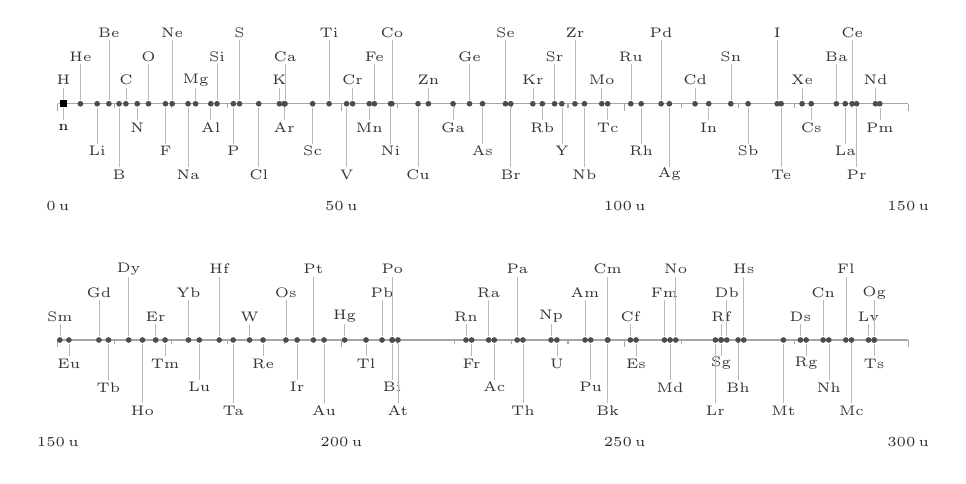
\begin{tikzpicture}[x=1mm, y=1mm, every node/.style={font=\tiny}]
\draw[gray!70] (0,0) -- (108,0);
\draw[gray!70] (0,-0.9) -- (0,0);
\node[anchor=north, text=gray!35!black] at (0,-11.2) {0\,u};
\draw[gray!70] (7.2,-0.5) -- (7.2,0);
\draw[gray!70] (14.4,-0.5) -- (14.4,0);
\draw[gray!70] (21.6,-0.5) -- (21.6,0);
\draw[gray!70] (28.8,-0.5) -- (28.8,0);
\draw[gray!70] (36,-0.9) -- (36,0);
\node[anchor=north, text=gray!35!black] at (36,-11.2) {50\,u};
\draw[gray!70] (43.2,-0.5) -- (43.2,0);
\draw[gray!70] (50.4,-0.5) -- (50.4,0);
\draw[gray!70] (57.6,-0.5) -- (57.6,0);
\draw[gray!70] (64.8,-0.5) -- (64.8,0);
\draw[gray!70] (72,-0.9) -- (72,0);
\node[anchor=north, text=gray!35!black] at (72,-11.2) {100\,u};
\draw[gray!70] (79.2,-0.5) -- (79.2,0);
\draw[gray!70] (86.4,-0.5) -- (86.4,0);
\draw[gray!70] (93.6,-0.5) -- (93.6,0);
\draw[gray!70] (100.8,-0.5) -- (100.8,0);
\draw[gray!70] (108,-0.9) -- (108,0);
\node[anchor=north, text=gray!35!black] at (108,-11.2) {150\,u};
\draw[gray!55, line width=0.2pt] (0.73,0.5) -- (0.73,2.05);
\node[fill=white, inner sep=0.15pt, text=black!80] at (0.73,3) {H};
\draw[gray!55, line width=0.2pt] (8.65,0.5) -- (8.65,2.05);
\node[fill=white, inner sep=0.15pt, text=black!80] at (8.65,3) {C};
\draw[gray!55, line width=0.2pt] (17.5,0.5) -- (17.5,2.05);
\node[fill=white, inner sep=0.15pt, text=black!80] at (17.5,3) {Mg};
\draw[gray!55, line width=0.2pt] (28.15,0.5) -- (28.15,2.05);
\node[fill=white, inner sep=0.15pt, text=black!80] at (28.15,3) {K};
\draw[gray!55, line width=0.2pt] (37.44,0.5) -- (37.44,2.05);
\node[fill=white, inner sep=0.15pt, text=black!80] at (37.44,3) {Cr};
\draw[gray!55, line width=0.2pt] (47.07,0.5) -- (47.07,2.05);
\node[fill=white, inner sep=0.15pt, text=black!80] at (47.07,3) {Zn};
\draw[gray!55, line width=0.2pt] (60.33,0.5) -- (60.33,2.05);
\node[fill=white, inner sep=0.15pt, text=black!80] at (60.33,3) {Kr};
\draw[gray!55, line width=0.2pt] (69.08,0.5) -- (69.08,2.05);
\node[fill=white, inner sep=0.15pt, text=black!80] at (69.08,3) {Mo};
\draw[gray!55, line width=0.2pt] (80.94,0.5) -- (80.94,2.05);
\node[fill=white, inner sep=0.15pt, text=black!80] at (80.94,3) {Cd};
\draw[gray!55, line width=0.2pt] (94.53,0.5) -- (94.53,2.05);
\node[fill=white, inner sep=0.15pt, text=black!80] at (94.53,3) {Xe};
\draw[gray!55, line width=0.2pt] (103.85,0.5) -- (103.85,2.05);
\node[fill=white, inner sep=0.15pt, text=black!80] at (103.85,3) {Nd};
\draw[gray!55, line width=0.2pt] (0.73,-0.5) -- (0.73,-2.05);
\node[fill=white, inner sep=0.15pt, text=black] at (0.73,-3) {n};
\draw[gray!55, line width=0.2pt] (10.09,-0.5) -- (10.09,-2.05);
\node[fill=white, inner sep=0.15pt, text=black!80] at (10.09,-3) {N};
\draw[gray!55, line width=0.2pt] (19.43,-0.5) -- (19.43,-2.05);
\node[fill=white, inner sep=0.15pt, text=black!80] at (19.43,-3) {Al};
\draw[gray!55, line width=0.2pt] (28.76,-0.5) -- (28.76,-2.05);
\node[fill=white, inner sep=0.15pt, text=black!80] at (28.76,-3) {Ar};
\draw[gray!55, line width=0.2pt] (39.56,-0.5) -- (39.56,-2.05);
\node[fill=white, inner sep=0.15pt, text=black!80] at (39.56,-3) {Mn};
\draw[gray!55, line width=0.2pt] (50.2,-0.5) -- (50.2,-2.05);
\node[fill=white, inner sep=0.15pt, text=black!80] at (50.2,-3) {Ga};
\draw[gray!55, line width=0.2pt] (61.54,-0.5) -- (61.54,-2.05);
\node[fill=white, inner sep=0.15pt, text=black!80] at (61.54,-3) {Rb};
\draw[gray!55, line width=0.2pt] (69.84,-0.5) -- (69.84,-2.05);
\node[fill=white, inner sep=0.15pt, text=black!80] at (69.84,-3) {Tc};
\draw[gray!55, line width=0.2pt] (82.67,-0.5) -- (82.67,-2.05);
\node[fill=white, inner sep=0.15pt, text=black!80] at (82.67,-3) {In};
\draw[gray!55, line width=0.2pt] (95.69,-0.5) -- (95.69,-2.05);
\node[fill=white, inner sep=0.15pt, text=black!80] at (95.69,-3) {Cs};
\draw[gray!55, line width=0.2pt] (104.4,-0.5) -- (104.4,-2.05);
\node[fill=white, inner sep=0.15pt, text=black!80] at (104.4,-3) {Pm};
\draw[gray!55, line width=0.2pt] (2.88,0.5) -- (2.88,5.05);
\node[fill=white, inner sep=0.15pt, text=black!80] at (2.88,6) {He};
\draw[gray!55, line width=0.2pt] (11.52,0.5) -- (11.52,5.05);
\node[fill=white, inner sep=0.15pt, text=black!80] at (11.52,6) {O};
\draw[gray!55, line width=0.2pt] (20.22,0.5) -- (20.22,5.05);
\node[fill=white, inner sep=0.15pt, text=black!80] at (20.22,6) {Si};
\draw[gray!55, line width=0.2pt] (28.86,0.5) -- (28.86,5.05);
\node[fill=white, inner sep=0.15pt, text=black!80] at (28.86,6) {Ca};
\draw[gray!55, line width=0.2pt] (40.21,0.5) -- (40.21,5.05);
\node[fill=white, inner sep=0.15pt, text=black!80] at (40.21,6) {Fe};
\draw[gray!55, line width=0.2pt] (52.29,0.5) -- (52.29,5.05);
\node[fill=white, inner sep=0.15pt, text=black!80] at (52.29,6) {Ge};
\draw[gray!55, line width=0.2pt] (63.09,0.5) -- (63.09,5.05);
\node[fill=white, inner sep=0.15pt, text=black!80] at (63.09,6) {Sr};
\draw[gray!55, line width=0.2pt] (72.77,0.5) -- (72.77,5.05);
\node[fill=white, inner sep=0.15pt, text=black!80] at (72.77,6) {Ru};
\draw[gray!55, line width=0.2pt] (85.47,0.5) -- (85.47,5.05);
\node[fill=white, inner sep=0.15pt, text=black!80] at (85.47,6) {Sn};
\draw[gray!55, line width=0.2pt] (98.88,0.5) -- (98.88,5.05);
\node[fill=white, inner sep=0.15pt, text=black!80] at (98.88,6) {Ba};
\draw[gray!55, line width=0.2pt] (5,-0.5) -- (5,-5.05);
\node[fill=white, inner sep=0.15pt, text=black!80] at (5,-6) {Li};
\draw[gray!55, line width=0.2pt] (13.68,-0.5) -- (13.68,-5.05);
\node[fill=white, inner sep=0.15pt, text=black!80] at (13.68,-6) {F};
\draw[gray!55, line width=0.2pt] (22.3,-0.5) -- (22.3,-5.05);
\node[fill=white, inner sep=0.15pt, text=black!80] at (22.3,-6) {P};
\draw[gray!55, line width=0.2pt] (32.37,-0.5) -- (32.37,-5.05);
\node[fill=white, inner sep=0.15pt, text=black!80] at (32.37,-6) {Sc};
\draw[gray!55, line width=0.2pt] (42.26,-0.5) -- (42.26,-5.05);
\node[fill=white, inner sep=0.15pt, text=black!80] at (42.26,-6) {Ni};
\draw[gray!55, line width=0.2pt] (53.94,-0.5) -- (53.94,-5.05);
\node[fill=white, inner sep=0.15pt, text=black!80] at (53.94,-6) {As};
\draw[gray!55, line width=0.2pt] (64.01,-0.5) -- (64.01,-5.05);
\node[fill=white, inner sep=0.15pt, text=black!80] at (64.01,-6) {Y};
\draw[gray!55, line width=0.2pt] (74.09,-0.5) -- (74.09,-5.05);
\node[fill=white, inner sep=0.15pt, text=black!80] at (74.09,-6) {Rh};
\draw[gray!55, line width=0.2pt] (87.67,-0.5) -- (87.67,-5.05);
\node[fill=white, inner sep=0.15pt, text=black!80] at (87.67,-6) {Sb};
\draw[gray!55, line width=0.2pt] (100.01,-0.5) -- (100.01,-5.05);
\node[fill=white, inner sep=0.15pt, text=black!80] at (100.01,-6) {La};
\draw[gray!55, line width=0.2pt] (6.49,0.5) -- (6.49,8.05);
\node[fill=white, inner sep=0.15pt, text=black!80] at (6.49,9) {Be};
\draw[gray!55, line width=0.2pt] (14.53,0.5) -- (14.53,8.05);
\node[fill=white, inner sep=0.15pt, text=black!80] at (14.53,9) {Ne};
\draw[gray!55, line width=0.2pt] (23.08,0.5) -- (23.08,8.05);
\node[fill=white, inner sep=0.15pt, text=black!80] at (23.08,9) {S};
\draw[gray!55, line width=0.2pt] (34.46,0.5) -- (34.46,8.05);
\node[fill=white, inner sep=0.15pt, text=black!80] at (34.46,9) {Ti};
\draw[gray!55, line width=0.2pt] (42.43,0.5) -- (42.43,8.05);
\node[fill=white, inner sep=0.15pt, text=black!80] at (42.43,9) {Co};
\draw[gray!55, line width=0.2pt] (56.86,0.5) -- (56.86,8.05);
\node[fill=white, inner sep=0.15pt, text=black!80] at (56.86,9) {Se};
\draw[gray!55, line width=0.2pt] (65.68,0.5) -- (65.68,8.05);
\node[fill=white, inner sep=0.15pt, text=black!80] at (65.68,9) {Zr};
\draw[gray!55, line width=0.2pt] (76.62,0.5) -- (76.62,8.05);
\node[fill=white, inner sep=0.15pt, text=black!80] at (76.62,9) {Pd};
\draw[gray!55, line width=0.2pt] (91.37,0.5) -- (91.37,8.05);
\node[fill=white, inner sep=0.15pt, text=black!80] at (91.37,9) {I};
\draw[gray!55, line width=0.2pt] (100.88,0.5) -- (100.88,8.05);
\node[fill=white, inner sep=0.15pt, text=black!80] at (100.88,9) {Ce};
\draw[gray!55, line width=0.2pt] (7.78,-0.5) -- (7.78,-8.05);
\node[fill=white, inner sep=0.15pt, text=black!80] at (7.78,-9) {B};
\draw[gray!55, line width=0.2pt] (16.55,-0.5) -- (16.55,-8.05);
\node[fill=white, inner sep=0.15pt, text=black!80] at (16.55,-9) {Na};
\draw[gray!55, line width=0.2pt] (25.52,-0.5) -- (25.52,-8.05);
\node[fill=white, inner sep=0.15pt, text=black!80] at (25.52,-9) {Cl};
\draw[gray!55, line width=0.2pt] (36.68,-0.5) -- (36.68,-8.05);
\node[fill=white, inner sep=0.15pt, text=black!80] at (36.68,-9) {V};
\draw[gray!55, line width=0.2pt] (45.75,-0.5) -- (45.75,-8.05);
\node[fill=white, inner sep=0.15pt, text=black!80] at (45.75,-9) {Cu};
\draw[gray!55, line width=0.2pt] (57.53,-0.5) -- (57.53,-8.05);
\node[fill=white, inner sep=0.15pt, text=black!80] at (57.53,-9) {Br};
\draw[gray!55, line width=0.2pt] (66.89,-0.5) -- (66.89,-8.05);
\node[fill=white, inner sep=0.15pt, text=black!80] at (66.89,-9) {Nb};
\draw[gray!55, line width=0.2pt] (77.67,-0.5) -- (77.67,-8.05);
\node[fill=white, inner sep=0.15pt, text=black!80] at (77.67,-9) {Ag};
\draw[gray!55, line width=0.2pt] (91.87,-0.5) -- (91.87,-8.05);
\node[fill=white, inner sep=0.15pt, text=black!80] at (91.87,-9) {Te};
\draw[gray!55, line width=0.2pt] (101.45,-0.5) -- (101.45,-8.05);
\node[fill=white, inner sep=0.15pt, text=black!80] at (101.45,-9) {Pr};
\fill[gray!60!black] (0.73,0) circle (0.36);
\fill (0.28,-0.45) rectangle (1.18,0.45);
\fill[gray!60!black] (2.88,0) circle (0.36);
\fill[gray!60!black] (5,0) circle (0.36);
\fill[gray!60!black] (6.49,0) circle (0.36);
\fill[gray!60!black] (7.78,0) circle (0.36);
\fill[gray!60!black] (8.65,0) circle (0.36);
\fill[gray!60!black] (10.09,0) circle (0.36);
\fill[gray!60!black] (11.52,0) circle (0.36);
\fill[gray!60!black] (13.68,0) circle (0.36);
\fill[gray!60!black] (14.53,0) circle (0.36);
\fill[gray!60!black] (16.55,0) circle (0.36);
\fill[gray!60!black] (17.5,0) circle (0.36);
\fill[gray!60!black] (19.43,0) circle (0.36);
\fill[gray!60!black] (20.22,0) circle (0.36);
\fill[gray!60!black] (22.3,0) circle (0.36);
\fill[gray!60!black] (23.08,0) circle (0.36);
\fill[gray!60!black] (25.52,0) circle (0.36);
\fill[gray!60!black] (28.15,0) circle (0.36);
\fill[gray!60!black] (28.76,0) circle (0.36);
\fill[gray!60!black] (28.86,0) circle (0.36);
\fill[gray!60!black] (32.37,0) circle (0.36);
\fill[gray!60!black] (34.46,0) circle (0.36);
\fill[gray!60!black] (36.68,0) circle (0.36);
\fill[gray!60!black] (37.44,0) circle (0.36);
\fill[gray!60!black] (39.56,0) circle (0.36);
\fill[gray!60!black] (40.21,0) circle (0.36);
\fill[gray!60!black] (42.26,0) circle (0.36);
\fill[gray!60!black] (42.43,0) circle (0.36);
\fill[gray!60!black] (45.75,0) circle (0.36);
\fill[gray!60!black] (47.07,0) circle (0.36);
\fill[gray!60!black] (50.2,0) circle (0.36);
\fill[gray!60!black] (52.29,0) circle (0.36);
\fill[gray!60!black] (53.94,0) circle (0.36);
\fill[gray!60!black] (56.86,0) circle (0.36);
\fill[gray!60!black] (57.53,0) circle (0.36);
\fill[gray!60!black] (60.33,0) circle (0.36);
\fill[gray!60!black] (61.54,0) circle (0.36);
\fill[gray!60!black] (63.09,0) circle (0.36);
\fill[gray!60!black] (64.01,0) circle (0.36);
\fill[gray!60!black] (65.68,0) circle (0.36);
\fill[gray!60!black] (66.89,0) circle (0.36);
\fill[gray!60!black] (69.08,0) circle (0.36);
\fill[gray!60!black] (69.84,0) circle (0.36);
\fill[gray!60!black] (72.77,0) circle (0.36);
\fill[gray!60!black] (74.09,0) circle (0.36);
\fill[gray!60!black] (76.62,0) circle (0.36);
\fill[gray!60!black] (77.67,0) circle (0.36);
\fill[gray!60!black] (80.94,0) circle (0.36);
\fill[gray!60!black] (82.67,0) circle (0.36);
\fill[gray!60!black] (85.47,0) circle (0.36);
\fill[gray!60!black] (87.67,0) circle (0.36);
\fill[gray!60!black] (91.37,0) circle (0.36);
\fill[gray!60!black] (91.87,0) circle (0.36);
\fill[gray!60!black] (94.53,0) circle (0.36);
\fill[gray!60!black] (95.69,0) circle (0.36);
\fill[gray!60!black] (98.88,0) circle (0.36);
\fill[gray!60!black] (100.01,0) circle (0.36);
\fill[gray!60!black] (100.88,0) circle (0.36);
\fill[gray!60!black] (101.45,0) circle (0.36);
\fill[gray!60!black] (103.85,0) circle (0.36);
\fill[gray!60!black] (104.4,0) circle (0.36);
\draw[gray!70] (0,-30) -- (108,-30);
\draw[gray!70] (0,-30.9) -- (0,-30);
\node[anchor=north, text=gray!35!black] at (0,-41.2) {150\,u};
\draw[gray!70] (7.2,-30.5) -- (7.2,-30);
\draw[gray!70] (14.4,-30.5) -- (14.4,-30);
\draw[gray!70] (21.6,-30.5) -- (21.6,-30);
\draw[gray!70] (28.8,-30.5) -- (28.8,-30);
\draw[gray!70] (36,-30.9) -- (36,-30);
\node[anchor=north, text=gray!35!black] at (36,-41.2) {200\,u};
\draw[gray!70] (43.2,-30.5) -- (43.2,-30);
\draw[gray!70] (50.4,-30.5) -- (50.4,-30);
\draw[gray!70] (57.6,-30.5) -- (57.6,-30);
\draw[gray!70] (64.8,-30.5) -- (64.8,-30);
\draw[gray!70] (72,-30.9) -- (72,-30);
\node[anchor=north, text=gray!35!black] at (72,-41.2) {250\,u};
\draw[gray!70] (79.2,-30.5) -- (79.2,-30);
\draw[gray!70] (86.4,-30.5) -- (86.4,-30);
\draw[gray!70] (93.6,-30.5) -- (93.6,-30);
\draw[gray!70] (100.8,-30.5) -- (100.8,-30);
\draw[gray!70] (108,-30.9) -- (108,-30);
\node[anchor=north, text=gray!35!black] at (108,-41.2) {300\,u};
\draw[gray!55, line width=0.2pt] (0.26,-29.5) -- (0.26,-27.95);
\node[fill=white, inner sep=0.15pt, text=black!80] at (0.26,-27) {Sm};
\draw[gray!55, line width=0.2pt] (12.43,-29.5) -- (12.43,-27.95);
\node[fill=white, inner sep=0.15pt, text=black!80] at (12.43,-27) {Er};
\draw[gray!55, line width=0.2pt] (24.36,-29.5) -- (24.36,-27.95);
\node[fill=white, inner sep=0.15pt, text=black!80] at (24.36,-27) {W};
\draw[gray!55, line width=0.2pt] (36.43,-29.5) -- (36.43,-27.95);
\node[fill=white, inner sep=0.15pt, text=black!80] at (36.43,-27) {Hg};
\draw[gray!55, line width=0.2pt] (51.84,-29.5) -- (51.84,-27.95);
\node[fill=white, inner sep=0.15pt, text=black!80] at (51.84,-27) {Rn};
\draw[gray!55, line width=0.2pt] (62.64,-29.5) -- (62.64,-27.95);
\node[fill=white, inner sep=0.15pt, text=black!80] at (62.64,-27) {Np};
\draw[gray!55, line width=0.2pt] (72.72,-29.5) -- (72.72,-27.95);
\node[fill=white, inner sep=0.15pt, text=black!80] at (72.72,-27) {Cf};
\draw[gray!55, line width=0.2pt] (84.24,-29.5) -- (84.24,-27.95);
\node[fill=white, inner sep=0.15pt, text=black!80] at (84.24,-27) {Rf};
\draw[gray!55, line width=0.2pt] (94.32,-29.5) -- (94.32,-27.95);
\node[fill=white, inner sep=0.15pt, text=black!80] at (94.32,-27) {Ds};
\draw[gray!55, line width=0.2pt] (102.96,-29.5) -- (102.96,-27.95);
\node[fill=white, inner sep=0.15pt, text=black!80] at (102.96,-27) {Lv};
\draw[gray!55, line width=0.2pt] (1.41,-30.5) -- (1.41,-32.05);
\node[fill=white, inner sep=0.15pt, text=black!80] at (1.41,-33) {Eu};
\draw[gray!55, line width=0.2pt] (13.63,-30.5) -- (13.63,-32.05);
\node[fill=white, inner sep=0.15pt, text=black!80] at (13.63,-33) {Tm};
\draw[gray!55, line width=0.2pt] (26.07,-30.5) -- (26.07,-32.05);
\node[fill=white, inner sep=0.15pt, text=black!80] at (26.07,-33) {Re};
\draw[gray!55, line width=0.2pt] (39.15,-30.5) -- (39.15,-32.05);
\node[fill=white, inner sep=0.15pt, text=black!80] at (39.15,-33) {Tl};
\draw[gray!55, line width=0.2pt] (52.56,-30.5) -- (52.56,-32.05);
\node[fill=white, inner sep=0.15pt, text=black!80] at (52.56,-33) {Fr};
\draw[gray!55, line width=0.2pt] (63.38,-30.5) -- (63.38,-32.05);
\node[fill=white, inner sep=0.15pt, text=black!80] at (63.38,-33) {U};
\draw[gray!55, line width=0.2pt] (73.44,-30.5) -- (73.44,-32.05);
\node[fill=white, inner sep=0.15pt, text=black!80] at (73.44,-33) {Es};
\draw[gray!55, line width=0.2pt] (84.24,-30.5) -- (84.24,-32.05);
\node[fill=white, inner sep=0.15pt, text=black!80] at (84.24,-33) {Sg};
\draw[gray!55, line width=0.2pt] (95.04,-30.5) -- (95.04,-32.05);
\node[fill=white, inner sep=0.15pt, text=black!80] at (95.04,-33) {Rg};
\draw[gray!55, line width=0.2pt] (103.68,-30.5) -- (103.68,-32.05);
\node[fill=white, inner sep=0.15pt, text=black!80] at (103.68,-33) {Ts};
\draw[gray!55, line width=0.2pt] (5.22,-29.5) -- (5.22,-24.95);
\node[fill=white, inner sep=0.15pt, text=black!80] at (5.22,-24) {Gd};
\draw[gray!55, line width=0.2pt] (16.59,-29.5) -- (16.59,-24.95);
\node[fill=white, inner sep=0.15pt, text=black!80] at (16.59,-24) {Yb};
\draw[gray!55, line width=0.2pt] (28.97,-29.5) -- (28.97,-24.95);
\node[fill=white, inner sep=0.15pt, text=black!80] at (28.97,-24) {Os};
\draw[gray!55, line width=0.2pt] (41.18,-29.5) -- (41.18,-24.95);
\node[fill=white, inner sep=0.15pt, text=black!80] at (41.18,-24) {Pb};
\draw[gray!55, line width=0.2pt] (54.72,-29.5) -- (54.72,-24.95);
\node[fill=white, inner sep=0.15pt, text=black!80] at (54.72,-24) {Ra};
\draw[gray!55, line width=0.2pt] (66.96,-29.5) -- (66.96,-24.95);
\node[fill=white, inner sep=0.15pt, text=black!80] at (66.96,-24) {Am};
\draw[gray!55, line width=0.2pt] (77.04,-29.5) -- (77.04,-24.95);
\node[fill=white, inner sep=0.15pt, text=black!80] at (77.04,-24) {Fm};
\draw[gray!55, line width=0.2pt] (84.96,-29.5) -- (84.96,-24.95);
\node[fill=white, inner sep=0.15pt, text=black!80] at (84.96,-24) {Db};
\draw[gray!55, line width=0.2pt] (97.2,-29.5) -- (97.2,-24.95);
\node[fill=white, inner sep=0.15pt, text=black!80] at (97.2,-24) {Cn};
\draw[gray!55, line width=0.2pt] (103.68,-29.5) -- (103.68,-24.95);
\node[fill=white, inner sep=0.15pt, text=black!80] at (103.68,-24) {Og};
\draw[gray!55, line width=0.2pt] (6.43,-30.5) -- (6.43,-35.05);
\node[fill=white, inner sep=0.15pt, text=black!80] at (6.43,-36) {Tb};
\draw[gray!55, line width=0.2pt] (17.98,-30.5) -- (17.98,-35.05);
\node[fill=white, inner sep=0.15pt, text=black!80] at (17.98,-36) {Lu};
\draw[gray!55, line width=0.2pt] (30.4,-30.5) -- (30.4,-35.05);
\node[fill=white, inner sep=0.15pt, text=black!80] at (30.4,-36) {Ir};
\draw[gray!55, line width=0.2pt] (42.47,-30.5) -- (42.47,-35.05);
\node[fill=white, inner sep=0.15pt, text=black!80] at (42.47,-36) {Bi};
\draw[gray!55, line width=0.2pt] (55.44,-30.5) -- (55.44,-35.05);
\node[fill=white, inner sep=0.15pt, text=black!80] at (55.44,-36) {Ac};
\draw[gray!55, line width=0.2pt] (67.68,-30.5) -- (67.68,-35.05);
\node[fill=white, inner sep=0.15pt, text=black!80] at (67.68,-36) {Pu};
\draw[gray!55, line width=0.2pt] (77.76,-30.5) -- (77.76,-35.05);
\node[fill=white, inner sep=0.15pt, text=black!80] at (77.76,-36) {Md};
\draw[gray!55, line width=0.2pt] (86.4,-30.5) -- (86.4,-35.05);
\node[fill=white, inner sep=0.15pt, text=black!80] at (86.4,-36) {Bh};
\draw[gray!55, line width=0.2pt] (97.92,-30.5) -- (97.92,-35.05);
\node[fill=white, inner sep=0.15pt, text=black!80] at (97.92,-36) {Nh};
\draw[gray!55, line width=0.2pt] (9,-29.5) -- (9,-21.95);
\node[fill=white, inner sep=0.15pt, text=black!80] at (9,-21) {Dy};
\draw[gray!55, line width=0.2pt] (20.51,-29.5) -- (20.51,-21.95);
\node[fill=white, inner sep=0.15pt, text=black!80] at (20.51,-21) {Hf};
\draw[gray!55, line width=0.2pt] (32.46,-29.5) -- (32.46,-21.95);
\node[fill=white, inner sep=0.15pt, text=black!80] at (32.46,-21) {Pt};
\draw[gray!55, line width=0.2pt] (42.48,-29.5) -- (42.48,-21.95);
\node[fill=white, inner sep=0.15pt, text=black!80] at (42.48,-21) {Po};
\draw[gray!55, line width=0.2pt] (58.35,-29.5) -- (58.35,-21.95);
\node[fill=white, inner sep=0.15pt, text=black!80] at (58.35,-21) {Pa};
\draw[gray!55, line width=0.2pt] (69.84,-29.5) -- (69.84,-21.95);
\node[fill=white, inner sep=0.15pt, text=black!80] at (69.84,-21) {Cm};
\draw[gray!55, line width=0.2pt] (78.48,-29.5) -- (78.48,-21.95);
\node[fill=white, inner sep=0.15pt, text=black!80] at (78.48,-21) {No};
\draw[gray!55, line width=0.2pt] (87.12,-29.5) -- (87.12,-21.95);
\node[fill=white, inner sep=0.15pt, text=black!80] at (87.12,-21) {Hs};
\draw[gray!55, line width=0.2pt] (100.08,-29.5) -- (100.08,-21.95);
\node[fill=white, inner sep=0.15pt, text=black!80] at (100.08,-21) {Fl};
\draw[gray!55, line width=0.2pt] (10.75,-30.5) -- (10.75,-38.05);
\node[fill=white, inner sep=0.15pt, text=black!80] at (10.75,-39) {Ho};
\draw[gray!55, line width=0.2pt] (22.28,-30.5) -- (22.28,-38.05);
\node[fill=white, inner sep=0.15pt, text=black!80] at (22.28,-39) {Ta};
\draw[gray!55, line width=0.2pt] (33.82,-30.5) -- (33.82,-38.05);
\node[fill=white, inner sep=0.15pt, text=black!80] at (33.82,-39) {Au};
\draw[gray!55, line width=0.2pt] (43.2,-30.5) -- (43.2,-38.05);
\node[fill=white, inner sep=0.15pt, text=black!80] at (43.2,-39) {At};
\draw[gray!55, line width=0.2pt] (59.07,-30.5) -- (59.07,-38.05);
\node[fill=white, inner sep=0.15pt, text=black!80] at (59.07,-39) {Th};
\draw[gray!55, line width=0.2pt] (69.84,-30.5) -- (69.84,-38.05);
\node[fill=white, inner sep=0.15pt, text=black!80] at (69.84,-39) {Bk};
\draw[gray!55, line width=0.2pt] (83.52,-30.5) -- (83.52,-38.05);
\node[fill=white, inner sep=0.15pt, text=black!80] at (83.52,-39) {Lr};
\draw[gray!55, line width=0.2pt] (92.16,-30.5) -- (92.16,-38.05);
\node[fill=white, inner sep=0.15pt, text=black!80] at (92.16,-39) {Mt};
\draw[gray!55, line width=0.2pt] (100.8,-30.5) -- (100.8,-38.05);
\node[fill=white, inner sep=0.15pt, text=black!80] at (100.8,-39) {Mc};
\fill[gray!60!black] (0.26,-30) circle (0.36);
\fill[gray!60!black] (1.41,-30) circle (0.36);
\fill[gray!60!black] (5.22,-30) circle (0.36);
\fill[gray!60!black] (6.43,-30) circle (0.36);
\fill[gray!60!black] (9,-30) circle (0.36);
\fill[gray!60!black] (10.75,-30) circle (0.36);
\fill[gray!60!black] (12.43,-30) circle (0.36);
\fill[gray!60!black] (13.63,-30) circle (0.36);
\fill[gray!60!black] (16.59,-30) circle (0.36);
\fill[gray!60!black] (17.98,-30) circle (0.36);
\fill[gray!60!black] (20.51,-30) circle (0.36);
\fill[gray!60!black] (22.28,-30) circle (0.36);
\fill[gray!60!black] (24.36,-30) circle (0.36);
\fill[gray!60!black] (26.07,-30) circle (0.36);
\fill[gray!60!black] (28.97,-30) circle (0.36);
\fill[gray!60!black] (30.4,-30) circle (0.36);
\fill[gray!60!black] (32.46,-30) circle (0.36);
\fill[gray!60!black] (33.82,-30) circle (0.36);
\fill[gray!60!black] (36.43,-30) circle (0.36);
\fill[gray!60!black] (39.15,-30) circle (0.36);
\fill[gray!60!black] (41.18,-30) circle (0.36);
\fill[gray!60!black] (42.47,-30) circle (0.36);
\fill[gray!60!black] (42.48,-30) circle (0.36);
\fill[gray!60!black] (43.2,-30) circle (0.36);
\fill[gray!60!black] (51.84,-30) circle (0.36);
\fill[gray!60!black] (52.56,-30) circle (0.36);
\fill[gray!60!black] (54.72,-30) circle (0.36);
\fill[gray!60!black] (55.44,-30) circle (0.36);
\fill[gray!60!black] (58.35,-30) circle (0.36);
\fill[gray!60!black] (59.07,-30) circle (0.36);
\fill[gray!60!black] (62.64,-30) circle (0.36);
\fill[gray!60!black] (63.38,-30) circle (0.36);
\fill[gray!60!black] (66.96,-30) circle (0.36);
\fill[gray!60!black] (67.68,-30) circle (0.36);
\fill[gray!60!black] (69.84,-30) circle (0.36);
\fill[gray!60!black] (69.84,-30) circle (0.36);
\fill[gray!60!black] (72.72,-30) circle (0.36);
\fill[gray!60!black] (73.44,-30) circle (0.36);
\fill[gray!60!black] (77.04,-30) circle (0.36);
\fill[gray!60!black] (77.76,-30) circle (0.36);
\fill[gray!60!black] (78.48,-30) circle (0.36);
\fill[gray!60!black] (83.52,-30) circle (0.36);
\fill[gray!60!black] (84.24,-30) circle (0.36);
\fill[gray!60!black] (84.24,-30) circle (0.36);
\fill[gray!60!black] (84.96,-30) circle (0.36);
\fill[gray!60!black] (86.4,-30) circle (0.36);
\fill[gray!60!black] (87.12,-30) circle (0.36);
\fill[gray!60!black] (92.16,-30) circle (0.36);
\fill[gray!60!black] (94.32,-30) circle (0.36);
\fill[gray!60!black] (95.04,-30) circle (0.36);
\fill[gray!60!black] (97.2,-30) circle (0.36);
\fill[gray!60!black] (97.92,-30) circle (0.36);
\fill[gray!60!black] (100.08,-30) circle (0.36);
\fill[gray!60!black] (100.8,-30) circle (0.36);
\fill[gray!60!black] (102.96,-30) circle (0.36);
\fill[gray!60!black] (103.68,-30) circle (0.36);
\fill[gray!60!black] (103.68,-30) circle (0.36);
\end{tikzpicture}
}
\caption[The atoms on the mass axis]{The mass axis of \Cref{fig:standard-model}, unrolled: the 118 atoms and the neutron (square) at $r = m$, in daltons, in two lines from $0$ to $150$ u and from $150$ to $300$ u.}
\label{fig:sm-ruler}
\end{figure}

\subsection{The Standard Model in Six Lines}\label{subsec:sm-summary}

\Cref{tab:sm-summary} gathers the road of this chapter. Each line uses only what the lines above it established.

\begin{table}[tb]
\myfloatalign
\small
\begin{tabularx}{\textwidth}{@{}l >{\raggedright\arraybackslash}X >{\raggedright\arraybackslash}X@{}}
\toprule
\tableheadline{step} & \tableheadline{what is built} & \tableheadline{the formula} \\
\midrule
1 & one body, one triangle & $\alpha + \phi = \pb$; corner $100.14^\circ$; $q\Gp = z\,m_S$ \\
2 & all triangles of one size & $m^2 + (q\Gp)^2 + 0.35210\,m\,q\Gp = r^2$ \\
3 & the frame & rings of equal $r$, rays of equal $\alpha$ \\
4 & where matter falls & $r = m$ or $r = |z|\,m_S$; $\delta \approx 5.0374 \times 10^{-17}{}^\circ \times m/|z|$ \\
5 & the cards & $m_{\text{ion}} = A - z\,m_e$; $m_{\text{nucleus}} = A - Z\,m_e + B_e/c^2$ \\
6 & the standard model & 306 bodies on three directions of one frame \\
\bottomrule
\end{tabularx}
\caption[The standard model in six lines]{The Cosmic Mass Standard Model in six lines, all at the angle $79.86^\circ$ of the Composer axis.}
\label{tab:sm-summary}
\end{table}

\subsection{What the Model Is, and What It Is Not}\label{subsec:sm-is-not}

The Cosmic Mass Standard Model is a frame and a catalogue. It takes two numbers that physics has measured for every body, the mass and the charge, and writes them as one magnitude and two angles in a single geometry, built from one fixed angle. Everything in it can be checked with a spreadsheet, and the workbook that comes with this book does so for all 306 bodies.

It is not a new law of nature. It predicts no new particle, and it moves no measured mass or charge. What it adds is a language: a single picture in which neutral matter, ions and nuclei stand side by side; a reading of the charge-to-mass ratio as an angle, exactly the quantity that Thomson's tube and Aston's spectrograph measured; and a family of ellipses whose shape is fixed by the angle of the Composer axis alone.

One question remains open, and Chapter~\ref{ch:alignment} names it as the work of Volume~2: the physical meaning of the Composer coordinate of a product, which holds the Coupling term and a share of the term of two charges, by far the larger for charged particles (\Cref{subsec:law-read}), but is not read as a force (Definition~\ref{def:reading}). The frame itself rests on the angle $79.86^\circ$ of the Composer axis (Remark~\ref{rem:sm-fixed-angle}): its corner angle of $100.14^\circ$, its coefficient $0.35210$ and its lean of $5.0374 \times 10^{-17}$ degree per dalton all come from that angle. Until the Composer coordinate is tied to a measurement, the model is a more expressive way to see the bodies we know, which is exactly what it sets out to be.

\begin{plainwords}
Start with one angle, $79.86^\circ$, the angle at which like charges push apart (Chapter~\ref{ch:interaction}). Draw every body as a triangle whose corner always has the same angle. All the triangles of one size line up on an ellipse; the ellipses of all sizes, with the rays of equal angle, make graph paper. On that paper, every neutral body sits on one line, every positive body near a second line and every negative body near a third, each tipped by its mass per charge. That picture, with all 306 bodies in it, is the Cosmic Mass Standard Model.
\end{plainwords}
